% -*- Mode:TeX -*-

%% The documentclass options along with the pagestyle can be used to generate
%% a technical report, a draft copy, or a regular thesis.  You may need to
%% re-specify the pagestyle after you \include  cover.tex.  For more
%% information, see the first few lines of mitthesis.cls. 

%\documentclass[12pt,vi,twoside]{mitthesis}
%%
%%  If you want your thesis copyright to you instead of MIT, use the
%%  ``vi'' option, as above.
%%
%\documentclass[12pt,twoside,leftblank]{mitthesis}
%%
%% If you want blank pages before new chapters to be labelled ``This
%% Page Intentionally Left Blank'', use the ``leftblank'' option, as
%% above. 

\documentclass[12pt,twoside]{mitthesis}
\usepackage[left=1in, right=1in, top=1in, bottom=1in]{geometry} 
\usepackage{lgrind}
\usepackage{graphicx}
\usepackage{amsmath}
\usepackage{amssymb}
\usepackage{subfigure}
\usepackage[small, width = .9\textwidth, center]{caption}
\usepackage{tikz}
\usepackage{natbib}
\usepackage{bm}
\usepackage{epstopdf}
\usepackage{listings}
\usepackage{color}
\usepackage[hyphens]{url}
\usepackage{multirow}
\PassOptionsToPackage{hyphens}{url}\usepackage[hidelinks]{hyperref}
\usepackage{quotchap}
\usepackage{bbm}
\usepackage{textcomp}
\pagestyle{plain}

\definecolor{dkgreen}{rgb}{0,0.6,0}
\definecolor{gray}{rgb}{0.5,0.5,0.5}
\definecolor{mauve}{rgb}{0.58,0,0.82}

\lstdefinelanguage{XML} {
  morestring=[s]{>}{<},
  identifierstyle=\color{blue},
}

\lstset{frame=tb,
  language=Java,
  aboveskip=3mm,
  belowskip=3mm,
  showstringspaces=false,
  columns=flexible,
  basicstyle={\small\ttfamily},
  numbers=none,
  numberstyle=\tiny\color{gray},
  keywordstyle=\color{blue},
  commentstyle=\color{dkgreen},
  stringstyle=\color{mauve},
  breaklines=true,
  breakatwhitespace=true,
  tabsize=2,
  lineskip={-0.05pt}
}

%% This bit allows you to either specify only the files which you wish to
%% process, or `all' to process all files which you \include.
%% Krishna Sethuraman (1990).

%\typein [\files]{Enter file names to process, (chap1,chap2 ...), or `all' toprocess all files:}
%\def\all{all}
%\ifx\files\all \typeout{Including all files.} \else \typeout{Including only \files.} \includeonly{\files} \fi
\newcommand{\superscript}[1]{\ensuremath{^{\textrm{#1}}}}
\newcommand{\subscript}[1]{\ensuremath{_{\textrm{#1}}}}
\newcommand{\eqdef}{\overset{\mathrm{def}}{=\joinrel=}}
\newcommand*{\thead}[1]{\multicolumn{1}{|c|}{\bfseries #1}}

\makeatletter
\providecommand*{\diff}%
{\@ifnextchar^{\DIfF}{\DIfF^{}}}
\def\DIfF^#1{%
\mathop{\mathrm{\mathstrut d}}%
\nolimits^{#1}\gobblespace}
\def\gobblespace{%
\futurelet\diffarg\opspace}
\def\opspace{%
\let\DiffSpace\!%
\ifx\diffarg(%
\let\DiffSpace\relax
\else
\ifx\diffarg[%
\let\DiffSpace\relax
\else
\ifx\diffarg\{%
\let\DiffSpace\relax
\fi\fi\fi\DiffSpace}

\begin{document}

\include{cover}
\pagestyle{plain}
\tableofcontents
\listoffigures
\listoftables
\begin{savequote}
Gesture is a critical link running through the evolution of perception,
conceptualization, and language.
\qauthor{David Armstrong, William Stokoe, and Sherman Wilcox, \textit{Gesture
and the nature of language}}
\end{savequote}
\chapter{Introduction}
% (Start with a motivating scenario: either Powerpoint presentation or USAR
% application.)
% \begin{quotation}
% \textit{Imagine an earthquake has hit a populous area and many major roads are
% impassable. Buildings are severely damaged or collapsed, and fire has broken out
% in many places. At the crisis management center, response professionals are
% working together to coordinate the earthquake relief effort. You are the
% incident commander charged with coordinating the search
% and rescue teams working in the field. There is a large tabletop display in
% front of you, showing the map of the site. Information coming from the field is
% updated on the display in real-time.}
% 
% \textit{A report about a big explosion at a chemical plant comes in and you move
% the map around, zoom in and rotate it to get a good view of the plant. On the
% map, you see there is a group of unmanned vehicles nearby. After selecting them
% on the map with your hand, you speak to the interface ``Go nearer to the
% explosion site to gather more information,'' while tracing the route the
% vehicles should take to avoid obstacles. Then you instruct rescue team No. 3 to evacuate the residents
% in the surrounding buildings by going under a bridge because the surface of the
% bridge is blocked. You gesture with one hand as the bridge and the other
% hand moving under it to emphasize this.}
% \end{quotation}
% 
% The scenario above is an example in the Urban Search and Rescue (USAR) domain.
% It shows an application of a multi-modal interface to a real-world problem. Gestures play an important part in this scenario,
% providing key information about location, method and timing of movements,
% and about spatial relationship among the objects being described.
\begin{quotation}
Imagine how nice it would be, the next time you make a presentation, if you did not need to stand close to your laptop or use a remote control with its limited functionality. What if you could present your work as naturally as having a conversation with your audience. You swipe your hand left and right to change slides. When you point to the slide with your hand, the display shows a pointer cursor following wherever you point. When you are showing a video, you use a palm forward hand pose (�stop� gesture) to pause the movie, then move left and right to fast forward or rewind the video. You can also say �faster� or �slower� to change the video speed. When you need to jump to a particular slide, you make a circle gesture to show all the slides, and say "show this slide'' while pointing at that slide. You can also make a dismiss gesture to pause the slide show (making the screen black) to take the distracting slides off the screen and get full attention from the audience during presentation.

\end{quotation}

The above scenario shows an application of a multimodal interface to a
real-world problem, with different types of gestures playing an important part
in the scenario.
 
Recent trends in user interfaces have brought on a new wave of interaction
techniques that depart from the traditional mouse and keyboard that have been 
used for decades. These include multi-touch interfaces such as the 
iPhone, the iPad and the Microsoft 
Surface\textsuperscript{\textregistered} as well as camera-based systems such as
the Microsoft Kinect and the Leap Motion sensor. Most
of these devices gained instant popularity among consumers, and the common trait
among them is that they make interacting with computation more natural and 
effortless. All these devices allow users to use their hands and/or body 
gestures to directly manipulate virtual objects. It feels more natural this 
way because this is how we interact with our environment in everyday life.
 
There is also a trend in wearable human-computer interfaces recently pioneered
by products such as Google Glass, Samsung's Galaxy Gear smartwatches and Pebble
smartwatches. These products have potential for gesture input as well. Google
Glass has a camera which can be used to recognize hand motion and hand shapes.
The accelerometers in the smartwatches can also be used to measure hand motion,
just like the Nintendo Wii controller.

There are big potential and demand for natural interaction, and gesture is
an important part of it. We start to see more and more gestural interfaces,
however, many of them still mainly make the hands function as a mouse with a
limited number of other gestures. Our goal is to break out from the old
paradigm of ``point, click, drag'' interaction we used to have with mice. 
Our hands are much more versatile, and hence, I believe that to design a gesture
recognition system for natural human computer interaction (HCI), we need to
start from the user interaction perspective: what are the different types of
gestures people use; when should the system respond; how should the model be
defined and trained; and how to combine gesture and speech for natural
interaction. These are the questions I addressed in this thesis. Based on my
findings, I developed a real-time continuous gesture recognition and
interaction system that handles different types of gestures seamlessly, and
responds to gestures appropriately.

\section{Background}
To design a natural gestural interface, it is important to understand the
nature of human gestures. This section gives some background information in
gesture production and taxonomy, and introduces several important concepts and
terms that are central to the final system design.
 
\subsection{Definition of Gestures}
Webster's Dictionary defines gestures as ``\ldots a movement usually of the body or limbs
that expresses or emphasizes an idea, sentiment, or attitude.'' This definition
is particularly related to the communicational aspect of the human hand and body
movements. However, in HCI, the notion
of gestures is somewhat different. In their review of the visual interpretation
of hand gestures for HCI, Pavlovic et al. \cite{Pavlovic97} states that in a computer
controlled environment one wants to use the human hand to perform tasks that
mimic both the natural use of the hand as a manipulator, and its use in
human-machine communication. They include both manipulative and communicative
gestures in their gesture taxonomy. This is also the definition I use in
the thesis.

Pavlovic et al. \cite{Pavlovic97} also gives a model (Figure. 
\ref{fig:gesture_production}) for the production and perception of gestures 
based on the model used in the field of spoken language recognition. According 
to their model, gestures originate as a gesturer's mental concept, possibly in 
conjunction with speech. They are expressed through the motion of arms and 
hands. Also, observers perceive gestures as streams of visual images which they
interpret using their knowledge about those gestures. In HCI, the 
observer is the computer and the knowledge it possesses is the training data we 
give it.

\begin{figure}[tbh]
  \centering
  \includegraphics[width=0.7\textwidth]{figures/gesture_production.png} 
  \caption{Production and perception of gestures. Hand gestures originate as a
  mental concept, are expressed through arm and hand motion, and are perceived
  as visual images \cite{Pavlovic97}.}
  \label{fig:gesture_production}
\end{figure}

Kendon~\cite{kendon86} distinguishes \textit{autonomous gestures} from
\textit{gesticulation}, gestures that occur in association with speech. We focus
on autonomous gestures.

\subsection{Gestural Taxonomy}\label{sec:taxonomy}
The mental concept of a gesture represents the semantic meaning or the
actual intention of the gesturer. In this dimension, hand movements can be
divided into different general categories. Each category has its own characteristics and requires different responses from the computer interface. Having a systematic gesture taxonomy can inform
us about the design of the interactive system. The taxonomy will also be the
basis of our hierarchical approach to gesture interpretation. Our gesture
taxonomy (see Figure \ref{fig:taxonomy}) is based on the one developed by Pavlovic et al.
\cite{Pavlovic97} with some changes to make the terminology clearer. This is
also similar to the \textit{nature} dimension in the taxonomy proposed by
Wobbrock et al. \cite{wobbrock09}

\begin{figure}[h]
  \centering
  \includegraphics[width=0.5\textwidth]{figures/taxonomy.png} 
  \caption{Gesture taxonomy}
  \label{fig:taxonomy}
\end{figure}

First, gestures, as \textit{intentional} movements, should be distinguished from
\textit{unintentional} hand movements (like beats). By \textit{unintentional}
movements, we mean movements that are not intended to convey information. In
contrast, gestures are meaningful hand movements that people make to convey some
information. The distinction is important for a natural interface because there
should not be any restriction on how people should place or move their hands
when they are not doing any meaningful gestures. 

Gestures are then further divided into manipulative and communicative
categories. Manipulative gestures are used to act on objects (e.g.
moving an virtual object around, click a button, the property of the virtual
object change directly according to certain parameters of the hand(s)), while
communicative gestures have an inherent purpose for communication \cite{Pavlovic97}. 
the meaning of the gesture when the user finishes performing the gesture. This part is
accomplished by gesture recognition. So manipulative gestures and communicative
gestures fall into the \textit{continuous} category and the
\textit{discrete} category respectively in the \textit{flow} dimension of the
taxonomy proposed by Wobbrock \cite{wobbrock09} et al. based on their
user study.

People perform communicative gestures via acts or symbols. Gesture via acts are
those directly related to the interpretation of the movement itself. Such
movements are classified as either mimetic (which imitate some actions) or
deictic (pointing acts that convey spatial information). Gestures via symbols
are those that have a linguistic role, and are often represented by different static hand postures. An example is forming the
O.K. pose for ``accept''. 

\subsection{Gesture Form and Flow}
Wobbrock et al. \cite{wobbrock09} classified gestures into four dimensions:
\textit{form}, \textit{nature}, \textit{binding}, and \textit{flow}. These
dimensions are orthogonal. We looked into the \textit{form} and the
\textit{flow} dimensions. The \textit{form} dimension is particularly important
for building the gesture recognition model because different forms constitute
different features we need to consider. The \textit{binding} and \textit{flow}
dimensions are relevant for the application layer because they are related to
how the user interface should respond to gesture events.

However, we take a different definition on gesture with dynamic paths. In their
paper, they refer dynamic paths as any gestures that involve change of hand
locations. However, we consider gestures with dynamic paths as gestures with a
well-defined paths. For example, a ``Swipe Left'' gesture has a dynamic path,
where as a ``Pointing'' gesture with moving hand to indicate different locations
is not considered as gestures with dynamic path because the path is not
well-defined (the user is likely to move anywhere as he/she wants). The reason
for this distinction is that gestures with well-defined paths are suitable to be
model by sequential data models such as HMMs.

The physical arm and hand movements that express
the mental concept of the gesture can be categorized into different \textit{forms} \cite{wobbrock09} as shown in Table \ref{tab:form}. Both manipulative and communicative gestures can
have all of these forms. This means that the features we want to use for
gestural analysis should be based on both the hand pose and the locus of the
hand movement.

\begin{table}[h]
  \centering
  \begin{tabular}{| l | l |}
  	\hline
  	\textbf{Form} 		  & \textbf{Description} \\ \hline 
  	Static pose  		  & Hand pose is held in one location. \\ \hline
  	Dynamic pose 		  & Hand pose changes while location does not. \\ \hline
  	Static pose and path  & Hand pose is held as hand moves. \\ \hline
  	Dynamic pose and path & Hand pose changes as hand moves. \\ \hline
  \end{tabular}
  \caption{Different gesture forms.}
  \label{tab:form}
\end{table}

To respond properly, the system must differentiate discrete and continuous
flow gestures. If a gesture's flow
is discrete, the whole sequence needs to be delimited, recognized, and responded
as a single event. For example, a \textit{wave} gesture that can mean ``no'' or getting the attention of the 
system should be responded at the end of the gesture. On the other hand, if the 
flow is continuous, ongoing system response is required. Consider the \textit{pan} and the \textit{resize} gestures, 
as the user moves his/her hand(s), the system has to respond in each frame such that
certain parameter(s) of the virtual object(s) that the user is controlling are tied to
certain parameter(s) of the user's hand(s).

One major distinction between discrete and continuous flow gestures is that,
in a pre-defined gesture set, discrete flow gestures usually have specific hand
poses and movement paths, where continuous flow gestures usually do not have
specific movement paths, but can have specific hand poses.
For example, when panning, the user's hand may move in any
direction. As a result, 
 we cannot train the system with examples of  the
\textit{pan} gesture in only one direction.

\subsection{Temporal Modeling of Gestures}
Since human gestures are a dynamic process, it is important to consider the
temporal characteristics of gestures. This may help in the temporal segmentation
of gestures from other unintentional hand/arm movements \cite{Pavlovic97}. It
has been established that three phases make a gesture:
\begin{itemize}
  \item preparation,
  \item nucleus (peak or stoke \cite{mcneill82}), and
  \item retraction \cite{Pavlovic97}.
\end{itemize}
The three temporal phases are distinguishable through the general hand/arm
motion: ``Preparation'' and ``retraction'' are characterized by the rapid change
in the position of the hand, while the ``nucleus'' or the ``stroke'', in
general, exhibits relatively slower hand motion. The ``stroke'' of a gesture, as
Kendon \cite{kendon86} observes, has some ``definite form and enhanced dynamic
qualities''. Every gesture must have a ``stroke'', which is considered by Kendon
to be the content-carrying part of the gesture. Based on this theory, we
expect that he lack of the ``stroke'' part is how unintentional movements can
be distinguished from gestures. However, Kendon does not explain exactly what
the dynamic qualities are. Hence, this is what this thesis is going to explore, i.e., what forms and dynamic qualities differentiate gestures from unintentional movements.

\section{Thesis Outline and Contributions}
The gesture interaction system consists of the following modules: hand tracking, 
feature extraction, gesture recognition, and application user interface
(Figure~\ref{fig:overview}). This thesis describes new methods and
contributions in each module to improve the gesture recognition accuracy and
user experience. The key elements are:

\begin{figure}[tbh]
\centering
\includegraphics[width=0.7\linewidth]{figures/system_overview.png}
\caption{System overview.}
\label{fig:overview}
\end{figure}

\begin{itemize}
  \item \textbf{Improved hand tracking methods based on gesture salience.}
  I define gesture salience to be proportional to the amount of motion and the
  closeness of the motion to the observer. Based on this, I compute a
  probability map for the gesturing hand locations in a frame. This method
  gives better result than the current Kinect SDK when the hands are closer to
  the body or are moving fast.

  \item \textbf{Fine-grained hand feature extraction.} To handle manipulative
  gestures, I developed algorithms to estimate a simplified 3-D
  skeletal hand model with fingertip positions. For communicative gestures, I am
  comparing different feature descriptors (e.g., histogram of oriented
  gradients) and feature encoding schemes (e.g., principal component analysis,
  sparse coding) for incorporating hand poses into the recognition framework.

  \item \textbf{A unified probabilistic model for gesture recognition.} I am
  developing a framework based on hierarchical hidden Markov
  models (HHMMs) that distinguishes non-gestures, 
  manipulative gestures and communicative gestures in realtime. I am also experimenting with different
  training methods, such as discriminative training and hidden conditional
  random fields, to improve the recognition accuracy. 

  \item \textbf{Online gesture spotting.} A real-time gesture-driven HCI
  application requires gesture spotting with minimum delay. I developed a new
  method for determining the start and the end of a gesture nucleus in
  real-time, while filtering out unintentional hand movement based on
  information from hidden states. Identify the use of hidden states which are
  not done before. Before people just look at the likelihood of the whole
  sequence.
  
  \item \textbf{User interaction techniques.} I identified the importance of
  having both discrete and continuous gestures in a natural interface and how to
  combine them in an interaction interface. I also explored different ways of
  combining gesture and speech for natural interaction.
\end{itemize}

\section{Gesture Taxonomy for Natural Interaction}\label{sec:taxonomy}
Several gesture taxonomies have been suggested in the literature. Some of them
deal with psychological aspects of gestures \cite{kendon86, mcneill82}, while
others are inspired by an HCI perspective \cite{quek94,
quek95, Pavlovic97}. The taxonomy that seems most appropriate for natural HCI
and human-centric design was developed Wobbrock et al. \cite{wobbrock09}. Their
study is based on eliciting natural behavior from non-technical users when
interacting with a computing system. Although their user study focuses on
tabletop gestures, we believe that the results can be generalized to other
interactive interfaces. 

Wobbrock et al. classify gestures in four orthogonal dimensions. As a first
step, we focus on two of them (Table~\ref{tab:taxonomy}) and incorporate them in
designing the gesture recognition system and interface. We also further generalize the
taxonomy to encompass interaction for both vertical and horizontal displays.

\subsection{Gesture Forms and Flows}
One dimension is the \textit{form} of a gesture; we distinguish two
categories in this dimension: path and pose. The first category -- path --
contains gestures characterized by distinct paths without any distinct
hand pose. For example, a ``swipe left'' gesture is characterized by a
right to left motion, while a ``circle'' gesture is characterized by a
circular motion of the hand. In doing these, users typically hold their
hands in some natural relaxed pose. The second category of gestures is
characterized by distinct hand poses without any distinct paths. This category
of gestures is usually associated with direct manipulation of some virtual
objects on the interface.
For example, a user may use a ``point'' hand pose and move around to
point at different things on a display.

\begin{table}[tbh]
\centering
\begin{tabular}{|c|l|l|}
\hline
\multirow{2}{*}{\textbf{\textit{Form}}} & \textit{distinct path} & with any hand
pose
\\
\cline{2-3} 
                               & \textit{distinct hand pose} & with any path \\
\hline
\multirow{2}{*}{\textbf{\textit{Flow}}} & \textit{discrete} & response occurs
\textit{after} the user acts \\
\cline{2-3}
              & \textit{continuous} & response occurs \textit{while} the user
              acts \\
\hline
\end{tabular}
\caption{Taxonomy of gestures for natural interaction.}
\label{tab:taxonomy}
\end{table}

Another dimension is the \textit{flow} of a gesture. A gesture's flow is
discrete if the gesture is performed, delimited, recognized, and responded to
as an \textit{event} \cite{wobbrock09}. One example is the ``wave'' gesture
which has a few repetitions of left and right movement; usually we want the system to
respond at the last repetition. Flow is continuous if ongoing recognition is required
and the system should respond frame by frame, as for example during a
``point'' gesture, where we want to show the cursor on the screen
continuously moving according to the hand position. 

\subsection{Temporal Modeling of Gestures}
Making gesture interaction feel natural requires a system that responds at the
correct moment. As a result, it is important to consider the temporal
characteristics of gestures. We set a foundation for doing this by taking
account of the three phases that make of a gesture:
\begin{itemize}
  \item pre-stroke,
  \item nucleus (peak \cite{mcneill82}), and
  \item post-stroke \cite{Pavlovic97}.
\end{itemize}

``Pre-strokes'' and ``post-strokes'' are movement from and to the
rest position. The ``nucleus'' of a gesture,
as Kendon \cite{kendon86} observes, has some ``definite form and enhanced dynamic
qualities''. Every gesture must have a nucleus, which is the content-carrying
part of the gesture. Based on this theory, we expect that the lack of the
nucleus phase is how unintentional movements can be distinguished from gestures. 

Even though the end of the
post-stroke phase can be more easily detected by finding the start of the
rest position, we want to do more than this to. Since nucleus is the meaningful
part of the gesture, for a discrete flow gesture, we want the system to respond immediately at the end of the nucleus
phase instead of at the end of the post-stroke phase. To make the system more responsive,
we address the more challenging problem of detecting the start and end of the nucleus phase from the pre-stroke
and post-stroke phases. This also allows the system to respond to continuous
flow gesture immediately at the start of the nucleus phase.

\section{Contributions}
The main contributions of this work include:
\begin{itemize}
  \item We developed a unified probabilistic framework for real-time gesture
  recognition that combines two forms of gestures.
  \item We use embedded training and hidden state information to detect
  different gesture phases, allowing the system to respond more promptly.
  \item We collected a new dataset that include two forms of gestures, a
  combination currently lacking in the community. We also propose a hybrid
  evaluation metric that is more relevant to real-time interaction and different
  types of gestures.
\end{itemize}

\section{System Overview}
We develop our system based on the understanding of the gestures for
natural interaction. 
We use a RGB-depth sensor (the Kinect sensor) for hand tracking so that we can extract
features for hand poses.

The gesture recognition model estimates the current most likely gesture label
and gesture phase information based on the input stream of
feature vectors. The gesture information, 
together with smoothed hand position information are sent to the application level at each time frame.

\section{Notations}
or in appendix

% \subsection{Discriminative Training}
% HMMs as a generative model allows us to model the joint
% distribution of the observed sequence. Traditionally,
% maximum-likelihood (ML) estimation is used to learn the parameters of HMMs. However, our real task is to
% classify the sequence of the observed data. Discriminative classifiers model the
% posterior $p(y|x)$ directly, and hence are believed to give a lower error rate.
% In the speech recognition community, discriminative training methods have been
% proposed and have shown significant improvements over ML-trained models on many
% large vocabulary speech recognition tasks \cite {chang12}. To further improve
% the discriminative power of our model, we will use discriminative training
% methods for gestural analysis.
% 
% HMM provides a computationally efficient modeling framework. The HMM makes two
% main assumptions:
% 
% 1. There exists a hidden state sequence, $S$, that forms a Markov chain that
% generates the observation vectors.
% 
% 2. Given the state $s_t$ at any time point, the corresponding observation $x_t$
% is conditionally independent of other observations and states.
% 
% Instead of seeking model parameters that can maximize the likelihood of the
% data, discriminative training methods seek parameters that can minimize the
% confusions that occur in the training data. In general, discriminative training
% methods consist of two steps: First, construct a smooth and efficient computable
% objective function that reflects the degree of confusion; second, adjust the
% model parameters such that the objective function can be optimized. 
% 
% We will explore several commonly used discriminative training criteria such as
% minimum classification error training, maximum mutual
% information training, and margin-based training methods. For optimizing
% parameters, we can use either the extended Baum-Welch method or gradient-based
% methods. We will also compare the results to those without discriminative
% training and those with CRF-based models.

% \section{Appendix A - Review of Kalman Filter}
% Let $x_k$ be an $n$-dimensional vector of state components and $P_k$ be the
% $n$-by-$n$ error covariance. The measurement $z_k$ is an $m$-dimensional
% vector given by:
% \begin{align*}
% z_k = H_kx_k + v_k,
% \end{align*}
% where $H_k$ is an $m$-by-$n$ matrix and $v_k$ is the measurement error.
% 
% The \textit{Kalman gain}, $K_k$, is an $n$-by-$m$ matrix expressed as:
% \begin{align*}
% K_k = P_k^-H_k^T(H_kP_k^-H_k^T + R_k)^{-1}
% \end{align*}
% 
% Assuming no external control, the a priori estimate $x_k^-$ of the state is
% given by:
% \begin{align*}
% x_k^- = Fx_{k - 1} + w_k,
% \end{align*}
% where $F$ is the $n$-by-$n$ \textit{transfer matrix} characterizing the
% dynamics of the system, and $w_k$ is the \textit{process noise} associated with
% random events or forces that directly affect the actual state of the system. We assume that the components of $w_k$
% have Gaussian distribution $N(0, Q_k)$ for some $n$-by-$n$ covariance matrix
% $Q_k$.
% 
% Using $P_k^-$ to denote the error covariance, the a priori estimate for this
% covariance at time $k$ is obtained from the value at time $k - 1$ by:
% \begin{align*}
% P_k^- = FP_{k - 1}F^T + Q_{k - 1}
% \end{align*}
% 
% The updated value for $x_k$ when a new measurement is available is:
% \begin{align*}
% x_k = x_k^- + K_k(z_k^- - H_kx_k^-)
% \end{align*}
% The update value for $P_k$ is:
% \begin{align*}
% P_k = (I - K_kH_k)P_k^-
% \end{align*}
% 


\chapter{Related Work}\label{chap:related}
There is a large body of active research on using the hand as an input modality
for HCI.  A gesture input
pipeline can be broken down into several sequential modules: sensors, hand
tracking, feature extraction, gesture recognition, and user interfaces.
I discuss related work in each module.

\section{Sensors}
The first step in the pipeline is having sensors to capture the hand movements
and configurations, converting analog signals to digital signals. First attempts
to solve this problem resulted in mechanical devices that directly measure hand
joint angles and spatial positions. This group is best represented by the
glove-based approaches using devices such as CyberGloves \cite{fels09} and
Powergloves \cite{kadous02}. However, wearing gloves makes gesturing more
cumbersome, and many efforts have been made to make the gloves more
light-weight, for example, by using Bluetooth wireless data transmission (e.g.,
CyberGove II). To further reduce the bulkiness of the gloves, people use colored
markers on the fingers \cite{mistry09} or colored gloves with no electronics \cite{Wang09}, and use RGB
cameras and computer vision techniques to interpret gestures. However, by
requiring the user to wear something extra still hinders the acceptance of
such devices as ``everyday'' natural interaction interfaces. 

The most non-obtrusive way to capture the hand is bare-hand tracking. Shin et
al. \cite{shin04} use stereo RGB cameras to extract the hand from background
based on skin colors. One limitation of RGB cameras is that they are very
sensitive to lighting condition. This prompted researchers to look into other types of cameras. Oka et al. 
\cite{Oka02} use thermal imaging for hand segmentation under complex
background and changing light, relying on the condition that a hand's
temperature is almost always distinct from the background. Their approach does
not detect finger contact with the surface. Larson et al. \cite{larson11}
improved on this method to detect finger contacts by using
heat transferred from a user's hand to the surface for touch-based gestures.
However, in order to detect the heat trace, users have to drag their fingers a
bit instead of just touching. This may be a small departure from what users
would expect as ``natural'' based on their experience in the physical world.

Thermal imaging measures radiation emitted by objects in the
\textit{far}-infrared (F-IR) spectrum. There are other well-known ``IR-imaging''
techniques used in the HCI community which use devices that operate in the \textit{near}-infrared (N-IR) spectrum.
N-IR is employed in some fairly recent interactive tabletop surfaces and depth
cameras. A number of projects in the HCI community have used IR for tabletop
interaction by detecting multi-touch gestures using an under-mounted
camera and an illumination source. An example of this is Microsoft's 
Surface. Recently, multi-touch phones and tablets have become more and more ubiquitous. These devices
are based on capacitive touch sensitive screens. Touch-based devices are
becoming more and more mature, however the kind of gestures one can use are still
limited in 2D space with one or multiple
fingers. 

Going beyond the limitation of touch-only gestures, 
depth sensing input devices such as the Kinect sensor and the Leap Motion
Controller open up the realm for gesturing in 3D space. The Kinect sensor
contains a depth sensor, a color camera, and a four-microphone array that
provide full-body 3D skeleton tracking, face recognition, and voice
recognition capabilities~\cite{zhang12}. The first generation of the sensor
uses structured light principle for depth sensing.
The color stream has a resolution of $640\times
480$px at 30Hz or $1280\times960$px at 12Hz.  The depth sensing video stream has a resolution of $640\times 480$px at
30Hz\footnote{\url{http://msdn.microsoft.com/en-us/library/jj131033.aspx}}. 
With the default range, the Kinect sensor (version one) has a depth sensing
range limit of about 0.8m -
4m\footnote{\url{http://msdn.microsoft.com/en-us/library/hh973078.aspx}}.
The random error of its depth measurements increases quadratically with
increasing distance from the sensor, and ranges from a few millimeters at 0.5m
distance to about 4cm at the maximum range of 5m~\cite{khoshelham2011}. The newer version of Kinect
uses a time-of-flight
camera\footnote{\url{http://en.wikipedia.org/wiki/Xbox_One}} for depth sensing,
and has better accuracy. Its color stream is $1920\times 1080$px at
30Hz\footnote{\url{http://www.develop-online.net/news/next-xbox-leak-reveals-kinect-2-specs/0114096}}.
In stead of full-body tracking, the Leap Motion Controller has a smaller observation area and specializes in hand tracking with higher
resolution.
It uses two monochromatic IR cameras and three infrared LEDs, and observes a
roughly hemispherical area, to a distance of about 1m~\cite{leapmotion14}. It
can track all 10 fingers up to 1/100th of a
millimeter\footnote{\url{https://www.leapmotion.com/product}}. However, as
the algorithm is optimized for detecting finger-shaped objects, detecting other
hand shapes such as ``palm up'' (with finger closed) or ``fist'' can be
challenging with the Leap Motion Controller.

More recently, a new generation of smartwatches is leading the way of wearable
computing interfaces.
These smartwatches are equipped with motion sensors such as
accelerometers, gyroscopes and magnetometers, which are basic components of an
inertial measurement
unit\footnote{\url{http://en.wikipedia.org/wiki/Inertial_measurement_unit}}
(IMU). These sensors can give relatively accurate motion and orientation
information of users' hands at a high frame rate (e.g., the Xsens MTw IMU has
a frame rate of 50Hz~\cite{Ruffieux2013}), and hence, can also be used for gesture input.
While data from camera-based sensors is prone to occlusion, and its quality
of accuracy is highly dependent on the position of the user relative to the
sensor, IMU sensors are occlusion free and position independent. In
addition, data from IMUs can be used with less complex processing
compared with data from camera-based sensors~\cite{Ruffieux2013}.The
disadvantage of IMUs is that it cannot capture hand shape information.

There is a plethora of new sensors, and they have both pros and cons for hand
tracking and gesture recognition. It is possible to combine different sensors
so that they can complement each other. The sensor technology will continue to
advance, and as a result it is important to make gesture recognition system
 flexible and generalizable to different feature input. 

I classify
sensors into two categories according to their placement:
environmental and wearable. An environmental sensor is installed at a fixed
position (e.g., the Kinect senor and the Leap Motion Controller); while a
wearable sensor is always available for the user (e.g., smartwatches). I
evaluated my system with sensors from these two categories: a Kinect sensor and
an IMU sensor.
The Kinect sensor has a built-in microphone array which is
useful for multimodal interaction. Its depth sensor and color camera can be used
for bare hand tracking and hand pose recognition which is an integral part of
my system that combines path and pose gestures in one framework. With the IMU,
I demonstrate that the framework is generalizable and the two sensors can be used together.

\section{Hand Tracking}
After getting input from the sensor(s), the next step in the pipeline is
tracking the hand(s), i.e., localizing and segmenting hands from the rest of
the input. This step is mainly relevant for camera based sensors, but is trivial
for sensors worn on hands or wrists. 

Common hand tracking methods are based on skin detection~\cite{shin04} or
motion detection~\cite{cutler98}.
Skin detection in the HSV~\cite{bradski98} or the YCrCb color space can be
relatively robust and less sensitive to lighting conditions, compared to the RGB
color space. However there still can be other materials with skin-like colors (such as clothes) that can produce false positives. Skin from other parts of the body can also interfere with hand tracking. 
Shin et at.~\cite{shin04} filter out false positives by considering the skin blob closest to the camera. However this can fail when the hand is close to
the body, generally resulting in the face being detected instead. Methods based
on motion-only detection would assume the background is relatively static and
there is no motion from other parts of the body. In response, I consider
skin, motion and closeness together to compute a probability map for gesture salience.

Marcos-Ramiro et al.~\cite{marcos2013} developed a method of computing hand likelihood maps based on RGB videos. They mention that, given a frontal, static camera pointing to the gesturer,  his/her hands are usually the closest
part to the camera, and also move with the highest speed. These characteristics translate to more movement in the image where
the gesturing hand(s) is. As they only used non-stereo RGB images, they could
not compute the closeness of the movement.
My method is very similar to theirs, but I combine both RGB images and depth
 images to compute gesture salience. I also use depth data to compute the
 amount of motion which is computationally less expensive than the optical flow
 method they used.

Laptev~\cite{laptev03} introduced the space-time interest points (STIPs) and used them for human
action recognition from movies~\cite{laptev08}. STIPs are points in the video sequence where the image values have
significant local variations in both space and time. His method is an extension
of the Harris interest point detector in the spatial domain~\cite{Harris88} to
the spatial-time domain. For each cuboid of interest point, both histograms of oriented gradients (HOG) and histograms of optic flow (HOF) are computed as feature descriptors. However,
Wang et al.~\cite{wang-spatio-09} compared several space-time feature detectors
and descriptors, including STIP, under a common experiment setup for human
action recognition, and found that dense sampling consistently outperforms all
tested interest point detectors in realistic video settings. They suggest that
this indicates the limitations of current interest point detectors.

Dense sampling is basically computing feature descriptors at regular positions and scales in space and time~\cite{wang-spatio-09}.
It produces a very large number of features, which is more difficult to handle than the relatively sparse number of interest points.
Kone\v{c}n\'{y} and Hagara~\cite{konecny13} also used dense sampling, together
with HOG and HOF features for gesture recognition. I compared my gesture
salience detection method with the dense sampling method using the same 
dataset and recognition method, and my method gives 11.6\%
absolute improvement in frame-based classification $F_1$ score.

Another approach to hand tracking is based on 3D body pose estimation and searching for the hand region near the wrist~\cite{song11}.
Skeleton tracking provided by the Kinect Software Development Kit (SDK) gives a relatively robust 3D body pose estimation. The tracking
is based on a body part detector trained from a random forest of a huge number
of synthetically-generated body poses~\cite{shotton13}. One of its major
strengths is that it does not require an initialization pose. The skeleton tracking is robust when the whole body is inside the sensor's field of view. In
this case, I use the Kinect skeleton tracking information to provide the
initial estimate of the hand position. However, the hand joint tracking
from the Kinect SDK fails when the hands are close to the body or are moving
fast, especially in the seated mode~\cite{yin13}.
In this case, I use my salience based hand tracking method which
gives a 3.7\% absolute increase in the recognition $F1$ score when compared with
using the hand joint position from the Kinect SDK based on the ChAirGest
dataset~\cite{Ruffieux2013}.

With a coarse initialization of a hand's configuration, Sudderth et
al.~\cite{sudderth04} use a graphical model of hand kinematics and nonparametric
belief propagation (NBP) to refine the tracking. However, the process is
relatively slow (1 min per NBP iteration o a Pentium IV workstation and the
process requires multiple iterations) and cannot be used in real-time yet. 

\section{Feature Extraction}
The extraction of low level image features depends on the hand model in use, and
the complexity of the hand model is, in turn,  application dependent.
For a given application, a very coarse and simple model may be sufficient. The simplest model is treating the hand as a
blob and only the 2D/3D location of the blob is tracked. For example, Sharma et
al.~\cite{sharma00} use 2D positional and time differential parameters to track
the hands as blobs, which is sufficient for them to distinguish whether the
hands are doing a point, a contour, or a circle gesture. The PrimeSense NITE
middleware for OpenNI's natural interaction framework also tracks the hand as a
point. It requires the user to do a ``focus'' gesture (``click'' or ``wave'')
to gain control in order to start hand tracking~\cite{primesense-manual}. The
gestures it supports are ``click'' (pushing hand forward), ``wave'', ``swipe
left'', ``swipe right'', ``raise hand candidate'' and ``hand candidate moved''.

However, to make a more generalizable system for natural-like interaction, a
more sophisticated model is required. One step forward is adding fingertip
locations in the hand model as exemplified in~\cite{Oka02, harrison11,
larson11}.
Tracking fingertips is usually sufficient for manipulating objects on the 2D surface. However, for a more rich set of gestures, the one
that also involves 3D manipulation, we may need a more sophisticated
model. For instance, Wang et al. \cite{Wang09} uses a 26 DOF
3D skeletal model in their real-time hand-tracking system with a color glove.
Oikonomidis et al.~\cite{oikonomidis11} also used a parametric 3D model with 26
DOF and 27 parameters. They treat hand pose estimation from markerless visual
observation as an optimization problem and achieved 15Hz frame rate.

Another approach is using an appearance-based model. This means that the model
parameters are not directly derived from the 3D spatial description of the hand.
The hand poses are modeled by relating the appearance of any pose to the 
appearance of the set of predefined, template poses \cite{Pavlovic97}. In
their markless hand-tracking system, Wang et al. \cite{wang11} use efficient
queries of a database of gestures and desktop-specific hand silhouette samples
for pinch/click gesture detection.

In this work, I use a simplified 3D
skeletal hand model for horizontal display interaction where hands are close
to the display surface and can directly manipulate virtual objects.
For communicative gestures, we just need to know the meaning of the gesture instead
of the exact spatial parameters. Hence appearance-based models would be
more suitable which also require less computation, allowing us to achieve
a real-time frame rate of 30Hz.

\section{Gesture Recognition}
Many previous efforts on gesture recognition have focused on one form of
gestures, though here are some work that addressed the problem of handling multiple gesture types in one system.

\subsection{Gesture with Distinct Hand Poses}
One group of prior work focuses on classifying a set of predefined static hand
poses frame by frame. Freeman and Roth \cite{freeman95} use histogram of local
orientations, a precursor of HOG~\cite{dalal05},
for hand pose recognition.
Recognition is based on selecting the feature vector in the training set that is closest to the test feature vector. 
Suryanarayan et al.
\cite{suryanarayan2010} use a volumetric shape descriptor computed from depth
data as the feature vector, and use Support Vector Machine (SVM) for
classification.
I use HOG as a hand pose feature descriptor but incorporate it in an unified HMM-based framework for both pose and path gestures.

\subsection{Gesture with Distinct Paths}
Another group of prior work focus on classifying path gestures only, and most of
them used hidden Markov models (HMMs) and its variants to recognize such
gestures~\cite{Starner95, sharma00}.

Starner and Pentland used HMMs to recognize the part of American Sign Language
that uses path gestures~\cite{Starner95}. They collected about 500 sentences of a specific grammar (``personal pronoun, verb, noun, adjective, (the same) personal pronoun'') with a total lexicon of
forty words. No intentional pauses were placed between signs within a
sentence, but the sentences themselves were distinct. Because finger spelling
was excluded and there were few ambiguities in the
vocabulary based on individual finger motion, each gesture word would have a
distinct path.
The feature vector they used includes 8 elements:
each hand's x and y position, angle of axis of least inertia, and eccentricity of bounding ellipse.
They use Gaussian distributions to model the emission probabilities.
When training the HMMs, they used Viterbi training (see Appendix~\ref{app:hmm}
for more details on HMMs) to estimate the initial means and variances of the
output probabilities (after initially dividing the evidence equally among the
words in the sentence).
The initial estimates are fed into a Baum-Welch re-estimator, whose estimates are refined in embedded training.
The techniques they use are very similar to the ones used in speech
recognition given the closer parallel between sign language and speech. In fact,
they were able to use Entropic's Hidden Markov Model TookKit (HTK)\footnote{\url{http://htk.eng.cam.ac.uk/}} directly for all
the modeling and training tasks. Unlike
sign language, gestures for HCI usually are less structured and do not follow a
grammar, hence to learn context-dependent transition and emission parameters will require $O(N^2)$
training examples to cover all possible pairs of gestures for
$N$ gestures.
Our user study indicates that people prefer to give around 5 examples per
gesture, i.e. linear growth with number of gestures. Instead of embedding gesture HMMs in a
sentence, I embed gesture phase HMMs to identify different gesture sub-phases
which is necessary for real-time interaction.
In this way, we learn context-dependent models within a gesture, i.e.,
different gestures may have different pre-stroke and post-stroke phases
depending on their starting and ending points. However, we do not learn
context-dependent models for inter-gesture transition and assume the transitions
between gestures have equal probability.

Sharma et al.~\cite{sharma00} considered natural gestures that are not
bound with syntactical constraints. They examined hand gestures made in a
natural domain, weather narration, and classified three types of
deictic gestures:
\textit{point}, \textit{area}, and \textit{contour}. They also
considered the pre-stroke and post-stroke gesture phases, and used 5 states for
each of the pre-stroke, post-stroke and point HMMs and 6 states for each of the
contour and rest HMMs. The feature vector they use is motion based, and
includes: relative distance of the hand from the face, angle of the arm, angular
velocity etc. Hand poses are not considered. Without considering speech input,
they obtained 69.52\% recognition accuarcy for the three categories of gestures.
Although the deictic gesture is an important category in HCI, it is still
limited for a broader range of applications.

More recently, discriminative models such as
conditional random fields (CRF) and its variants, such as hidden CRF
\cite{wang06} and latent dynamic CRF (LDCRF) \cite{morency07}, have been
applied to gesture recognition with improved recognition results. Morency et al.
\cite{morency07} formulated the LDCRF model that is able to perform sequence labeling and segmentation simultaneously. 
Song et al.~\cite{song12} use LDCRF to distinguish path gestures where
certain gestures share the same paths but different hand poses. They use the HOG
feature descriptor for hand poses and use SVM to classify a pre-determined
set of hand poses. The result of the classification is used as part of the final
feature vector. They considered hand poses for gestures with distinct paths not
with arbitrary movement which is what I am considering.

As discriminative classifiers model the posterior $p(y|x)$ directly, or
learn a direct map from inputs $x$ to the class labels $y$, it is
generally believed that discriminative classifiers are preferred to
generative ones (such as HMMs) for classification problems.
However, one limitation of CRF-based models is that training for these models
is much more computationally expensive and converges much slower than those of
HMMs \cite{lafferty01} because of the larger parameter space to search.
Furthermore, discriminative models can require more training data to reach
lower asymptotic error rates~\cite{ng02}. I applied LDCRF for gesture
classification and gesture phase segmentation.
Compared with my concatenated HMM-based method, LDCRF gives better gesture phase
segmentation result, but lower gesture classification result. The LDCRF model
also takes much longer time to train (18hr on the ChAirGest dataset) compared to
the HMM-based method (which takes 7min). As my user study shows that people
prefer to use a few examples to define their own gestures when necessary (see
Section~\ref{sec:preferences}), the HMM-based model which is fast to train and
requires fewer training examples are preferable.

\subsection{Different Types of Gestures}
There are some work that addressed the problem of handling multiple gesture
types in one system. Keskin et al. \cite{keskin12} propose a unified framework
to allow concurrent usage of hand gestures, shapes and hand skeletons. Hand gestures are modeled with mixture of HMMs using spectral clustering. Hand shape classification and
hand skeleton estimation are based on randomized decision forests. Hand
gesture classification is active all the time. The framework estimates a set of
posteriors for the hand shape label at each frame, and continuously use these
posteriors and the velocity vector as observation to spot and classify known
gestures. They distinguish gestures with pure motion and pure hand shape by
thresholding the magnitude of the velocity vector. However, they did not mention
handling gestures with distinct hand poses but with arbitrary movement. For this
type of gestures, it will be hard to manually set a velocity threshold to
distinguish them from gestures with distinct paths.

Oka et al. \cite{Oka02} developed a system that
allows both direct manipulation and symbolic gestures. Based on the tracking
result, the system first differentiates the gesture as either manipulative or symbolic 
according to the extension of the thumb. They regard gestures with an extended 
thumb as direct manipulation and those with a bent thumb as symbolic gestures. 
For direct manipulation, the system selects operating modes such as rotate, 
move or re-size based on the fingertips configuration; for symbolic gestures, it 
uses HMM for classification. The way they distinguish manipulative and 
communicative gestures seems to be arbitrary and ``unnatural''. They did that 
probably for the ease of distinguishing it.
My system does not
require an explicit mode switching gesture, and handles the two forms of
gestures seamlessly under one recognition framework. I believe that this can
help reducing users' cognitive load for using the interface, making the interaction more natural.

\subsection{Gesture Spotting}
To distinguish unintentional movements from intentional
movements, a common approach is to use one or two non-gesture HMMs to
provide likelihood thresholds for outlier rejection. For instance, in \cite{yang07}, 
transition gesture model is trained and used for adaptive thresholding.
Peng et al. \cite{peng11} argue that using one or two HMMs cannot
effectively reject complex outliers, e.g., when they resemble portions of a
gesture. In addition to a general garbage gesture model, they train several
non-gesture HMMs by automatically identifying and manually specifying
non-gesture models from the training data. This approach is suitable when
identifying dynamic communicative gestures and when the set of the input data is limited. They only test on the
given dataset, but in real life the possible unintentional movements are
limitless and it is not clear how this approach will scale. 

I use gesture phases to distinguish gestures from non-gestures. As explained in
Section~\ref{sec:temporal-model}, every gesture must have a nucleus phase.
My system identifies different gesture phases, and any hand movement that does
not contain a nucleus phase will be treated as a non-gesture.

\subsection{Online Recognition}
Song et al. \cite{song12} extend LDCRF with multi-layered
filtering and a temporal sliding window to perform online sequence labeling and
segmentation simultaneously.
Their approach incurs one to four seconds delay in their
experiments. For real-time interaction, 0.1s is about the limit for having the
user feel that the system is reacting instantaneously. We may relax this response time a
bit, but 1.0s is about the limit for the user's flow of thought to stay
uninterrupted \cite{card91}.  Also they only focus on communicative
gestures and assume no unintentional gestures in the input data. My system
incurs a 0.3s delay.

Fran{\c{c}}oise et al. \cite{francoise11} use hierarchical HMMs to model musical
gestures using motion data from the Wii remote controller, and use fixed-lag
smoothing for real-time recognition and segmentation.
My method is similar to Fran{\c{c}}oise et al.'s, but I consider different
forms of gestures in a single framework.

\subsection{Commercial Systems}
Many commercial gesture recognition systems uses if-then rules based on
heuristics. For example, the Leap Motion
plugin\footnote{\url{https://github.com/hakimel/reveal.js/blob/master/plugin/leap/leap.js}}
for the Reveal.js\footnote{\url{http://lab.hakim.se/reveal-js}} HTML5
presentation framework uses the number of fingers detected and the changes in the $x$ and $y$ coordinates between consecutive
frames to detect swipe and point gestures. While if-then rules could be easy to define for
a small number of simple gestures, it may be hard for more complex gestures.
For example, it may be hard to define a circle gesture using if-then rules and
the rules may conflict with each other.

The gesture interaction provided by the Kinect-based games is
one of the popular ones. Based on the observation of the interaction
available in Kinect games, it seems that the system is only looking for one
gesture (wave) or body pose (the exit
pose\footnote{\url{http://support.xbox.com/en-US/xbox-360/kinect/how-to-use-the-kinect-hub-and-guide}}) at a time, and the rest of the time, 
it is just tracking the hand and the body.

% \begin{lstlisting}
% void LookForGesture() {
%   // Swipe to right
%   if (ScanPositions((p1, p2) => Math.Abs(p2.Y - p1.Y) < SwipeMaximalHeight, // Height
%       (p1, p2) => p2.X - p1.X > -0.01f, // Progression to right
%       (p1, p2) => Math.Abs(p2.X - p1.X) > SwipeMinimalLength, // Length
%       SwipeMininalDuration, SwipeMaximalDuration)) // Duration {
%     RaiseGestureDetected("SwipeToRight");
%     return;
%   }
% 
%   // Swipe to left
%   if (ScanPositions((p1, p2) => Math.Abs(p2.Y - p1.Y) < SwipeMaximalHeight,  // Height
%       (p1, p2) => p2.X - p1.X < 0.01f, // Progression to right
%       (p1, p2) => Math.Abs(p2.X - p1.X) > SwipeMinimalLength, // Length
%       SwipeMininalDuration, SwipeMaximalDuration))// Duration
%         {
%     RaiseGestureDetected("SwipeToLeft");
%     return;
%   }
% }
% \end{lstlisting}

\section{Multimodal User Interfaces}
Bolt's pioneering work in the ``Put That There'' system \cite{Bolt80} 
demonstrated the potential for voice and gestural interaction.  In that system, 
the hand position and orientation were tracked by the Polhemus tracker, i.e.,
the hand was essentially transformed to a point on the screen. The actual hand 
posture did not matter, even if it was not in a pointing shape. The speech also 
followed a rigid and limited command-like grammar. Even though this is early 
work, it provides some insight about the advantages of multi-modal interaction. 
As Bolt summarized in the paper, using pointing gesture allows the use of 
pronouns in the speech, with the corresponding gain in naturalness and economy 
of expression \cite{Bolt80}.

Since then, several multi-modal interaction prototypes were 
developed that moved beyond Bolt's ``Put That There'' system. Cohen et al. 
\cite{Cohen97} developed the QuickSet prototype which is a collaborative, 
multi-modal system running on a hand-held PC using pen and voice as input. They 
used a novel multi-modal integration strategy that allows speech and pen gesture 
to compensate for each other, yielding a more robust system. Rauschert et al. 
\cite{Rauschert02} developed a system called Dialogue-Assisted Visual 
Environment for Geoinformation (DAVE\_G) that uses free hand gestures and speech
as input. They recognized that gestures are more useful for expressing spatial 
relations and locations. Gestures in DAVE\_G include pointing, indicating an 
area and outlining contours. Speech and gesture are fused for commands that need
spatial information provided by the gesture. 

In this thesis, I identify two ways of combining speech and gestures that are
particularly effective for HCI.
In addition to using deictic gestures to provide spatial information as a
complement to speech as in \cite{Rauschert02}, I also use speech as a
complement to manipulative gestures.
based on the user study~\cite{yin10} I
conducted, I observe that manipulative gestures are at times accompanied by
adjectives and adverbs that refine the actions. I demonstrate these two
combinations in a gesture controlled presentation framework I developed.

\chapter{Datasets}

This chapter describes the datasets used to perform the experiments in this
dissertation.

\section{Related Work}
Many public datasets for evaluating gesture recognition contain only one
category of gesture \cite{marcel99, Ruffieux2013, song11-tracking}. One dataset that
contains different categories of gestures is the Chalearn Gesture Dataset (CGD
2011) \cite{guyon13}.
It contains both static postures and dynamic gestures. In this dataset, a static
posture is one in which a single posture is held at the same position for a
certain duration. If we consider the pre-stroke and the post-stroke phases as
well, the static posture also has a distinct path, and hence, they could be
handled by the same method as the dynamic gestures.
This dataset does not contain gestures with distinct hand poses but arbitrary movement
(Table~\ref{tab:taxonomy} row 2).

\section{YANG Dataset}
As we have been unable to find gesture datasets
that include both gestures with distinct paths and gestures with distinct hand
poses. To evaluate our method, I collected a new dataset named YANG (Yet Another
Natural Gesture dataset) which has a vocabulary of 7 one-hand/arm gestures
including both path and posture gestures. They are chosen for possible use in gesture controlled presentation and also to
span over different potential difficulties (see the comments in Table~\ref{tab:gestures}).
Figure shows an example of each
gesture.

\begin{table}[tbh]
\centering
\begin{tabular}{|c|l|l|l|}
\hline
\thead{\#} & \thead{Name of gesture} & \thead{Form} & \thead{Comment} \\
\hline
1 & Swipe Left & distinct path & simple path \\
\hline
2 & Swipe Right & distinct path & simple path \\
\hline
3 & Circle & distinct path & complex path \\
\hline
4 & Horizontal Wave & distinct path & has arbitrary repetitions \\
\hline
5 & Point & distinct hand pose & arbitrary path \\
\hline
6 & Palm Up& distinct hand pose & arbitrary path \\
\hline
7 & Grab & distinct hand pose & arbitrary path \\
\hline
\end{tabular}
\caption{YANG dataset gesture vocabulary.}
\label{tab:gestures}
\end{table}

\begin{figure}[tbh]
\centering
\subfigure[Path gestures]{
\includegraphics[width=\textwidth]{figures/gestures1.png}
}
\subfigure[Pose gestures with arbitrary movement]{
\includegraphics[width=0.75\textwidth]{figures/gestures2.png}
}
\caption{YANG dataset gesture vocabulary.}
\label{fig:yang}
\end{figure}

This dataset presents various features of interest. Table~\ref{tab:challenges} lists
both the challenging and easy aspects of the dataset.

\begin{table}[tbh]
\centering
\begin{tabular}{|l|}
\hline
\thead{Challenging}\\
\hline
\textit{Within each sequence:}\\
Different forms of gestures: path and pose gestures \\
Pose gestures have arbitrary movement \\
Resolution for hands is low \\
Continuous gestures with or without a resting pose \\
Many gesture instances are present \\
Non-gestures may be present \\
\textit{Between sequences:} \\
High variabilities across participants \\
Variations in clothing, skin color, lighting \\
\hline
\thead{Easy} \\
\hline
Fixed camera \\
Near frontal view acquisition \\
Within a sequence the same user \\
Gestures performed by arms and hands \\
Camera framing full body \\
Several data sources: skeletal model, user mask, depth, and RGB \\
Several instances of each gesture for training \\
Single person present in the visual field \\
One hand/arm gestures \\
\hline
\end{tabular}
\caption{Challenging and easy aspects of the dataset.}
\label{tab:challenges}
\end{table}

\subsection{Recording Setup and Procedure}
The dataset contains data from 10 participants each
performing the gestures in 4 sessions. All the participants are university
students.
The participants were shown a video
demonstration of
each gesture\footnote{Video
demonstration of the
gestures: \url{https://www.youtube.com/watch?v=VDDX0TkenTY}} at the beginning.
In each session, the participant stands at about 1.5m from the Kinect
for Windows sensor (version one), and performs each gesture 3 times
according to the text prompts on a screen indicating the name of the gesture to
perform.
The order of the gestures is random and the time between each gesture is random
(between 2s and 6s). The first 2 sessions have ``Rest'' prompts between each
gesture, telling participants to go to the rest position (hands relaxing at the
side of the body), and the second 2 sessions do not have ``Rest'' prompts so
participants can choose to rest or not between consecutive gestures. This
too distinguishes the dataset from previous ones \cite{Ruffieux2013, guyon13} where gestures are always delimited by rest positions.

Unlike Ruffieux et al. \cite{Ruffieux2013}, we do not show video demonstration
every time the participants perform a gesture because we want a
realistic scenario. In real practice, it is unlikely that a user will follow a
video demonstration every time he/she does a gesture. The result is that
there will be more variations among the gestures.

To motivate movement for gestures with distinct hand poses that
require a continuous response, the text prompt asks participants to draw
random letters in the air with the specified hand pose. 

The full corpus contains $
10P \times 4S \times 7G \times 3R = 840$ gesture occurrences
where P = participants, S = sessions, G = unique gestures, R = repetitions per
gesture. There are approximately 96 minutes of continuous recording.

\subsection{Data Formats}

\begin{figure}[tbh]
\centering
\includegraphics[width=0.7\textwidth]{figures/skeleton.png}
\caption{Skeleton joint positions.}
\label{fig:skeleton}
\end{figure}

The data from the Kinect sensor is recorded in a raw binary format at 30
frame per second (FPS). It includes RGB, depth and skeleton data. Both the RGB
and the depth data have a resolution of $640\times480$px. The skeleton data
contains joint positions for 20 joint types. Figure~\ref{fig:skeleton}\footnote{Image from
\url{http://msdn.microsoft.com/en-us/library/jj131025.aspx} } visualizes these
joint types

During the recording process, the name and the start time (for pre-stroke) for
each gesture are recorded according to the prompts. Due the human reaction time,
the prompt time may not exactly be the true start time of the pre-stroke. I wrote a program to improve the
start pre-stroke and stop post-stroke time labeling based on the initial
recorded timings by automatically detecting the rest positions. There are no
ground truth time labels for the start and the stop of nucleus phases.

\subsection{Qualitative Observations}\label{sec:qualitative-observation}
We find that there is considerable variations in the way participants perform
each gesture even though they were given the same demonstration video. Major
variations are observed in speed, the magnitude of motion, the paths and hand poses.

For example, some participants do the swipe left and right gestures in a rather
straight horizontal line, while others have a more curved path.  Some
participants do swipe left and right with a palm up pose while others have
less distinct hand poses (their hands are more relaxed). Some participants start
the circle gesture at the bottom, others start at the top. Some
participants do the ``circle'' gesture clockwise while others do it
anti-clockwise. Figure~\ref{fig:compare-swipe-right} shows
an illustration of such differences. However, within each participant, the
intra-class variation of gestures is smaller, although still present.

\begin{figure}[tbh]
\centering
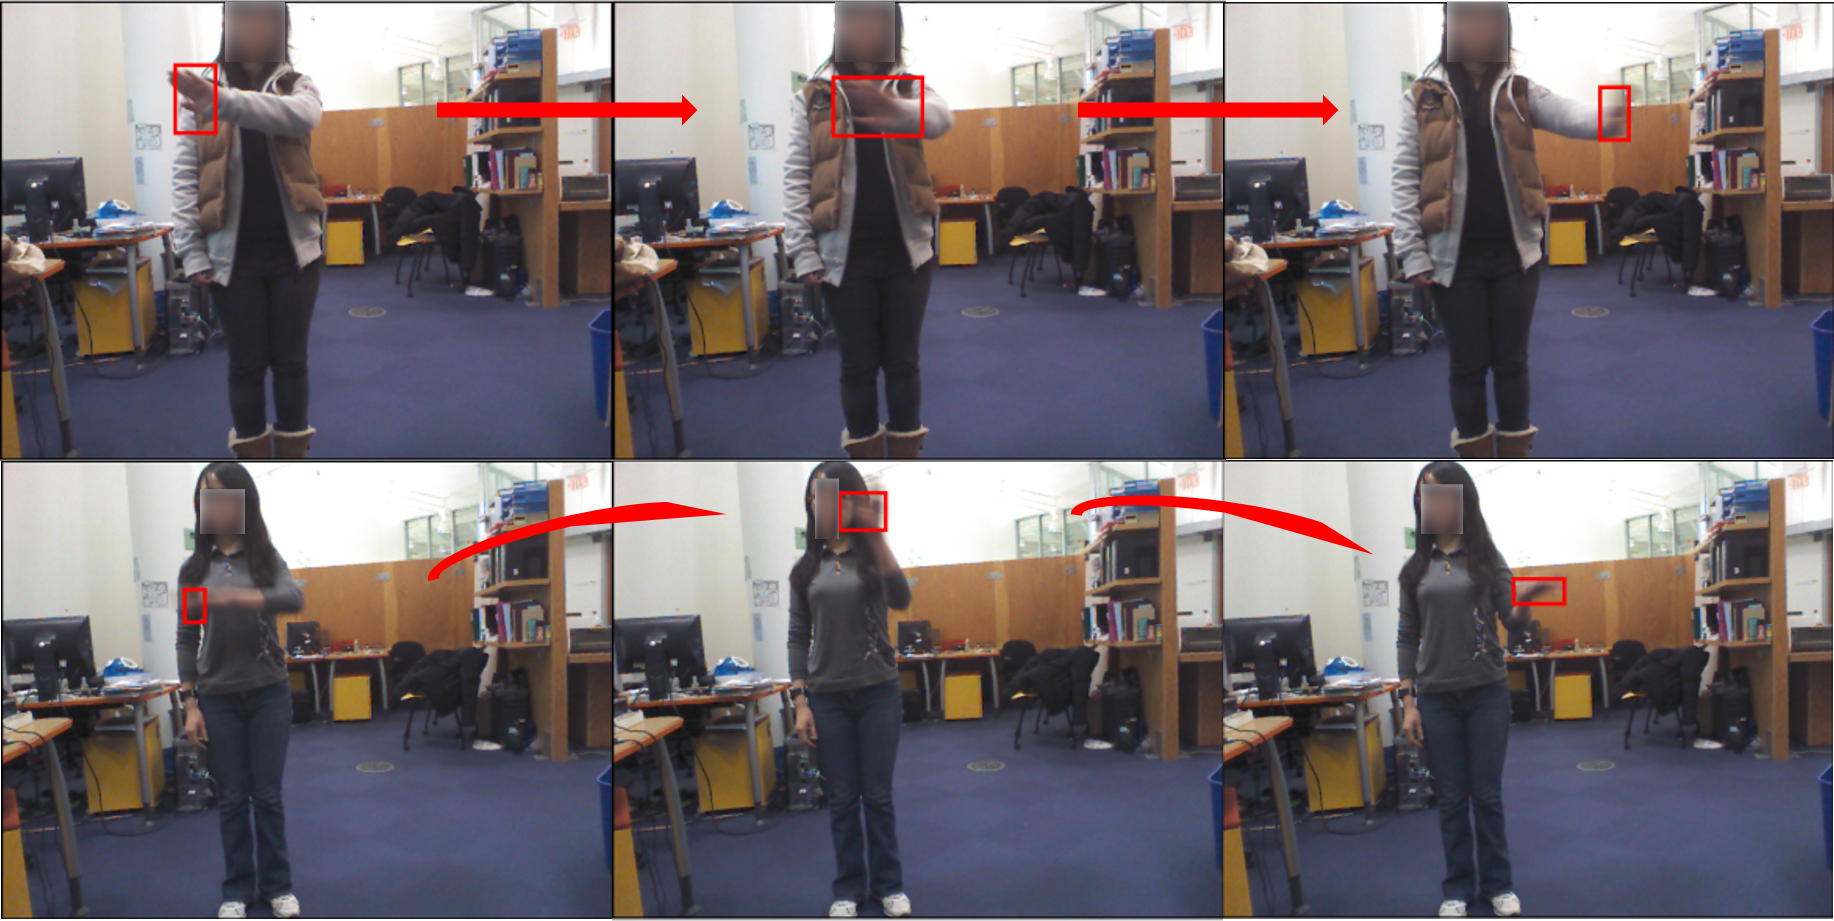
\includegraphics[width=\textwidth]{figures/compare_swipe_right.png}
\caption{Differences between participants for the same swipe right gesture. 
The first row shows that a user does the Swipe Right gesture in a straight
horizontal path with a Palm Up pose; the second row shows that another user
does the same gesture in a curve path with less distinct poses.}
\label{fig:compare-swipe-right}
\end{figure}

\subsection{User Preferences}\label{sec:preferences}
We did a survey with the participants on questions that can influence
gesture interface design. Below are the aggregated results:
\begin{itemize}
  \item User differences: As an example to show user differences, we asked
  the participants how they would prefer to do the Circle gesture. 54\%
  of them prefer doing the Circle gesture in clockwise direction, 15\% in
  anti-clockwise direction, and 31\% do not care.
  \item Predefined gestures versus user defined gestures: 90\%
  of the participants prefer to be able to define their own gestures if necessary while 10\% of them prefer to follow prefined
  gestures completely. No one prefers to use a system without any predefined
  gestures either.
  \item How to define gestures: 80\% prefer defining a gesture by 
  performing it themselves; no one prefers to
  define gestures solely via rules written in terms of positions and directions
  of movement of the hands.
  However 20\% prefer to be able to do both.
  \item Number of repetitions per gesture for training: 50\% are willing to give a
  maximum of 4 -- 6 examples, 40\% are willing ot give 1 -- 3 examples, and 10\%
  are willing to give more than 13 examples. So the average maximum is about 5
  repetitions.
  \item Number of gestures for an application: 80\% think 6--10 gestures are
  appropriate and easy to remember for a given application, while 20\% prefers 1
  -- 5 gestures, giving an average of 7 gestures.
  \item Intuitiveness of the gesture vocabulary for PowerPoint presentation:
  the average score is 4 out of 5 where 5 is very intuitive.
\end{itemize}

\subsection{Implications for a Gesture Interaction Interface}
Based on the observation of the large variation in gesture execution among
users and small variations within users, and the fact that a majority of
participants prefer defining their own gestures if they do not like the
predefined gestures, I suggest that it is more important to optimize user
dependent recognition and user adaptation. As no one prefers to define their own
gesture at the very beginning, it also means that having a reasonable predefined gesture set and
basic user independent model for recognition will be useful too.

Recognition methods based on examples will allow users to train models of their
own gestures easily. We also need to develop methods that
require relatively few training examples and fast training speed.

\section{ChAirGest Dataset}
ChAirGest dataset~\cite{Ruffieux2013} is a publicly available
dataset\footnote{\url{https://project.eia-fr.ch/chairgest/Pages/Download.aspx}}
for the ongoing open challenge on Multimodal Mid-Air Gesture Recognition for
Close
HCI\footnote{\url{https://project.eia-fr.ch/chairgest/Pages/Scoreboard.aspx}}.
Although the dataset only has path gestures, it has other interesting features
which are relevant for evaluating the methods in this thesis:
\begin{itemize}
  \item It has data from both a Kinect sensor and IMU sensors, allowing me to
  evaluate the generalizability of my methods for different sensor input and
  compare recognition performance for different combinations of sensor input. 
  \item It has ground truth labeling of
  pre-stroke, nucleus and post-stroke phases. Few datasets have gesture phase
  labeling. This dataset allows me to evaluate my gesture phase segmentation method.
  \item It represents the scenario where a person sits in front of a
  desk working on a computer. Because of the absence of the full body and the
  presence of the distracting foreground (the desk), the Kinect skeleton
  tracking is less robust. This allows me to evaluate my salience based hand
  tracking method in the case where the skeleton tracking fails.
  \item It contains three different rest poses selected according to common user
  positions when sitting in front of a computer: ``hands on the table'' when
  working/typing, ``elbows on the table, hands joined under chin'' when thinking
  and ``hands on the belly'' when watching a movie. These variations, which
  closely mimic the reality, present challenges to hand tracking, as well as to
  gesture phase detection as the pre-stroke and the post-stroke are
  affected the rest positions.
  \item It contains non-gestures mainly as transitions between rest poses, and
  hence, can be used to evaluate gesture spotting.
\end{itemize}

\subsection{Gestures}
The dataset contains a vocabulary of 10 one-hand/arm gestures focusing on close
HCI (Table~\ref{tab:chairgest-vocab}). The vocabulary has been chosen to present
a range of difficulties, including variations in
paths, hand rotations, and hand poses.
Some gestures have overlapping paths but different hand poses, and this promotes
algorithms using fusion from multiple sensors.

\begin{table}[tbh]
\centering
\begin{tabular}{|l|l|}
\hline
\thead{\#} & \thead{Name of gesture} \\
\hline
1 & Shake Hand \\
\hline
2 & Wave Hello \\
\hline
3 & Swipe Right \\
\hline
4 & Swipe Left \\
\hline
5 & Circle Palm Rotation \\
\hline
6 & Circle Palm Down \\
\hline
7 & Take From Screen \\
\hline
8 & Push To Screen \\
\hline
9 & Palm Down Rotation \\
\hline
10 & Palm Up Rotation \\
\hline
\end{tabular}
\caption{ChAirGest gesture vocabulary.}
\label{tab:chairgest-vocab}
\end{table}

The dataset contains 10 participants, each doing 4 recording sessions with 2
different lighting conditions (dark and normal). In a recording session, the
participant performs once each gesture class for each resting posture. The full
corpus contains $10P\times (2L \times [2S \times 10G \times 3R]) = 1200$
gesture occurrences, where $S$ = subject, $L$ = lighting condition, $S$ =
session, $G$ = unique gesture, and $R$ = resting posture. Only three fourths of
the corpus (3 recording sessions from each participant) is publicly available
and the remaining is used for judging. Hence, in the actual dataset I use, there
are 900 gesture occurrences.

\subsection{Recording Setup}
The participant sits on a chair in front of a desk as if working on a computer.
He/she wears 4 Xsens IMUs attached under his/her clothes on his/her shoulder, arm, wrist and hand.
A Kinect for Windows records the scene from the top of a computer screen with a
30\textdegree downward angle.

\subsection{Data Formats}
The Kinect binary format contains the RGB and the depth streams along with the
3D skeleton representation at 30Hz acquired using the official SDK. Each Xsens IMU
provides information in: linear acceleration, angular acceleration,
magnetometer, Euler orientation and orientation quaternion at 50Hz.

\subsection{Performance Metric}\label{sec:chairgest-metric}
The challenge uses a combination of existing event-based metrics and a novel
time-based metric to evaluate performance. 

The two event-based metrics are
precision and recall, which are combined to compute an $F_1$ score\footnote{See
Appendix~\ref{app:fmeasure} for details}.
Precision is to the number of correctly detected events divided by the number of returned events and recall 
is to the number of correctly detected events divided by the number of
events in the ground truth \cite{Ruffieux2013}. Let
$t_{gt\_start\_nucleus}$ and $t_{gt\_stop\_nucleus}$ be the ground truth start time and stop time of a gesture nucleus respectively,
and let $t_{alg\_start\_nucleus}$ and $t_{alg\_stop\_nucleus}$ be the
corresponding timings returned by a recognition algorithm for the same gesture.
A detected gesture event is correct only if the label of the gesture is
correct and the timings satisfy the following condition
\begin{align*}
|t_{gt\_start\_nucleus} - t_{alg\_start\_nucleus}| &< 0.5\times
(t_{gt\_stop\_nucleus} - t_{gt\_start\_nucleus}) \quad \text{\&\&} \\
|t_{gt\_stop\_nucleus} - t_{alg\_stop\_nucleus}| &< 0.5\times
(t_{gt\_stop\_nucleus} - t_{gt\_start\_nucleus})
\end{align*}
Figure~\ref{fig:true-positive} shows an example comparing the results from two
algorithms. Even though both of them have correct labels for the detected
gesture nucleus, the result from Algorithm 1 is not considered correct because
the time discrepancy is larger than the allowed tolerance, which is half of the
ground truth duration of the gesture nucleus.

\begin{figure}[tbh]
\centering
\includegraphics[width=0.7\textwidth]{figures/true_positive.png}
\caption{Even though the gesture nucleus label detected by Algorithm 1 is
correct (SL stands for ``swipe left''), the start time difference from the
ground truth is too large (larger than half of the ground truth nucleus
duration), and hence, it is not considered as a correct detection. The detection
from Algorithm 2 is considered correct.}
\label{fig:true-positive}
\end{figure}

The time-based metric is used to measure the gesture spotting performance and
the accuracy of temporal segmentation. The metric is named \textit{Accurate
Temporal Segmentation Rate} (ATSR) and represents a measure of the performance
in terms of accurately detecting the start and stop timings of all correctly
detected gesture nuclei. The ATSR is computed as follows: for each correctly detected gesture
occurrence, the \textit{Absolute Temporal Segmentation Error} (ATSE) is computed
according to Equation~\ref{eqn:atse}; the ATSR metric is computed for a
particular sequence with $n$ correctly detected gestures according to
Equation~\ref{eqn:atsr}.
\begin{align}
ATSE &= \frac{|t_{gt\_start\_nucleus} - t_{alg\_start\_nucleus}| +
|t_{gt\_stop\_nucleus} - t_{alg\_stop\_nucleus}|}{t_{gt\_stop\_nucleus} -
t_{gt\_start\_nucleus}} \label{eqn:atse} \\
ATSR &= 1 - \frac{1}{n}\sum_{i=1}^nATSE(i)
\label{eqn:atsr}
\end{align}

The final single metric used by the challenge is the combination
of $F_1$ score and ATSR shown in Equation~\ref{eqn:perf}, which is of the same
form as the $F_2$ metric and correspondingly weighs $F_1$ more than ATSR. This
is because the recognition of gestures remains more important.
\begin{align}
\text{Perf} &= (1 + 2^2)\times \frac{ATSR\times F_1}{2^2\times ATSR +
F_1} \\
 &= 5\times \frac{ATSR\times F_1}{4\times ATSR + F_1}\label{eqn:perf}
\end{align}

\subsection{Evaluation Protocol}
All evaluations based on the ChAirGest dataset reported in this thesis use user
independent training and testing. The results are the average of 3-fold
cross-validation.

\chapter{Hybrid Performance Metric}
It is important to have metrics that can accurately evaluate and compare
performance of different algorithms for a given task domain, and important 
to recognize that a metric that is good for one task, is not
necessarily appropriate for another task. 

\section{Existing Methods for Error Scoring}
Gesture recognition can be considered a sub-domain of human activity
recognition. Two basic units of comparison are typically used in this field
-- frames or events:

\textit{Scoring Frames.} A \textit{frame} is a fixed-length,
fixed-rate unit of time. It is often the smallest unit of measure defined by the system \cite{ward11}, and in such cases approximates continuous time.
For example, in our case, a frame is a data frame consisting of RGB data, depth
data and skeleton data from the Kinect sensor at 30 FPS. If there is ground
truth for each frame, each frame can be assigned to one of: true positive
(TP), true negative (TN), false positive (FP) or false negative (FN). Commonly
recommended frame-based metrics include: true positive rate (TPR $= \frac{TP}{TP
+ FN}$), false positive rate (FPR $= \frac{FP}{TN + FP}$), precision
($\frac{TP}{TP + FP}$).

\textit{Scoring Events.} An \textit{event} is a variable duration sequence of
frames within a continuous time-series.  It has a start time and a stop time.
Given a test sequence of $g$ known events, $E = [e_1, e_2, \ldots, e_g]$, a
recognition outputs $h$ return events, $R = [r_1, r_2, \ldots, r_h]$. There is
not necessarily a one-to-one relation between $E$ and $R$. A comparison can
instead be made using alternative means such as dynamic time warping
(DTW)~\cite{berndt94} or edit distances~\cite{guyon13}. An event can then be
scored as either correctly detected (C), falsely inserted (I), or deleted
(D)~\cite{ward11}. Event scores can be summarized
by precision ($\frac{C}{h}$), and recall
($\frac{C}{g}$).

\section{Shortcomings of Conventional Performance Characterization}
Either frame-based or event-based metrics 
alone may not be adequate for evaluating a real-time continuous gesture recognition system handling different types of gestures. We illustrate this using examples from related work.

Both the ChaLearn Gesture Challenge 2012~\cite{guyon13} and the Multimodal
Gesture Recognition Challenge 2013~\cite{escalera2013} use the Levenshtein edit
distance\footnote{\url{http://en.wikipedia.org/wiki/Levenshtein_distance}},
$L(R, E)$, between the ordered list of recognized events ($R$) and the ground
truth events ($E$) to evaluate performance. However, such event-based metrics
that ignore the timing offset errors are inadequate to identify true positives
in sequences. For example, in Figure~\ref{fig:edit-distance}, both Algorithm 1
and Algorithm 2 would have the same score using their metric. However, Algorithm
1 is in fact worse because the recognized event B is mistakenly considered as a
true positive in the minimum edit distance calculation, and the number
of mistakes should be 3.
Consider a real-time application, if the user does gesture A, it cannot be considered correct if the
system classifies it as gesture B.

\begin{figure}[tbh]
\centering
\includegraphics[width=0.8\textwidth]{figures/edit_distance.png}
\caption{Considering events as an ordered list without timing information does
not give a fair comparison for recognition performance. Applying the edit
distance score used in the challenges, both algorithms have 2 mistakes. However if
we consider the timing of the recognition, Algorithm 1 would have 3 mistakes.}
\label{fig:edit-distance}
\end{figure}

Song et al.~\cite{song12} and Morency et al.~\cite{morency07} used frame-based
metrics to evaluate their continuous gesture recognition systems. Frame-based
metrics consider timing inherently, but there are
artifacts, such as fragmenting and merge errors~\cite{ward11} in the results
that cannot be captured by this type of metrics. For example, in
Figure~\ref{fig:fragment}, Algorithm 1 has a higher frame-based TPR. However,
depending on the application, Algorithm 2 can have a better performance. Suppose we cast this example into a concrete scenario of a gesture-controlled presentation application, 
if the user does a ``swipe left'' gesture, using Algorithm 1, the system would
respond three times and change the slides three times; while using Algorithm 2,
the system would respond one time which is the desired outcome. The same
argument can also be made for merge errors (see Figure~\ref{fig:merge}). This
scenario shows that frame-based evaluation is less relevant for gestures
requiring discrete responses.

\begin{figure}[tbh]
\centering
\includegraphics[width=0.8\textwidth]{figures/fragment.png}
\caption{Even though Algorithm 1 has a higher true positive rate, it has more
fragmenting errors. For certain applications, Algorithm 2 would have a better
performance.}
\label{fig:fragment}
\end{figure}

\begin{figure}[tbh]
\centering
\includegraphics[width=0.8\textwidth]{figures/merge.png}
\caption{Even though Algorithm 1 has a higher true positive rate, it has more
merge errors. For certain applications, Algorithm 2 would have a better
performance.}
\label{fig:merge}
\end{figure}

There are situations where frame-based metrics are more relevant than
event-based metrics as well. Consider the same recognition results in
Figure~\ref{fig:fragment}, but this time gesture A is the ``point'' gesture
requiring continuous frame-by-frame response from the system (e.g., the system
shows a point cursor moving around according to where the user points at). In this case,
Algorithm 1, having a higher frame-based TPR, would have
better performance.

\section{Hybrid Performance Metrics}\label{sec:metrics} 
The examples in the previous section demonstrate the requirement of a hybrid
performance evaluation system. I believe that all three types of information -- frames, events and
timings -- are relevant for a real-time activity/gesture recognition system,
and should be included in the metric.
More importantly, as different categories of activities/gestures require
different kinds of responses from the system, it is necessary to identify
which metric is appropriate for which category of activities/gestures:  the event-based metric is
appropriate for discrete \textit{flow} gestures and the frame-based metric is
appropriate for continuous \textit{flow} gestures.

There are previous works that consider
hybrid metrics. Ruffieux et al.
combined a time-based metric with an event-based metric (see
Section~\ref{sec:chairgest-metric}). They included timing offset errors
explicitly in the metrics, but they did not consider frame-based metric. Ward et
al.~\cite{ward11} proposed a comprehensive scheme to combine both frame and
event scoring, but they did not consider how the different types of metrics are
relevant for different categories of activities.

The following section explains the details of the hybrid performance metric I
propose.

\subsection{Metric for Discrete Flow Gestures}
For discrete \textit{flow} (DF) gestures, the system responds at the end of the
nucleus phase, therefore the evaluation should be event-based. Let
$T_{{\text{gt\_start\_pre}}}$ be the ground truth start time of the pre-stroke phase and
$T_{{\text{gt\_stop\_post}}}$ be the ground truth stop time of the post-stroke
phase.
A recognized event is considered a TP if the time of response ($T_{\text{response}}$) 
occurs between $T_{{\text{gt\_start\_pre}}}$ and $T_{{\text{gt\_stop\_post}}} +
0.5\times(T_{{\text{gt\_stop\_post}}} -
T_{\text{gt\_start\_pre}})$.
We allow some margin for error because there can be small ground truth timing errors\footnote{Pre-stroke and post-stroke
timings are used because there may not be ground truth timings for nucleus
phases, such as in the YANG dataset. Manual labeling of the start and stop
timings of nucleus phases may be too time consuming.}.
Once a TP event is detected, the corresponding ground truth event is not
considered for further matching, so that multiple responses for the same gesture
(fragmenting errors) will be penalized. We then can compute event-based
precision, recall and $F_1$ score for DF gestures:
\begin{align}
\text{precision}^{\text{DF}} &=\frac{\text{\# TP DF events}}{\text{\# recognized
DF events}}
\\
\text{recall}^{\text{DF}} &=\frac{\text{\# TP DF events}}{\text{\# ground truth
DF events}} \\
F_1^{\text{DF}} &= 2\cdot \frac{\text{precision}^{\text{DF}} \cdot
\text{recall}^{\text{DF}}}{\text{precision}^{\text{DF}} +
\text{recall}^{\text{DF}}}
\end{align}

For discrete \textit{flow} gestures, we also define a Responsiveness Score (RS)
as the time difference in seconds between the moment when the system responds and the moment when the hand goes to a rest
position or changes gesture. Let $N_{TP}$ be the number of true positives, then
\begin{align}
RS = \frac{\sum_{i = 1}^{N_{TP}}T_{{\text{gt\_stop\_post}}} -
T_{\text{response}}}{N_{TP}}
\end{align}
A positive score means the responses are before the end of the post-strokes,
hence higher scores are better.

\subsection{Metric for Continuous Flow Gestures}
For continuous \textit{flow} (CF) gestures, the system responds frame by frame,
so it is more appropriate to use frame-based evaluation. For all the frames that are
recognized as continuous gestures, we can compute the number of TPs by
comparing them with the corresponding frames in the ground truth. Then, we can
compute frame-based precision, recall and $F_1$ score for all the frames
corresponding to CF gestures:
\begin{align}
\text{precision}^{\text{CF}} &=\frac{\text{\# TP CF frames}}{\text{\# recognized
CF frames}}
\\
\text{recall}^{\text{CF}} &=\frac{\text{\# TP CF frames}}{\text{\# ground truth
CF frames}}\\
F_1^{\text{CF}} &= 2\cdot \frac{\text{precision}^{\text{CF}} \cdot
\text{recall}^{\text{CF}}}{\text{precision}^{\text{CF}} +
\text{recall}^{\text{CF}}}
\end{align}


The average of the two $F_1$ scores can give an overall indication of the
performance of the system.

\chapter{Hand Tracking}

\section{Kinect Sensor}
The depth sensor data from the Kinect is quite noisy. For a static scene, the
average absolute pixel difference from the RGB camera is about 0.6\% of the maximum value (8
bits), while the average absolute depth difference per pixel is about 4.2\%
(347.89mm) of the maximum value (13 bits).

The random error of depth measurements increases quadratically with increasing distance from the 
sensor and ranges from a few millimeters at 0.5m distance to about 4cm
at the maximum range of 5 meters \cite{khoshelham2011}.

With default range, the depth sensor has a normal range limit of about 0.8m -
4m.

\begin{figure}[h]
\centering
\includegraphics[width=\textwidth]{figures/kinect_sensor_range.png}
\caption{Kinect depth sensor range \cite{microsoft-kinect}.}
\end{figure}

\section{Hand Tracking for Tabletop}
\subsection{System Setup}
The custom tabletop structure includes four $1280\times1024$ pixel projectors 
(Dell 5100MP) that provide a $2560\times2048$ pixel resolution display. The
display is projected onto a flat white surface digitizer (GTCO Calcomp DrawingBoard V), 
which uses a stylus as an input device. The digitizer is tilted 10 degrees down 
in front, and is placed at 41in (104cm) above the floor, following FAA's design 
standard to accommodate the $5^{th}$ through $95^{th}$ percentiles of 
population. The projected displays were mechanically aligned to produce a single 
seamless large display area. The graphics card used is AMD
Radeon\texttrademark{TM} HD 6870 and the operating system used is Ubuntu 11.10.

\begin{figure}
  \centering
  \subfigure[] {
	\includegraphics[width=0.4\textwidth]{figures/setup1.png} 
  }
  \subfigure[] {
  	\includegraphics[width=0.4\textwidth]{figures/setup_close.png}
  }
  \caption{System setup.} \label{fig:setup}
\end{figure}

One Kinect motion sensor by Microsoft is placed above the center of the tabletop
at the same level of the projectors. Figure~\ref{fig:setup} shows the setup. The
Kinect sensor has a RGB camera, a depth sensor and a multi-array microphone.
We use the depth sensor to capture hand motion data because it is
less sensitive to the lighting condition. This is particularly useful for our
projection system. The Dell 5100MP projector uses a spinning color wheel to
modulate the image. This produces a visible artifact on the screen, referred to 
as the ``rainbow effect'', with colors separating out in distinct red, green, 
and blue. At any given instant in time, the image on the screen is either red, or green, or blue,
and the technology relies upon people's eyes not being able to detect the rapid 
changes from one to the other. However, when seen through a RGB camera, the
effect is very obvious, and this can greatly affect hand segmentation if we were to use 
the RGB images. 

The Kinect sensor outputs video at a frame rate of 30Hz. The depth sensing video
stream has a resolution of $640\times 480$ pixels with 11-bit depth value. The
depth value increases as the distance of the object from the sensor increases.
The tabletop surface is about 1.2m away from the Kinect
sensor which allows us to have a relatively good depth resolution. We use the
open source OpenNI framework \footnote{https://github.com/OpenNI/OpenNI} and its
Kinect driver \footnote{https://github.com/avin2/SensorKinect} to get both the depth and RGB data streams.

\subsection{Kinect Calibration}
In order to develop an interactive interface, we need to map the point in the
depth image to the point on the display. We do this by projecting a
checkerboard image on the tabletop display, and placing some wooden blocks at
the corners of the checkerboard image to create the depth differences so that 
the depth sensor can capture these corners (see Figure~\ref{fig:calibration}).
We manually labeled 16 pairs of corresponding points on the display and the depth image. Then we
apply undistortion to the depth image and planar homography to find the mapping.

\begin{figure}[h]
  \centering
  \includegraphics[width=0.5\textwidth]{figures/calibration.png} 
  \caption{Kinect calibration. The darker squares are the wooden blocks. The
  intensity of the gray level image is inversely proportional to the distance
  from the Kinect sensor.}
  \label{fig:calibration}
\end{figure}

Planar homography is a projective mapping from one plane to another. In our
case, we are mapping points on the plane of the depth image to the points
on the plane of the display. To evaluate the result of the calibration, we
obtain a new set of manually labeled corresponding points on the display and the
depth image. We then transform the coordinates of the points on the depth image
to the coordinates on the display using the calibration result, and find the
Euclean distance (error) between the transformed coordinates and the labeled
coordinates of the points on the display. The average errors in the x-axis and
y-axis are 4.3px and 8.9px respectively, which are 0.21cm, and 0.4cm in physical distance of the
projected display. The average width of the index fingertip is about 1.4cm, so
the error is less than 30\% of the width of the fingertip. 

\subsection{Hand Tracking}
The hand tracking process consists of feature detection and parameter estimation. The hand tracking
pipeline consists the following steps:

\begin{enumerate}
  \item Background subtraction
  \item Forelimb and hand segmentation
  \item Fingertips tracking
\end{enumerate}

The following subsections explain in details about these steps. Many of the
computer vision methods we use are based on the OpenCV
\footnote{http://opencv.willowgarage.com/wiki/} library and its Java interface 
JavaCV \footnote{http://code.google.com/p/javacv/}.

\subsubsection{Background Subtraction}
While the background - i.e., the tabletop - is relatively static, there is
still noise from the depth sensor. We use the averaging background method, which
learns the average and average difference of each pixel in the depth image as
the model of the background. The average values are based on the initial 30
frames with no hands in the scene. For the subsequent frames, any value that is 
6 times the average frame-to-frame absolute difference below the average tabletop depth value for that pixel is considered 
foreground because it is closer to the sensor above.

To clean up the background subtracted depth image, we use 1 iteration of
morphological opening to clear out small pixel noise. Morphological opening is a
combination of erosion and dilation. Both erosion and dilation are morphological
transformations. The kernel of erosion is a \textit{local minimum} operator,
while that of dilation is a \textit{local maximum} operator.

\begin{figure}[h]
  \centering
  \subfigure[Without using morphological opening.] {
	\includegraphics[width=0.4\textwidth]{figures/background_subtraction.png} 
  }
  \subfigure[Using morphological opening to clear out small pixel noise.] {
  	\includegraphics[width=0.4\textwidth]{figures/morphology.png}
  }
  \caption{Background subtraction.} \label{fig:setup}
\end{figure}


\subsubsection{Forelimb and Hand Segmentation}
With the cleaned up background subtracted depth image, we find connected
components by finding all contours that are not too small. These components are
considered to be the forelimbs and are approximated with convex hulls and 
bounding boxes. The hand region is at either end of the bounding box depending
on the position of the arm relative to the table.

\subsubsection{Fingertips Tracking}
We base our estimation of the hand model on geometric properties of the
hand. We compute the convexity defects from the convex hull of the forelimb
(Figure \ref{fig:convexity_defects}). From this we can observe that for an
extended finger, it has one convexity defect on each side and the two adjacent sides of the defects form an
acute angle. We iterate through the adjacent convexity defects, and mark the
intersection of those sides that form an angle smaller than a threshold
value as the potential fingertip. We further refine the fingertip position by
searching in the general direction of the finger and finding a sharp change in
the gradient of the depth value.

\begin{figure}[h]
  \centering
  \includegraphics[width=0.4\textwidth]{figures/convexity_defects2.png} 
  \caption{The white triangles are the convexity defects.}
  \label{fig:convexity_defects}
\end{figure}

\subsubsection{Kalman Filter}
We use a Kalman filter to further improve tracking accuracy. The dynamic state
of the fingertip can be summarized by a $4$-dimensional vector, $x_k$, including
two position variables, $x$ and $y$, and two velocities, $v_x$ and $v_y$. The
measurement is a $2$-dimensional vector, $z_k$, of the measured $x$ and $y$ coordinates of the fingertip.

Assuming no external control, the a priori estimate $x_k^-$ of the state is
given by:
\begin{align*}
x_k^- = Fx_{k - 1} + w_k
\end{align*}
$F$ is the $4$-by-$4$ \textit{transfer matrix} characterizing the
dynamics of the system with the following values:

\begin{align*}
x_k = \begin{bmatrix}
	x   \\
	y   \\
	v_x \\
	v_y \end{bmatrix}_k, \quad
F = \begin{bmatrix}
	1 & 0 & 1 & 0 \\
	0 & 1 & 0 & 1 \\
	0 & 0 & 1 & 0 \\
	0 & 0 & 0 & 1 \end{bmatrix}
\end{align*}
assuming constant velocities, and that time is measured in frames.
$w_k$ is the \textit{process noise} associated with random events or forces
that directly affect the actual state of the system. We assume that the 
components of $w_k$ have Gaussian distribution $N(0, Q_k)$ for some $4$-by-$4$ 
covariance matrix $Q_k$. We set the matrix $Q$ with the following values:
\begin{align*}
Q = \begin{bmatrix}
	1 & 0 & 0 & 0 \\
	0 & 1 & 0 & 0 \\
	0 & 0 & 10 & 0 \\
	0 & 0 & 0 & 10 
	\end{bmatrix}
\end{align*}
The larger variance values indicate the greater uncertainty in the velocities as
they may not be constant.

\subsubsection{Evaluation}
We evaluate the accuracy of our fingertip tracking method by comparing the
detected fingertip position with the manually labeled position in a sequence of
video frames. In this first evaluation, only one extended finger is used. Our
method finds all the labeled fingertips and the average error (Euclean distance)
is 5.3px which is about 10mm. In their finger click evaluation, Harrison et al.
reports that their system has an average of 11.7mm offset from the targets. 

Here we want to emphasize that the focus of the thesis is gesture recognition
and finding a hand model that is suitable for gestural input. As a result, we
are not pushing the accuracy of fingertip and click detections to as high as
possible. We also envision that better touch screen hardware will be developed
in the near future with larger size and higher resolution, and hence, touch
detection accuracy can be very high. Our hand model and gesture analysis
framework should be general enough such that it can be easily adapted to
different sensor inputs.

\section{Hand Tracking for Seated Interaction with Vertical Display}
\subsection{Gesture Salience Detection}
Similar to Marcos-Ramiro et al.~\cite{marcos2013}, we define gesture
\textit{salience} as a function of both the closeness of the motion to the
observer (e.g., the camera) and the magnitude of the motion.
There are 4 steps in our method (Figure~\ref{fig:gesture-salience}).

\begin{figure*}[tb]
\centering
\hspace{-0.6em}%
\subfigure[]{
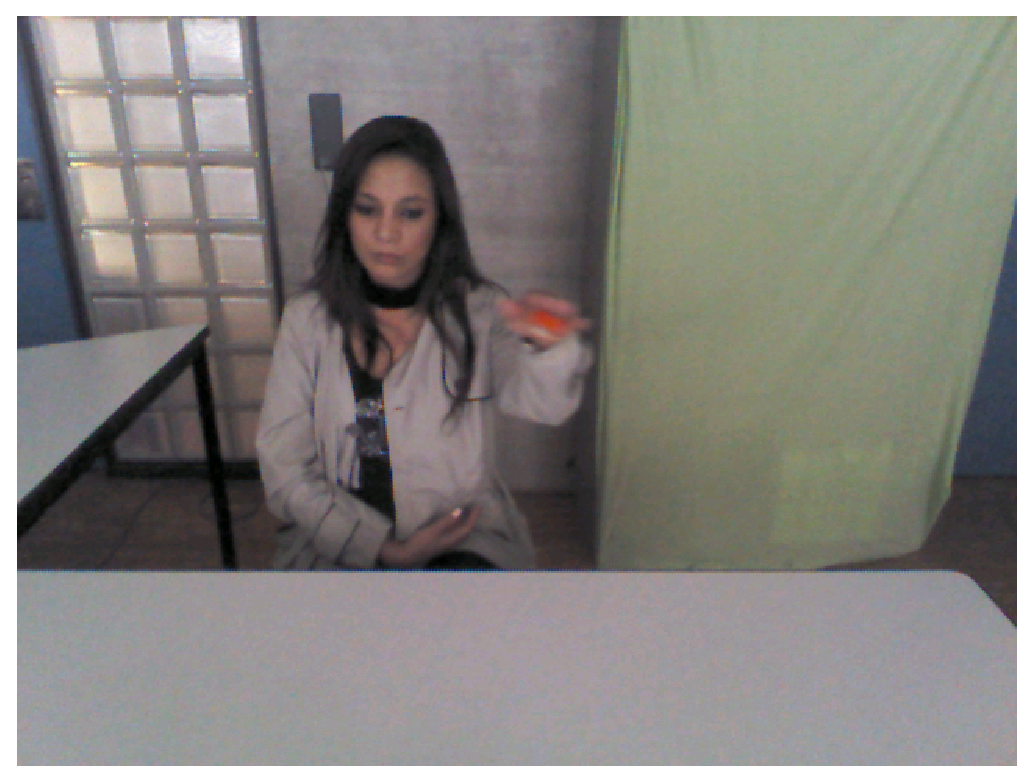
\includegraphics[width=0.19\linewidth]{figures/color.eps}\hspace{-0.6em}%
\label{fig:color}
}
\subfigure[]{
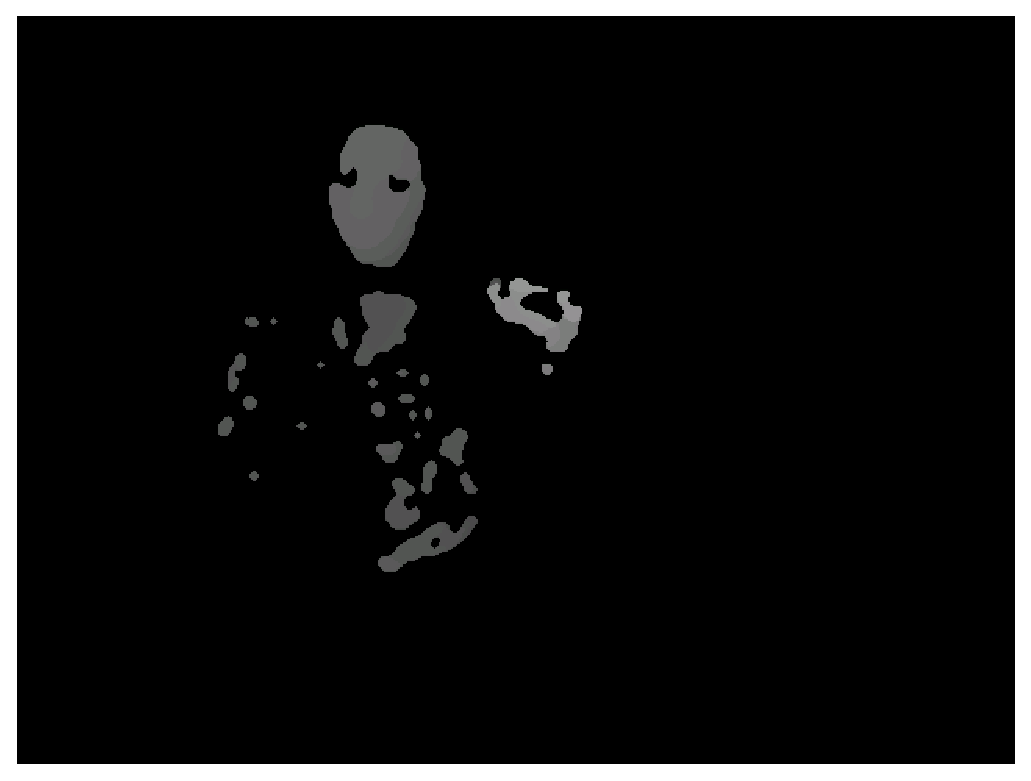
\includegraphics[width=0.19\linewidth]{figures/depth.eps}\hspace{-0.6em}
\label{fig:skin-mask}
}
\subfigure[]{
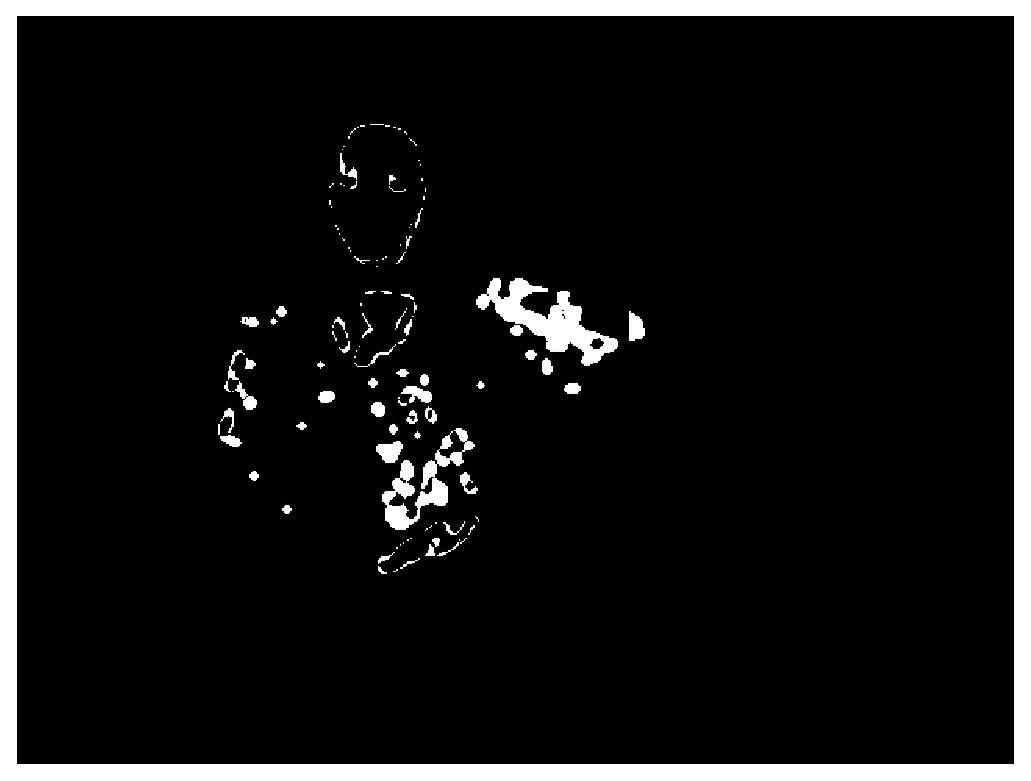
\includegraphics[width=0.19\linewidth]{figures/motion-mask1.eps}\hspace{-0.6em}
\label{fig:motion-mask}
}
\subfigure[]{
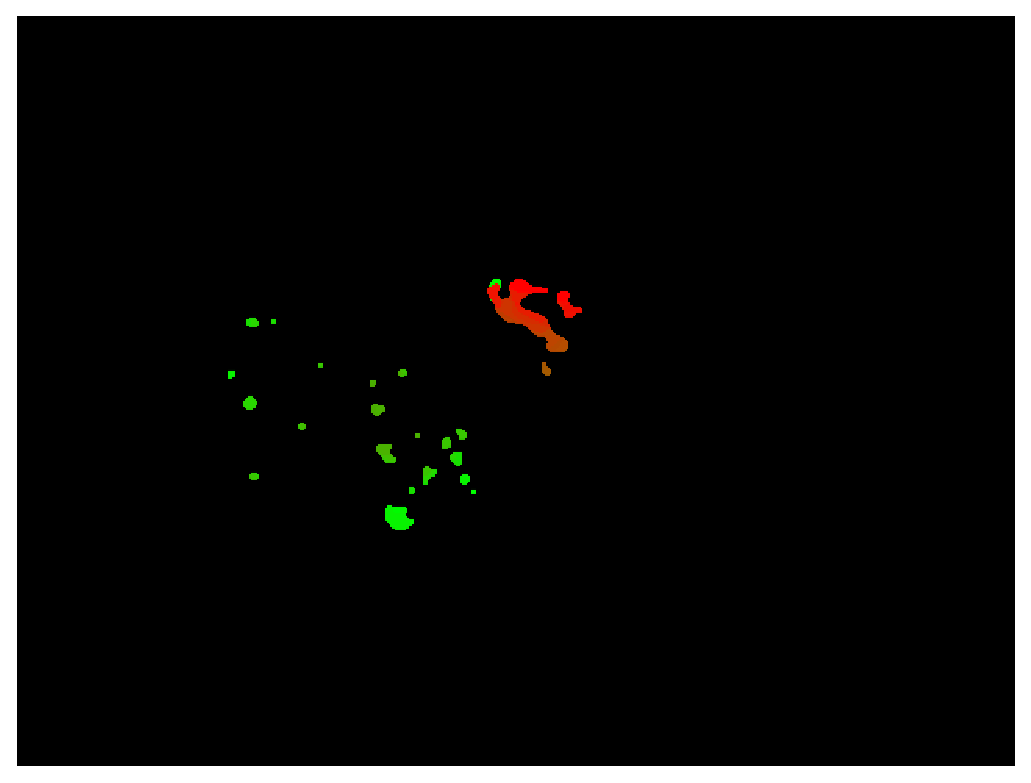
\includegraphics[width=0.19\linewidth]{figures/salient-map.eps}\hspace{-0.6em}
\label{fig:salience}
}
\subfigure[]{
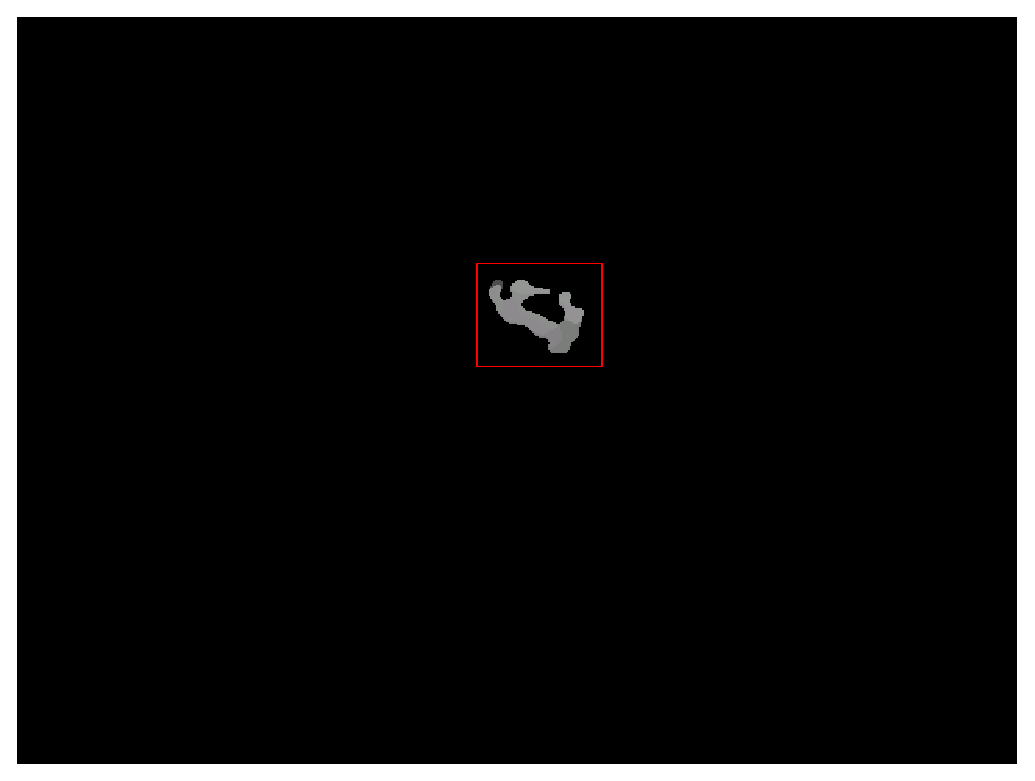
\includegraphics[width=0.19\linewidth]{figures/bounding-box.eps}
\label{fig:camshift}
}
\caption{Gesture salience detection steps: \subref{fig:color} RGB image under low lighting condition;
\subref{fig:skin-mask} depth map $D_t$ filtered by skin and user mask, $M_t^{S\wedge U}$. False detection of skin is due to
the similar colors between clothes and skin; \subref{fig:motion-mask} motion mask,  $M_{t\vee t-1}^M$, indicating moved pixels for time $t$ and $t-1$;
\subref{fig:salience} salience map with red color indicating high probability of the salience;
\subref{fig:camshift} final gesture salience bounding box, $B_t$. (Best viewed in
color. Based on data from ChAirGest corpus~\cite{Ruffieux2013}.)}
\label{fig:gesture-salience}
\end{figure*}

\subsubsection{Skin Segmentation}
We use an off-the-shelf simple skin color detection method to compute a binary skin mask at
time $t$, $M_t^S$, based on the RGB image. We also find the user mask, $M_t^U$ obtained from the Kinect SDK based on the depth image.
We align the two to find their intersection $M_t^{S\wedge U}$, which indicates the user's skin region.

\subsubsection{Motion Detection}
The depth data is first clipped to a maximum value $\text{depth}_\text{max}$ of
2m and then scaled to a value between 0 and 255 (1 byte):

\begin{align*}
\text{scaled} = (\text{depth}_\text{max} -
\text{depth}_\text{clipped}) \times 255 / \text{depth}_\text{max}
\end{align*}

The scaled value is inversely proportional to the depth value.
We compute the motion mask for the current depth frame based on 3 frames. We first filter each
depth frame by the user and skin mask $M_t^{S\wedge U}$, and then
smooth it through a median filter to obtain $D_t$ (Figure~\ref{fig:skin-mask}).
Equation~(\ref{eq:motion-mask}) computes the binary mask, $M_{t\vee t-1}^M$,
indicating pixels whose depth values have changed from time $t-1$ to $t$ (Figure~\ref{fig:motion-mask}).
$D_{t\vee t-1}$ is the absolute difference between $D_t$ and $D_{t-1}$, and $T$ is the threshold operator that filters out small changes in depth value
(with a threshold of 15mm).
To obtain the motion mask, $M_{t}^M$ for time $t$ only, we use $M_{t-1\vee t-2}^M$, the motion mask for $t-1$ and $t-2$ as well (see Equation~(\ref{eq:motion-mask-t}),
 AND and XOR are indicated by $\wedge$ and $\oplus$).
\begin{align}
M_{t\vee t-1}^M &= T(D_{t\vee t-1}) \label{eq:motion-mask} \\
M_{t}^M &= M_{t\vee t-1}^M \oplus (M_{t\vee t-1}^M \wedge M_{t-1\vee t-2}^M) \label{eq:motion-mask-t}
\end{align}

\subsubsection{Salience Map}
We compute histograms of depth values in both $D_t$ and $D_{t\vee t-1}$ and then apply histogram normalization to obtain cumulative distributions $H_t$ and $H_{t\vee t-1}$.
$H_t$ represents the probability of salience given a depth value, while $H_{t\vee t-1}$ represents the probability of salience given
a depth difference value. The lower the depth value or the higher the depth difference value, the higher the salience probability. We use
histogram equalization to reduce the effect of outliers, so that a single large depth value will not suppress the salience probabilities of other depth values.
The salience map (Figure~\ref{fig:salience}) can then be computed for each pixel $(x, y)$:
\begin{align*}
S_t(x, y) = H_t(D_t(x, y)) \times H_{t\vee t-1}(D_{t\vee t-1}(x, y)) \times M_t^M
\end{align*}
The multiplication of the binary motion mask $M_t^M$ allows us to consider only the motion due to the user at $t$.

\subsubsection{Salience Location}
The final step of locating the most salient region in a frame is finding the
contour, $C_t$, from the salience map $S_t$ that has a perimeter greater than
the smallest possible hand perimeter and with the highest average salience for all the pixels inside the contour.

When motion is slow, the motion mask usually indicates the edge of the moving
object. As a result, the center of $C_t$ may not be the center of the moving
object (in our case, the user's hand). Hence, we use 2 iterations of Camshift~\cite{Bradski98} on
the depth image $D_t$ with a starting search location at the center of $C_t$ to refine
the final bounding box, $B_t$, of gesture salience (Figure~\ref{fig:camshift}).

Figure~\ref{fig:compare-skeleton} shows examples of our hand tracking result (red regions).
It is more reliable than the hand joint locations from the Kinect SDK. In the
Experimental Evaluation section (Section~\ref{sec:eval}), we show that using our
salience detection method to extract hand position features gives 3.7\%
absolute increase in gesture recognition F1 score compared to using the hand
joint position from the Kinect SDK.

\begin{figure*}
\centering
\subfigure[]{
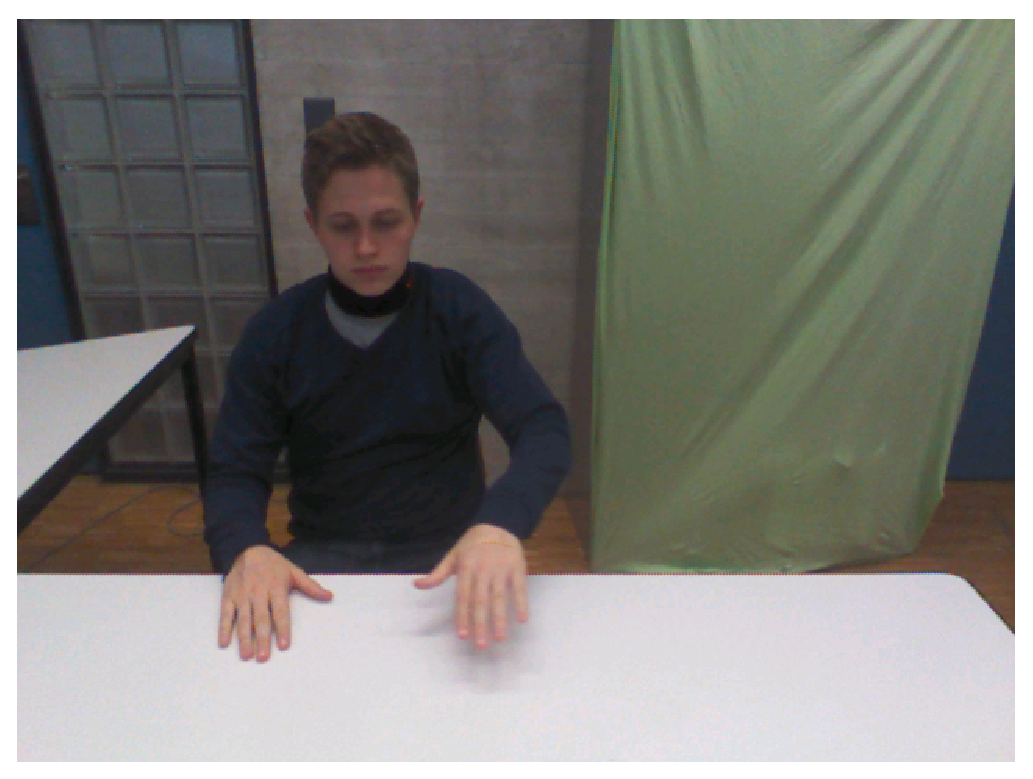
\includegraphics[width=0.23\linewidth]{figures/rotate-color.eps} \hspace{-0.6em}
}
\subfigure[]{
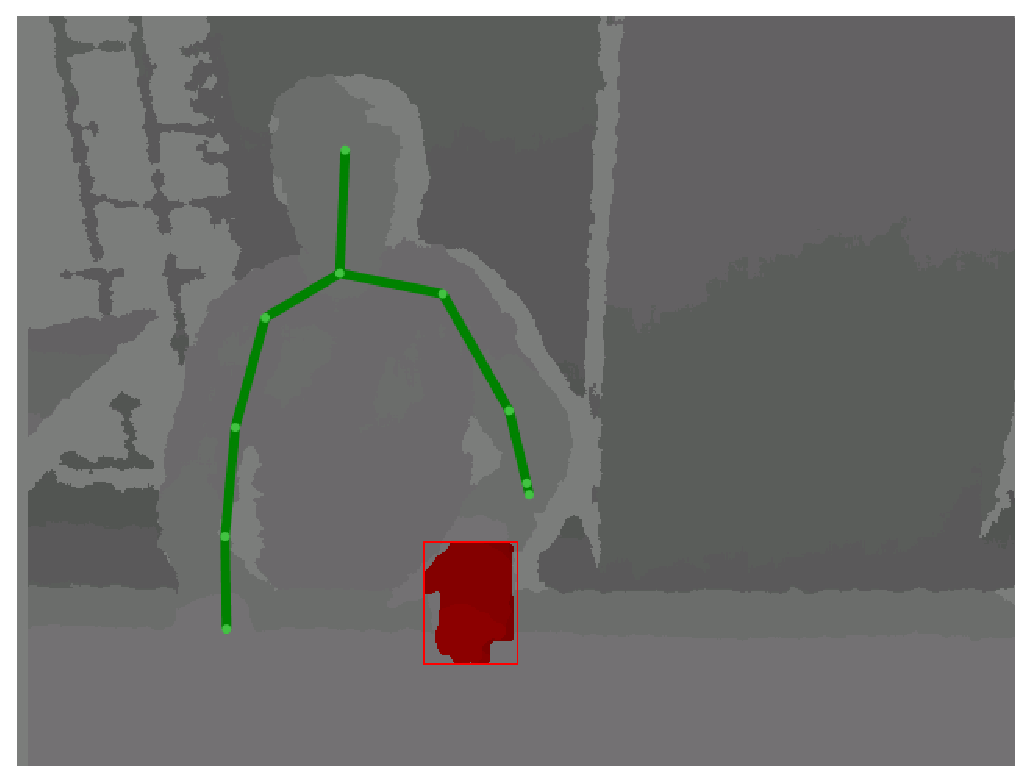
\includegraphics[width=0.23\linewidth]{figures/rotate-depth.eps} \hspace{-0.6em}
}
\subfigure[]{
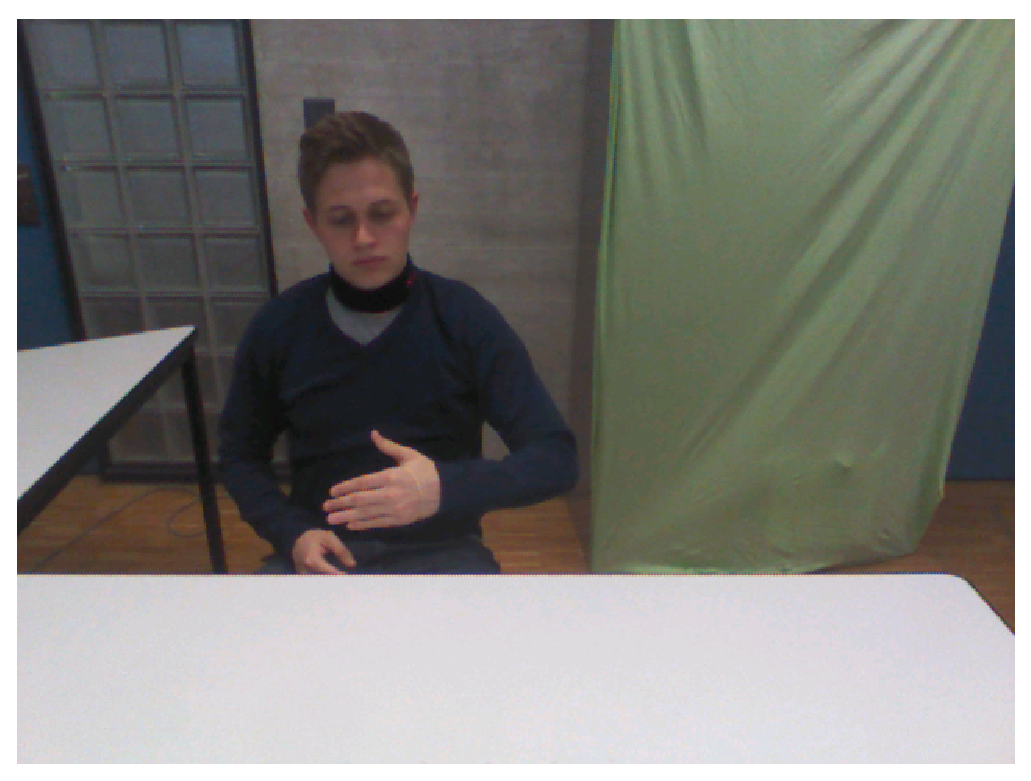
\includegraphics[width=0.23\linewidth]{figures/near-body-color.eps}
\hspace{-0.6em} }
\subfigure[]{
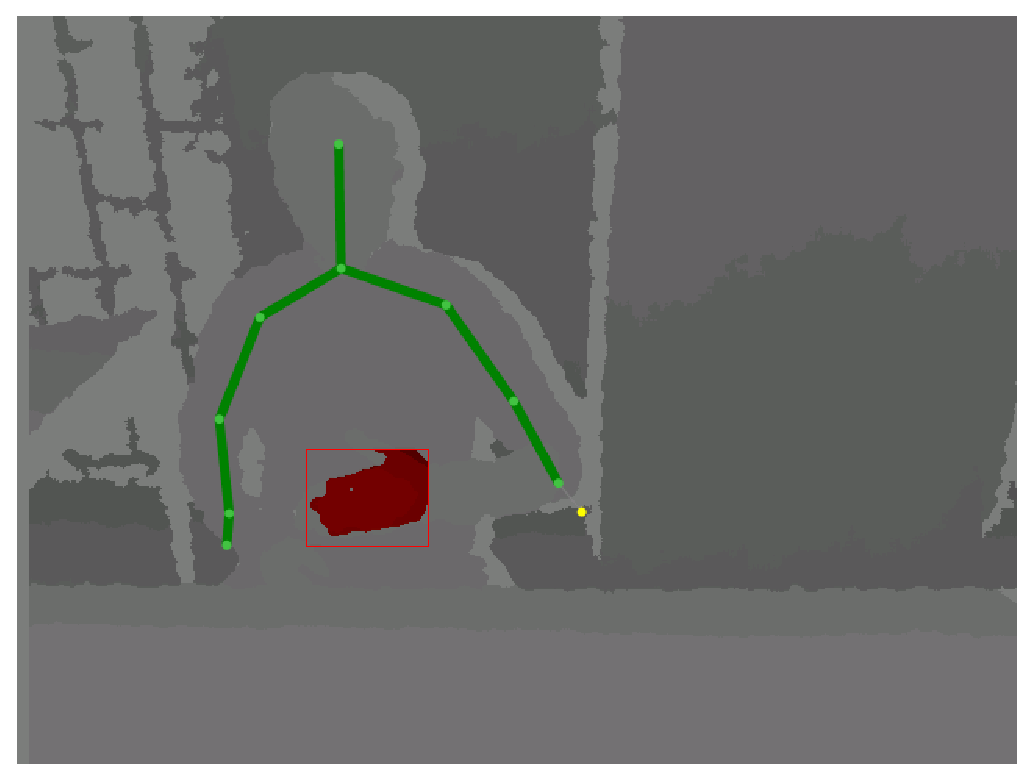
\includegraphics[width=0.23\linewidth]{figures/near-body-depth.eps}
\hspace{-0.6em} }
\caption{Comparison of hand tracking results. Our method (red region) gives more
reliable result on hand tracking compared to the off-the-shelf Kinect software
(green line). (Best viewed in color. Based on data from ChAirGest
corpus~\cite{Ruffieux2013}.)}
\label{fig:compare-skeleton}
\end{figure*}
\chapter{Hand Features and Representations}

Different hand feature representation and encoding methods are compared. The
hand features can be extracted from either color, depth or both images. 
\begin{figure}[t]
  \centering
  \subfigure[Color images] {
	\includegraphics[width=0.45\textwidth]{figures/color_hand.png} 
  }
  \subfigure[Depth images] {
  	\includegraphics[width=0.45\textwidth]{figures/depth_hand.png}
  }
  \caption{$64\times64$ pixel raw image patches of hands.} \label{fig:hand}
\end{figure}

\begin{figure}[t]
\centering
\includegraphics{figures/hand3d.png}
\caption{View of quantized depth data of a hand in 3D.}
\end{figure}

During training, all the features are standardized to have 0 mean and 1 standard
deviation using all the training data before being input to the recognition
module. During testing, the data are standardized using the mean and and
standard deviation from training.

\section{Motion Features}
We use both the Kinect and the Xsens data from the ChAirGest corpus~\cite{Ruffieux2013} to
extract hand motion feature vectors for gesture modeling.

It is relatively easy to obtain features from the Xsens data. We choose to use linear
acceleration (x, y, z), angular velocity (x, y, z) and Euler orientation (yaw, pitch, roll)
from the Xsens unit on the hand to form a 9-dimensional feature vector $\underline{x}_t^{\text{xsens}}$
for every time frame $t$.

From hand tracking using a Kinect sensor, we can extract the position of the
gesturing hand in $(x, y, z)$ coordinates relative to the shoulder center joint to
form a 3-dimensional vector. From this, we can again compute  the 
velocity and and acceleration, all in 3D world coordinates. The feature vector
is computed for each input frame streamed from the sensor to form a sequence of
feature vectors.

Combining the two, we
have a 12-dimensional feature vector $\underline{x}_t = [\underline{x}^\text{kinect}_t, \underline{x}^\text{xsens}_t]$.

It is also useful to apply temporal smoothing on the motion data. In our
real-time system, we apply ``box'' smoothing (i.e., simple and linear smoothing
with equal weight) with a window size of 15 frames on the relative positions of
the gesturing hand.

Figure~\ref{fig:motion-hist-rest} shows the histograms of the standardized $(x,
y, z)$ coordinates of relative position, velocity and acceleration from one user's
data in the YANG dataset. The peak values corresponds to rest positions.
Figure~\ref{fig:motion-hist} shows the histogram of the same data excluding
those from rest position. We can see that the distribution roughly follows
Gaussian or mixture of Gaussians distributions.

\begin{figure}[t]
\centering
\subfigure[]{
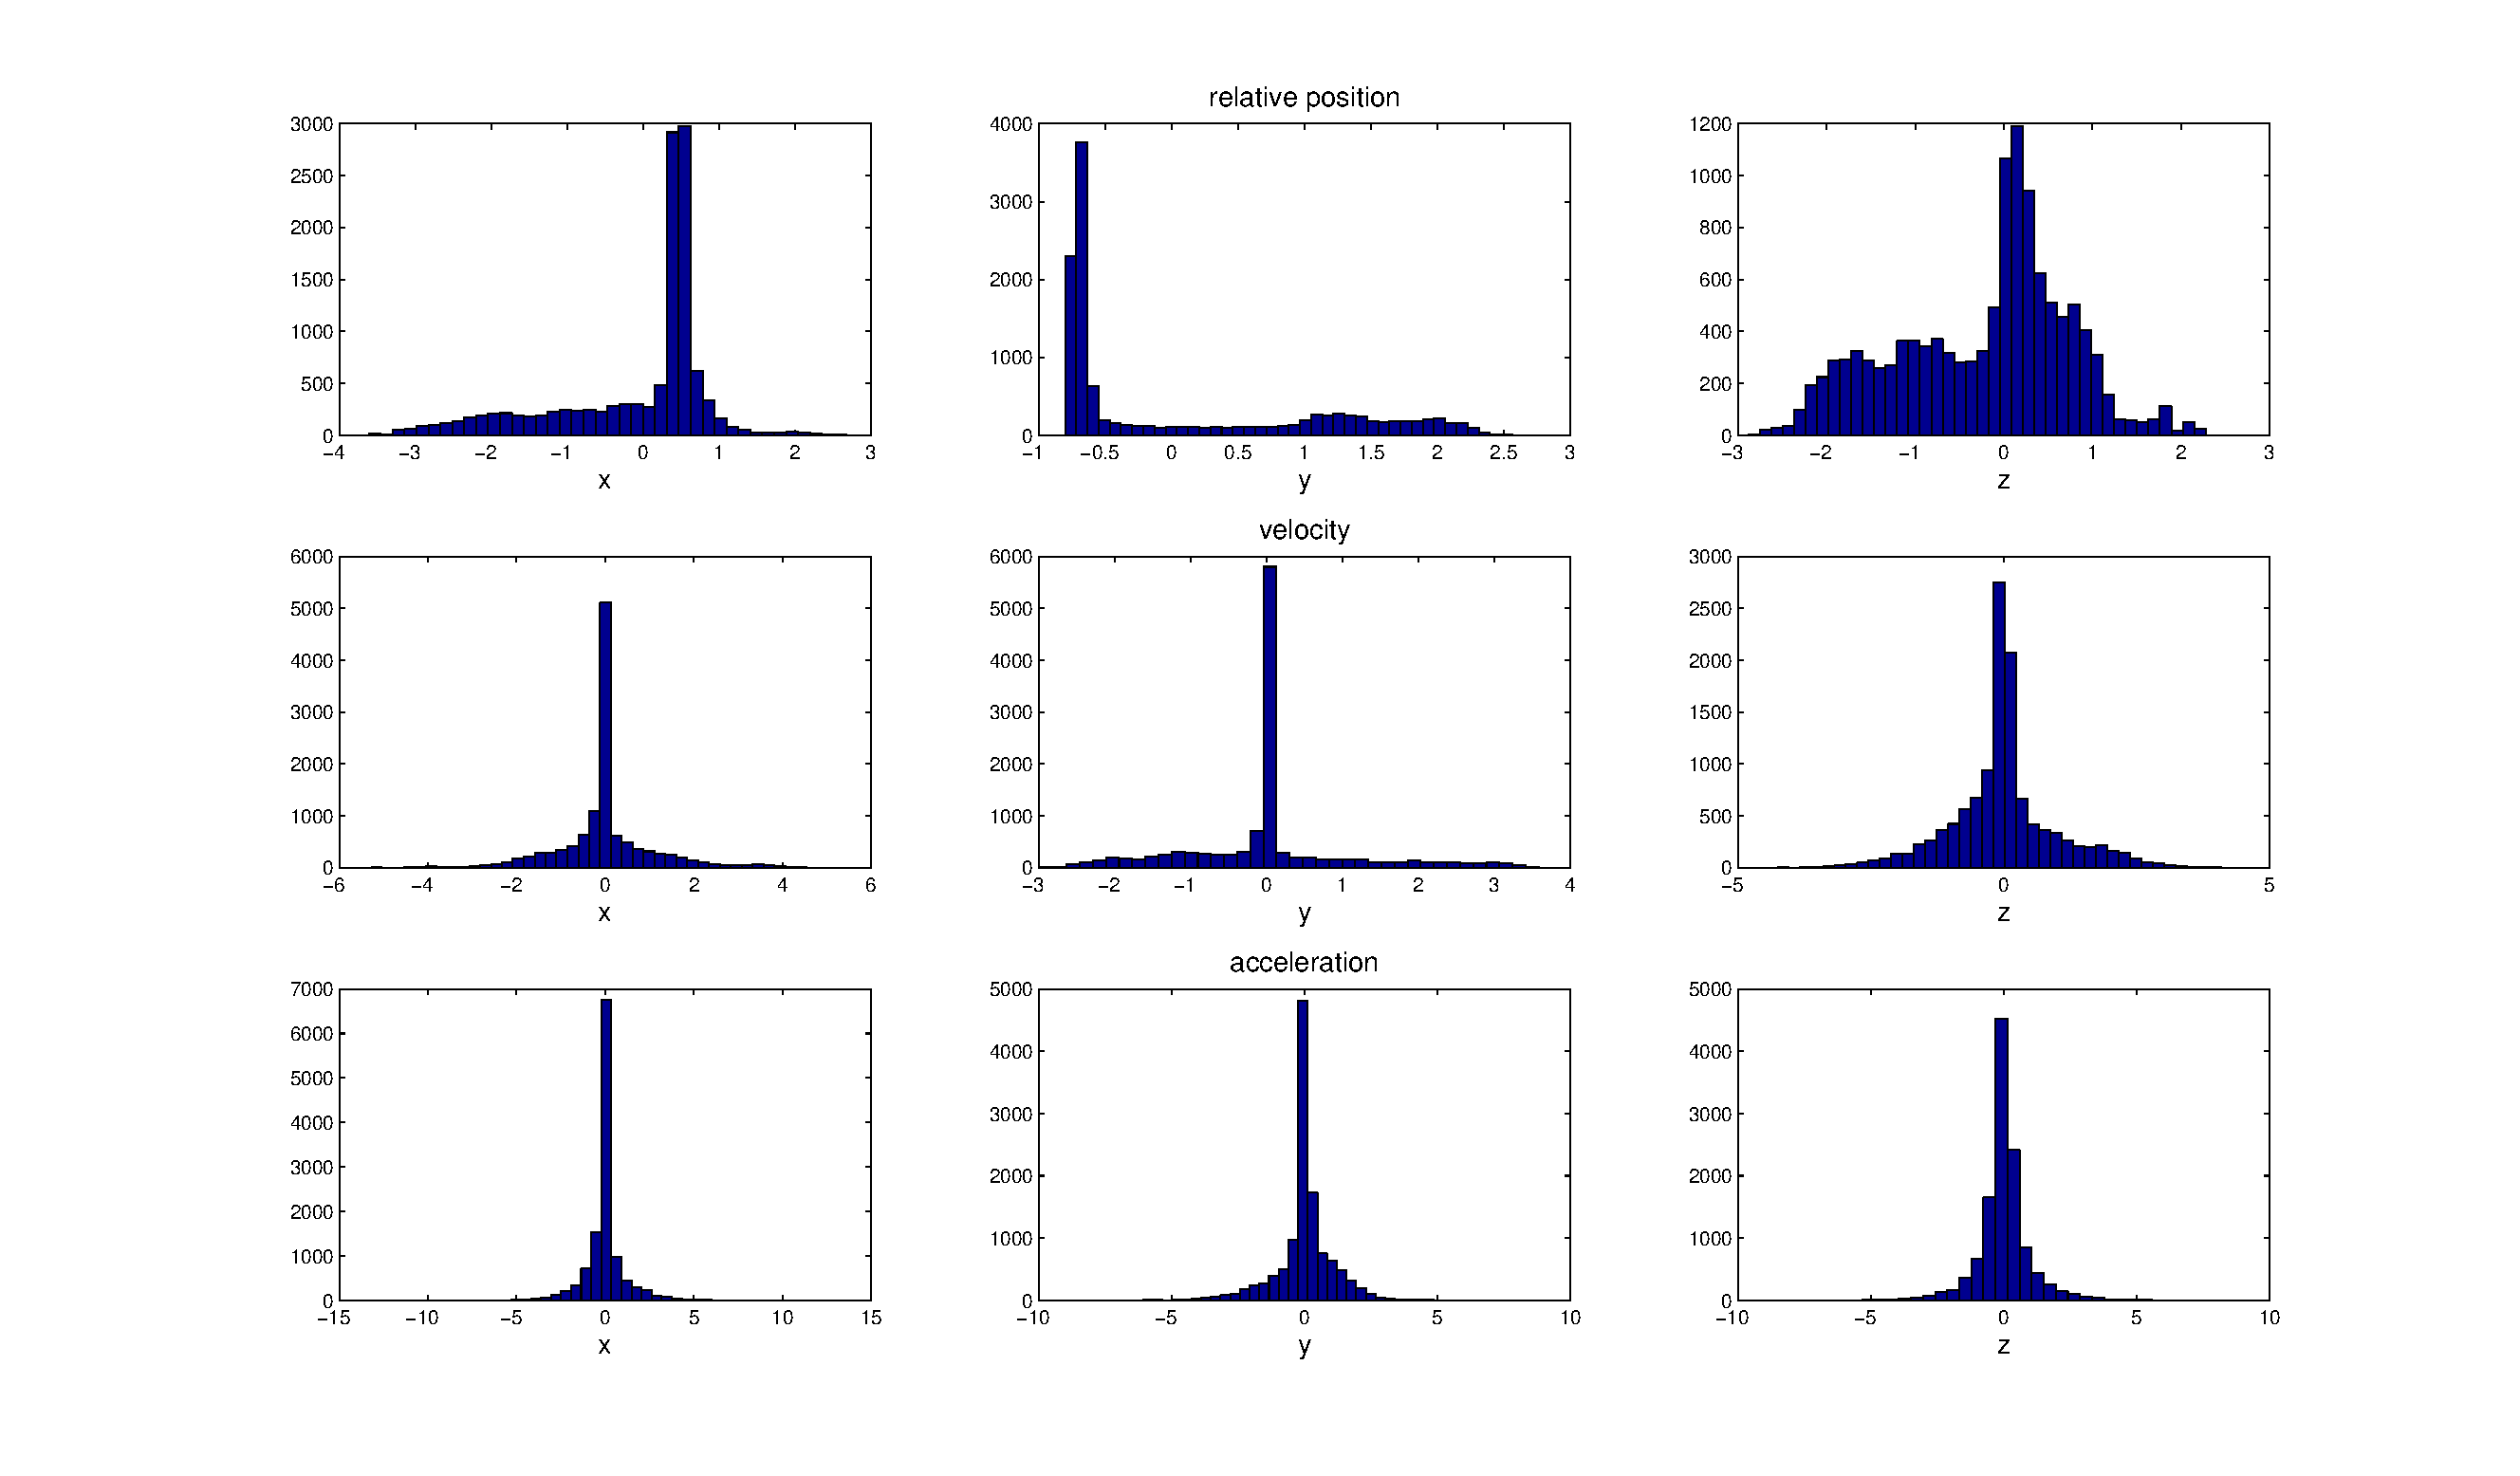
\includegraphics[trim=30mm 15mm 30mm 10mm,
clip, width=\columnwidth]{figures/motion_hist_rest.eps}
\label{fig:motion-hist-rest}
}
\subfigure[]{
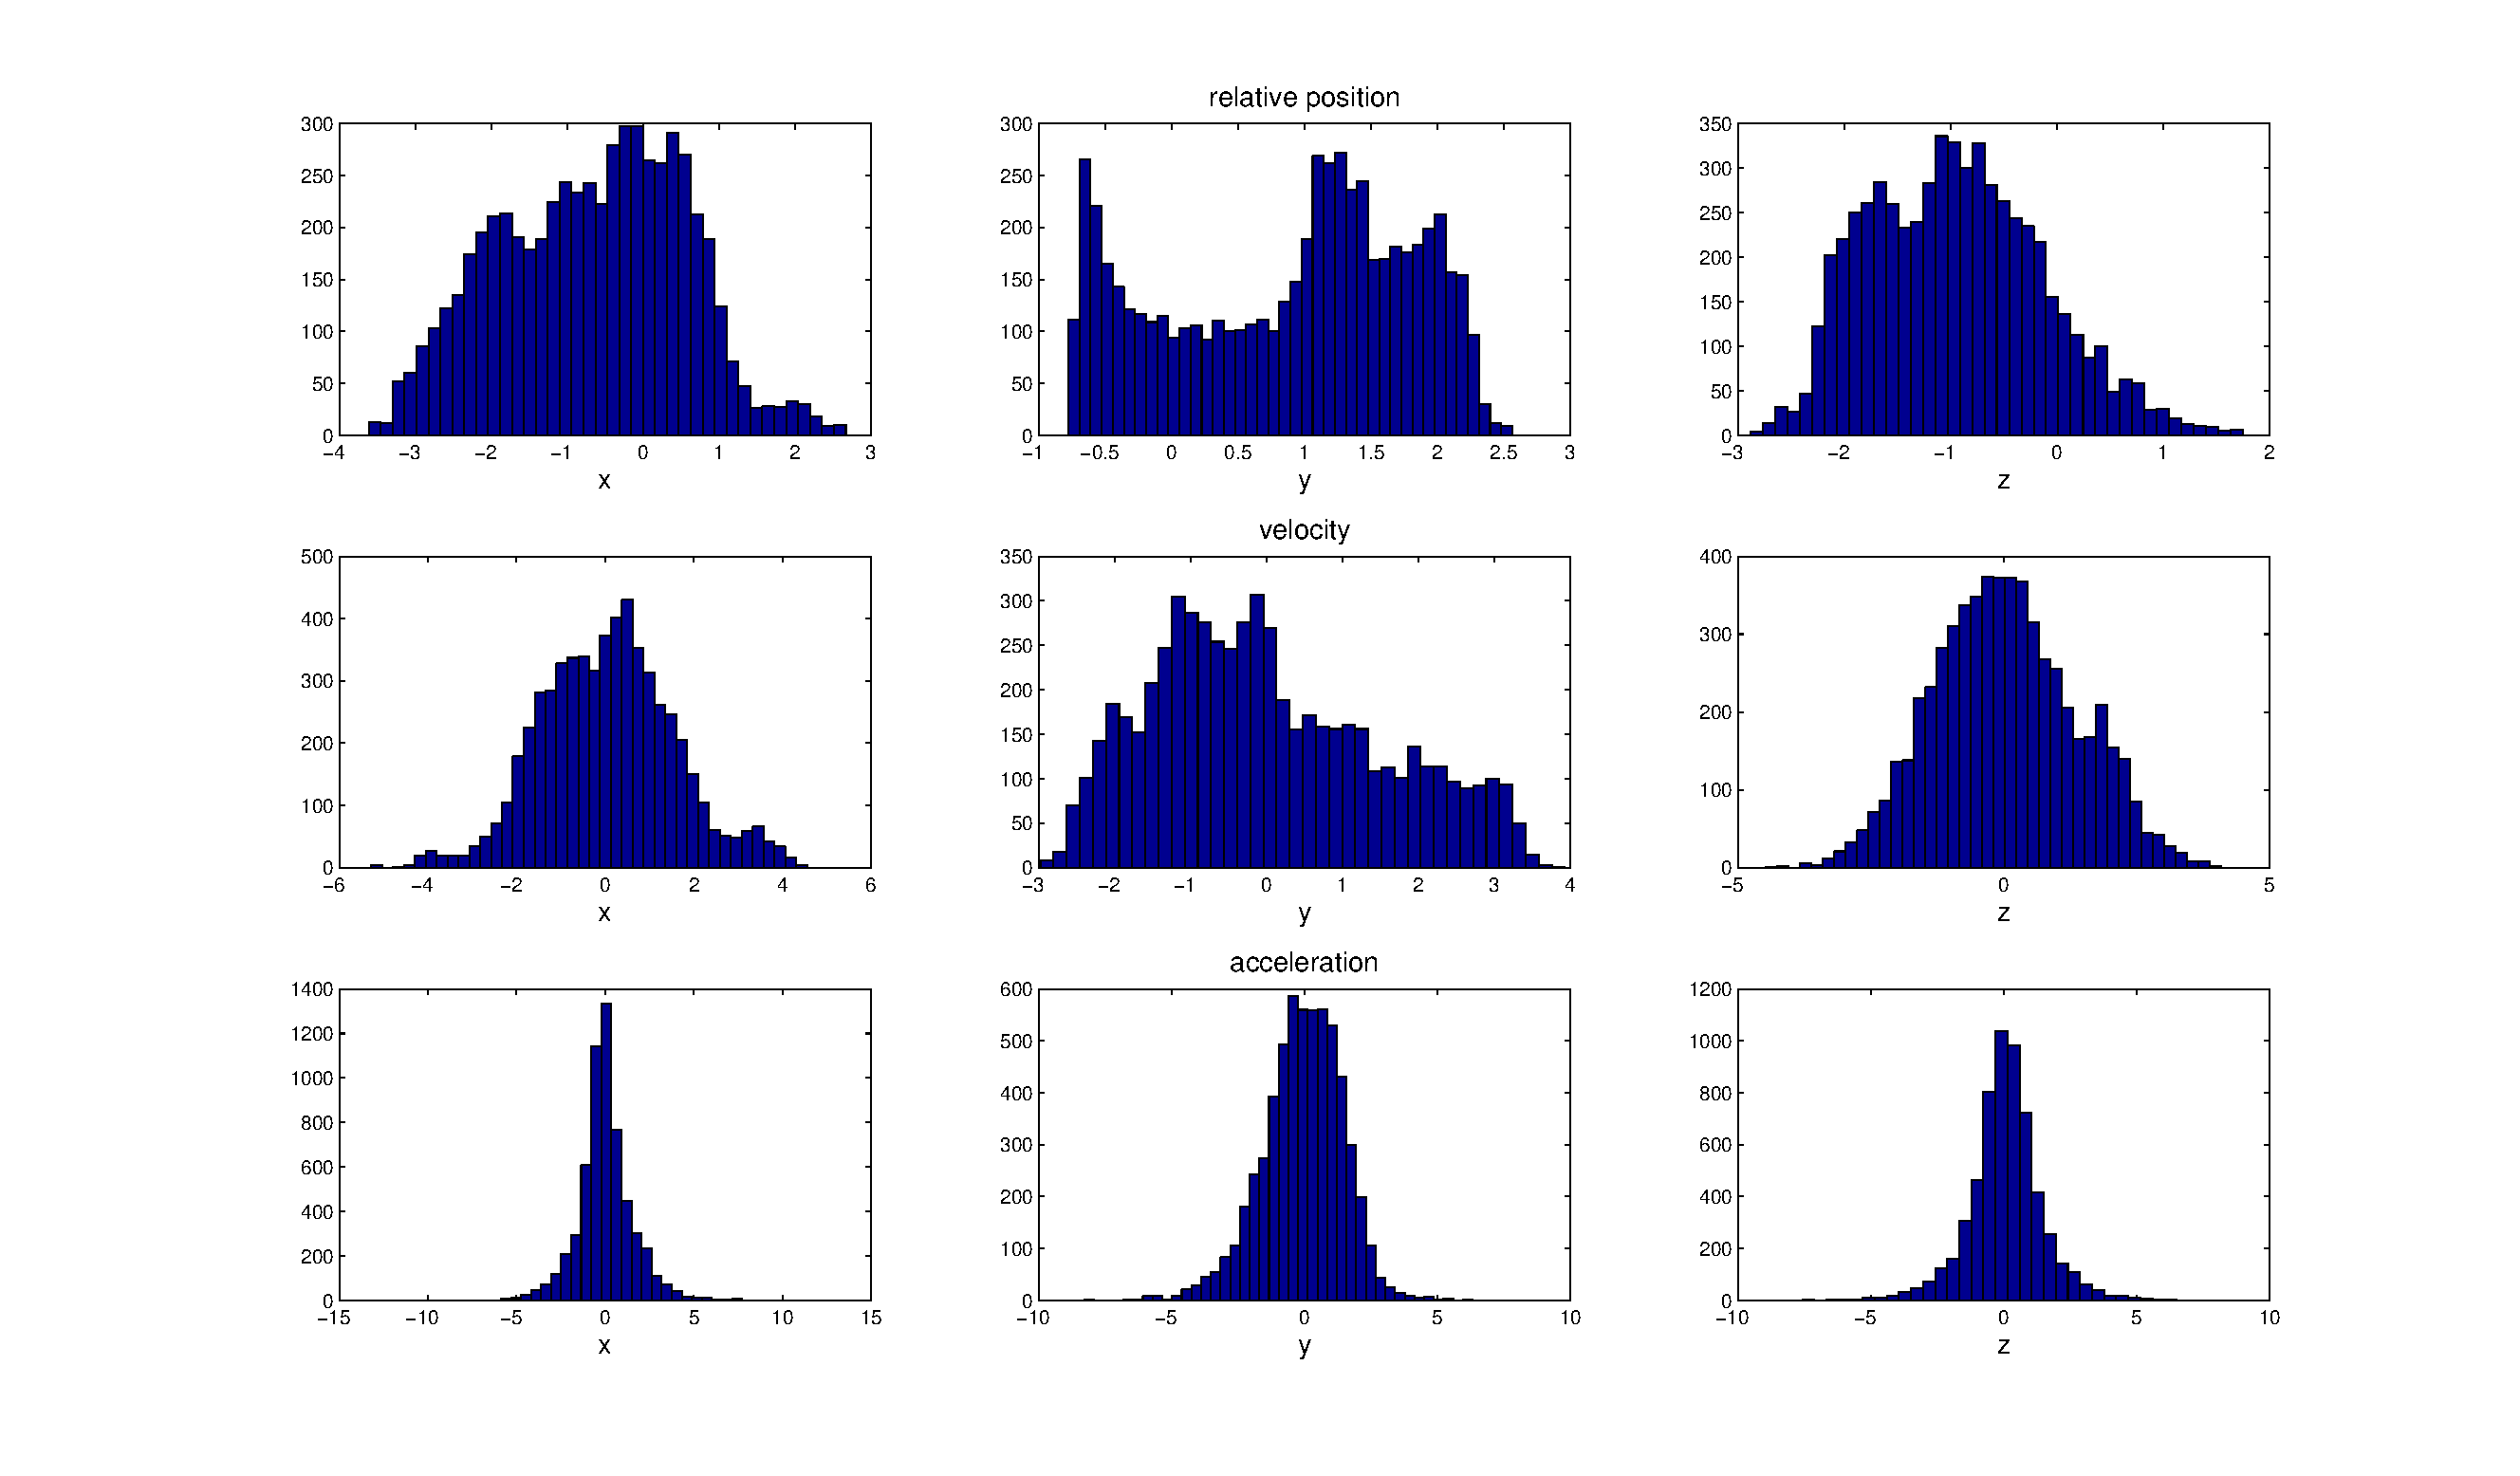
\includegraphics[trim=30mm 15mm 30mm 10mm,
clip, width=\columnwidth]{figures/motion_hist.eps}
\label{fig:motion-hist}
}
\caption{Histograms of motion features.}
\end{figure}

Try Xsens data on hand, quarternion.

\section{Histogram of Oriented Gradients}
For each pixel, the magnitude of gradient is 
\begin{align*}
m = \sqrt{dx^2 + dy^2}
\end{align*}

If an image $I$ has dimensions $m\times n$, the size of the computed feature
vector $H$ is $(m/\text{cell\_size} - fold_per_dim) \times (n/\text{cell\_size}
- fold_per_dim) \times \text{num\_bin}$.

\begin{figure}[h]
  \centering
  \subfigure[Color] {
  \includegraphics[width=0.45\textwidth]{figures/color_denoised_5.png} 
  }
  \subfigure[Depth] {
    \includegraphics[width=0.45\textwidth]{figures/depth_denoised_5.png}
  }
  \subfigure[Color HOG] {
  \includegraphics[width=0.45\textwidth]{figures/color_hog.png} }
  \subfigure[Depth HOG] {
    \includegraphics[trim={0cm 1.5cm 0cm 0cm},
  clip, width=0.5\textwidth]{figures/depth_hog.png}
  }
  \caption{$64\times64$ pixel image patches of hands.} \label{fig:hand}
\end{figure}




\section{SVM for hand pose classification}
SVM for unbalanced data. \cite{ben2010}
If we ignore the  fact that the data is unbalanced, the resultant classifier
will favor the majority class, in this case the ``other'' category. To take this
into account, we can assign different misclassification (SVM soft-margin
constants) to each class. If $n_1$ and $n_2$ are the number of examples in two
classes, 

\begin{align}
\frac{C_+}{C_-} = \frac{n_-}{n_+}
\end{align}

\begin{figure}
\centering
\subfigure[]{
  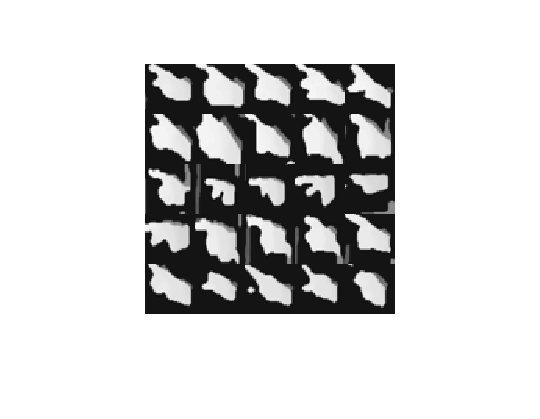
\includegraphics[width=0.5\linewidth,
  trim={0cm 1cm 0cm 0cm}, clip]{figures/point_depth_resize_32_denoise.eps} }
\subfigure[]{
  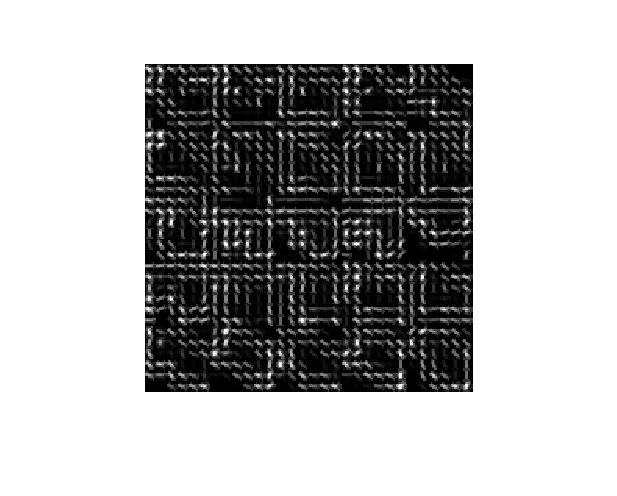
\includegraphics[trim={0cm 1cm 0cm 0cm},
  clip, width=0.45\linewidth]{figures/point_depth_hog.eps} }
\subfigure[]{
  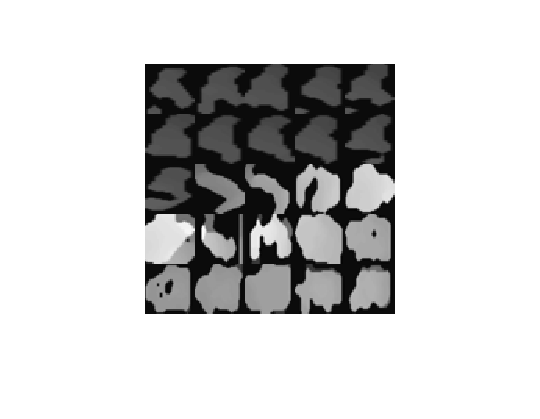
\includegraphics[width=0.5\linewidth,
  trim={0cm 1cm 0cm 0cm}, clip]{figures/other_depth_resize_32_denoise.eps} }
\subfigure[]{
  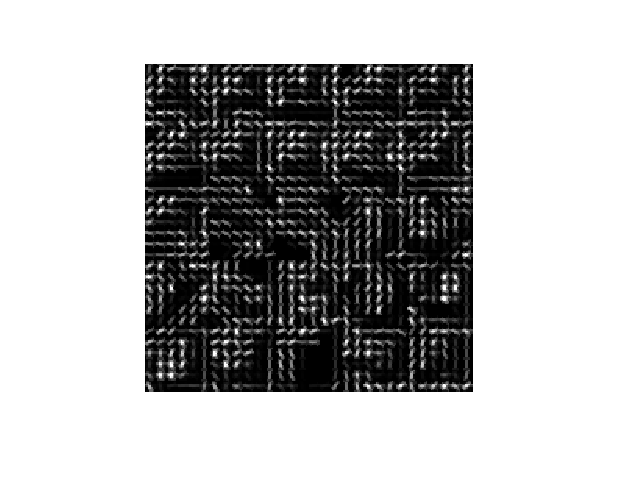
\includegraphics[trim={0cm 1cm 0cm 0cm},
  clip, width=0.45\linewidth]{figures/other_depth_hog.eps} }
\end{figure}

Radial Basis Function (RBF) kernel, use grid search to find best parameters, C =
0.03, $\gamma = 0.5$. Ratio between point pose and other poses is 27 : 73, so
the weight for $C_other$ and $C_point$ is 73 : 27. 

no standardization.

Test accuracy 92.6282\% (289/312) 2-class classfication


\section{Dictionary Learning}

\section{PCA and Sparse PCA}
We use Principal Component Analysis (PCA)~\cite{pca} to reduce the
dimensionality of the HOG features. The number of principal components to use
is determined through cross-validation. For the YANG dataset, we use 15
principal components from the HOG features.

\begin{figure}[t]
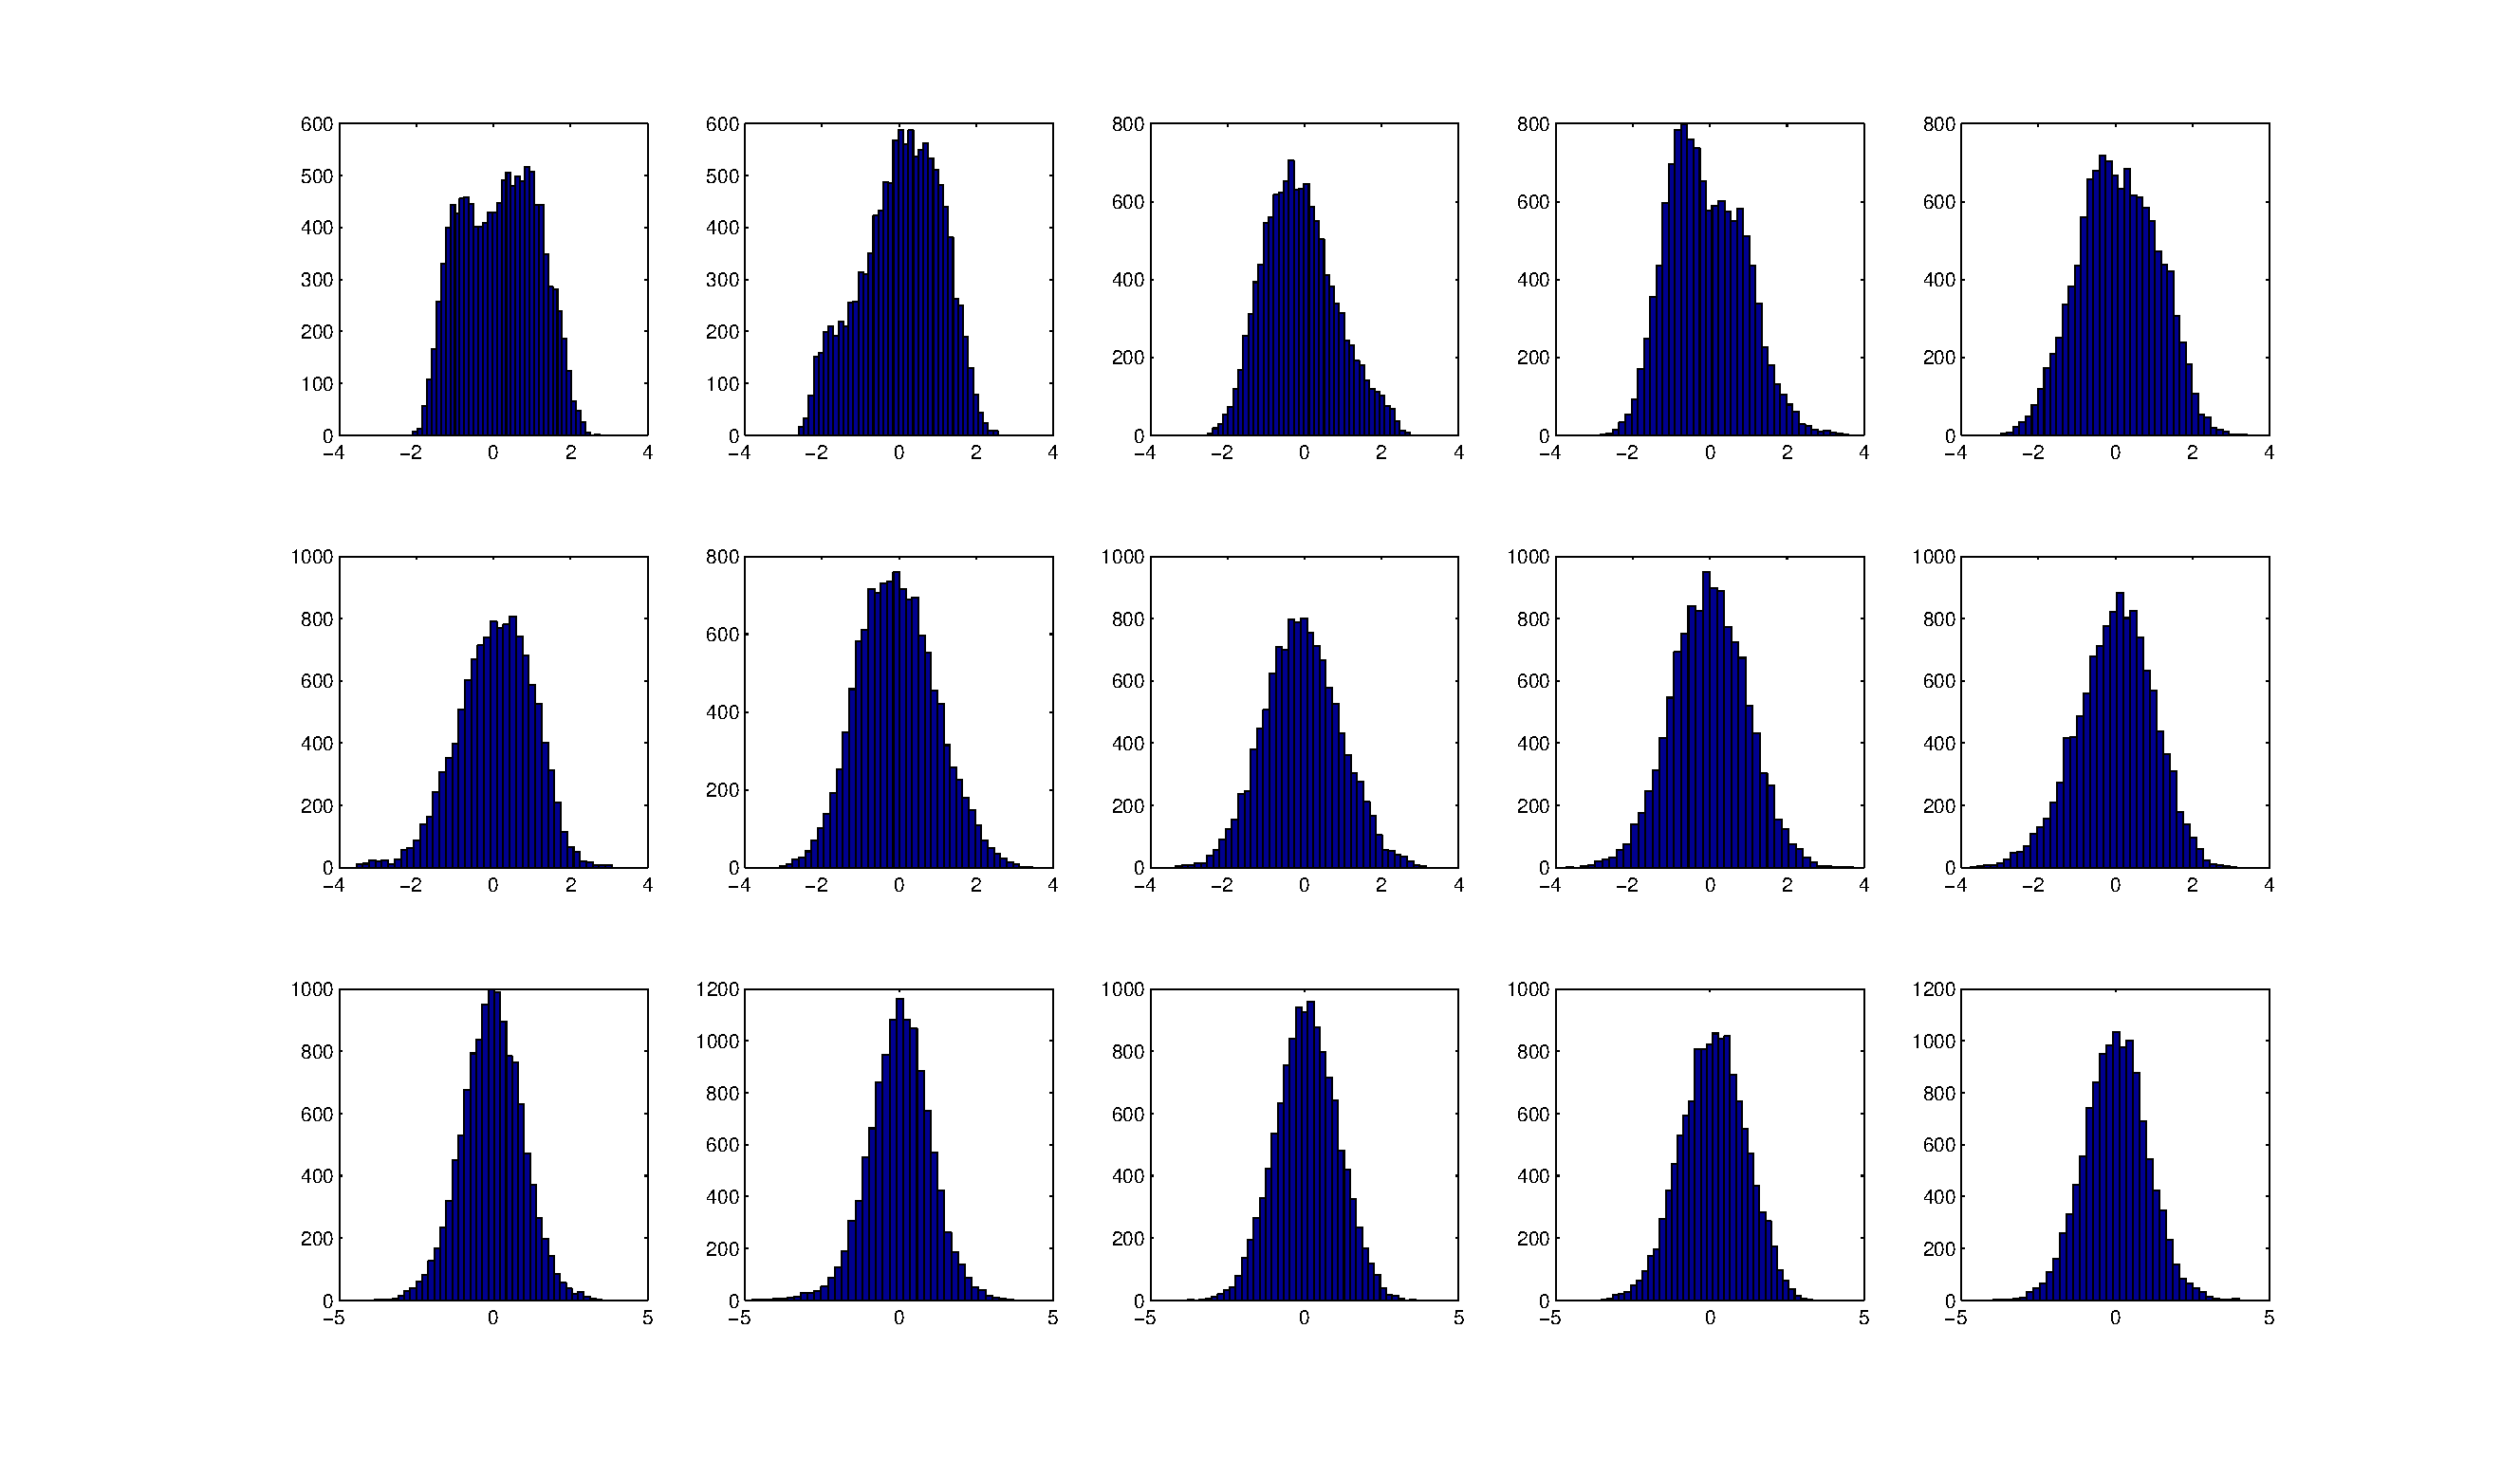
\includegraphics[width=\columnwidth]{figures/hist_pca.eps}
\end{figure}
\begin{savequote}
Apparently the child recognizes speech sounds as patterns of gestures.
\qauthor{Israel Rosenfield, \textit{The invention of memory}}
\end{savequote}
\chapter{Unified Gesture Recognition Framework}

As mentioned in the Chapter~\ref{chap:related} Related Work, most prior works
focus on recognizing one form of gestures: either path or pose gestures.
We could conceivably just combine the two forms by first deciding what
category the gesture is and then apply different recognition methods. However making
decisions too early may not be robust. For example, if the system categorizes
the gestures wrongly, it will be hard to correct that in the later stage. We
could also apply two different methods simultaneously, e.g., compute likelihood
from HMMs for path gestures and compute SVM probability scores for pose
gestures, but it is not clear how these probabilities can be compared for making
final decisions.

As a result, I developed a unified probabilistic framework to handle the two
forms of gestures so that probabilities are comparable. During online
recognition, the system makes soft decisions rather than hard decisions, and
propagates probabilities until a response (decision)
from the system is required according to the flow of the currently most likely
gesture.
This chapter gives details about this unified framework.

\section{Gesture Modeling using Hierarchical HMM}
In Section~\ref{sec:temporal-model}, I explained that
a gesture consists of three phases: \textit{pre-stroke}, \textit{nucleus}, and \textit{post-stroke}. 
This temporal model can be represented by a stochastic state
machine (the first level in Figure~\ref{fig:hhmm}).
Each gesture phase includes a sequence of hand/arm movement which can 
also be represented by a stochastic state machine (the second level in the figure), with each state generating an
observation (i.e., the feature vector).
This process can be viewed as a hierarchical HMM (HHMM). We can combine gestures
together to form another stochastic state machine (Figure~\ref{fig:combined}).

\begin{figure}[tbh]
\centering
\includegraphics[clip, width=0.7\columnwidth]{figures/hhmm.pdf}
\caption{State transition diagram of the HHMM representation of gesture phases.
Solid arcs represent horizontal transitions between states; dotted arcs
represent vertical transition, i.e., calling a sub-HMM. Double-ringed states
are end states.}
\label{fig:hhmm}
\end{figure}

\begin{figure}[tbh]
\centering
\includegraphics[width=0.7\columnwidth]{figures/combined.png}
\caption{Stochastic state machine for all gestures. The
hidden states for pre-stroke and post-stroke phases are shared among all the
gestures.
}
\label{fig:combined}
\end{figure}

The HHMM is an extension of the HMM that is designed to model domains with
hierarchical structure and/or dependencies at multiple length/time
scales~\cite{murphy02}. In an HHMM, the states of the stochastic automaton can
emit single observations or strings of observations. Those that emit single
observations are called ``production states'' (blue circles in
Figure~\ref{fig:hhmm}, and those that emit strings are termed ``abstract
state'' (black circles). 

We can represent the HHMM as a dynamic Bayesian network\footnote{See
Appendix~\ref{app:dbn} for more details about DBN.} (DBN)~\cite{murphy02} as
shown in Figure~\ref{fig:ahmm}.
The state of the whole HHMM at time $t$ is encoded by the vector $(G_t, P_t, S_t)$ where $G_t$ is the gesture label, $P_t$ is the
phase label, and $S_t$ is the hidden state representing a sub-stage in a
gesture phase. $F_t^d$ is a binary indicator variable that is
``on'' (has value 1) if the lower level HMM at time $t$ has just ``finished''
(i.e., is about to enter an end state), otherwise it is ``off'' (has value 0).
The bottom level $X_t$ are the observations. 

The $F_t^d$ binary indicator in the hierarchical model allows us to do
simultaneous segmentation and recognition. I want to avoid doing segmentation first and then find the most
likely HMM for the given sequence, because segmentation based on
differentiating rest position versus non-rest position will not allow the system
to respond fast enough. I want the system to respond at the beginning of the
post-stroke phase rather then at the beginning of the rest position. In
addition, making a hard decision on segmentation can introduce errors that
are hard to correct later. 

Even though the HHMM gives an appropriate modeling of temporal gestures,
performing exact inference on it can be slow due to the loops in the graphical
model. In the real-time system, I flatten the hierarchical HMM into a one-level
HMM for fast training and inference by creating an HMM state for
every leaf in the HHMM state transition diagram \cite{murphy02}, assuming that
the states in the sub-HMMs are not shared. The effect of The $F_t^d$ binary
indicator can be achieved by modeling the termination probability of each
state, $t(\text{END}|s)$, i.e., the probability for state $s$ to transit to the
end state in the sub-HMM.
This conversion is always done in speech recognition as well for speed and ease of processing.

\tikzstyle{vertex}=[circle, draw, minimum size=16pt, inner sep=0pt]
\tikzstyle{observed-vertex}=[circle, draw, minimum size=16pt, inner sep=0pt,
               fill=black!20] 
\tikzstyle{edge} = [draw, thick, -]
\tikzstyle{directed-edge} = [draw, thick, ->]

\begin{figure}[tbh]
\centering
  \begin{tikzpicture}[auto,swap, scale=2]
    % First we draw the vertices
    \foreach \pos/\name in {{(0, 2)/P_1}, {(1, 2)/P_2}, {(2,2)/P_3},
      {(0, 3)/G_1}, {(1, 3)/G_2}, {(2,3)/G_3},     
      {(0.5,2.5)/F_1^G}, {(1.5,2.5)/F_2^G}, {(2.5, 2.5)/F_3^G},
      {(0.5,1.5)/F_1^P}, {(1.5,1.5)/F_2^P}, {(2.5, 1.5)/F_3^P}, {(0, 1)/S_1},
      {(1, 1)/S_2}, {(2, 1)/S_3}} 
      \node[vertex] (\name) at \pos {$\name$};
    \foreach \pos/\name in {{(0, 0.5)/X_1}, {(1, 0.5)/X_2}, {(2, 0.5)/X_3}}
      \node[observed-vertex] (\name) at \pos {$\name$};
    % Connect vertices with edges and draw weights
    \foreach \source/ \dest in {P_1/S_1, S_1/X_1, P_1/F_1^P, S_1/F_1^P,
        G_1/P_1, G_2/P_2, G_3/P_3, G_1/G_2, G_2/G_3,
        G_1/F_1^G, G_2/F_2^G, G_3/F_3^G, P_1/F_1^G, P_2/F_2^G, P_3/F_3^G,
        F_1^G/G_2,  F_2^G/G_3, F_1^G/P_2, F_2^G/P_3, 
        F_1^P/F_1^G, F_2^P/F_2^G, F_3^P/F_3^G, 
        F_1^P/P_2, P_1/P_2, P_2/S_2, S_2/X_2, P_2/F_2^P,
        S_2/F_2^P, F_2^P/P_3, P_2/P_3, P_3/S_3, S_3/X_3,
        P_3/F_3^P, S_3/F_3^P, S_1/S_2, S_2/S_3,
        F_1^P/S_2, F_2^P/S_3} 
      \path[directed-edge] (\source) -- (\dest);
  \end{tikzpicture}
  \caption{DBN representation of the HHMM for the temporal gesture model. $G_t$ is the gesture label, $P_t$ is the
phase label, and $S_t$ is the hidden state representing a sub-stage in a
gesture phase. $F_t^d = 1$ if the HMM at the lower level has finished
(entered its exit state), otherwise $F_t^d = 0$. Shaded nodes are observed; the
remaining nodes are hidden.}
  \label{fig:ahmm}
\end{figure}

\section{Unified Framework}
I flatten the HHMM into a single level HMM with discrete hidden states 
representing sub-stages of gesture phases. The assumption is that
gesture phases of different gestures do not share sub-stage hidden states.

Based on the standard HMM\footnote{See Appendix~\ref{app:hmm} for more details
about HMM.} formulation, the probability of a sequence of observation, $\underline{x}_{1:T} = \underline{x}_1\ldots\underline{x}_T$, and
the corresponding hidden states sequence, $s_{1:T} = s_1\ldots s_T$, is given by
\begin{align}
P(\underline{x}_{1:T}, s_{1:T};\underline{\theta}) = 
    t(s_1)t(\text{END}|s_T)\prod_{t = 2}^T t(s_t | s_{t-1})\prod_{t = 1}^T
    e(\underline{x}_t|s_t)\label{eq:hmm}
\end{align}
where $\underline{\theta}$ represents the model parameter vector which includes
the initial state probabilities $t(s)$, the state transition probabilities $t(s'|s)$, the 
emission probabilities $e(\underline{x}|s)$,
and the termination probabilities $t(\text{END}|s)$ for $s, s'\in \{1, 2,\ldots
k\}$. In this section, I describe how I model these conditional
probability distributions (CPDs), and compute the model parameters for both
path and pose gestures, combining them together under the unified HMM-based
framework. Note that the term ``unified framework'' means that the two forms of
gestures are combined under the same probabilistic framework, but there are
still differences in the models for the two gestures, e.g., different topologies
and different training strategies.

\subsection{Path Gestures}
If we have ground truth labels for the pre-stroke, the nucleus and the
post-stroke phases as in the ChAirGest dataset, we can train the sub-HMMs for
each phase and each gesture separately and then combine them~\cite{yin13}.
However in practice, for example if we want users to be able to easily add their new gestures by giving a few
examples, it will be tedious to manually label the start and the end of the
three phases. In this case, I use embedded training \cite{young1994}, i.e.
train each phase sub-HMM embedded in an entire gesture segment
(Figure~\ref{fig:embed}).

\begin{figure}[tbh]
\centering
\includegraphics[width=0.7\columnwidth]{figures/embedded.pdf}
\caption{Embedding phase HMMs into an entire gesture.}
\label{fig:embed}
\end{figure}

With the YANG dataset, I choose to use one hidden state for pre-stroke and
post-stroke phases through cross-validation. I use the Bakis (left-right)
model~\cite{Bauer00} for the nucleus phase, but add a backward transition from the last hidden state to the first
one for gestures with an arbitrary number of repetitions (e.g., ``Wave''
gesture) (Figure~\ref{fig:bakis}). 

\tikzstyle{vertex}=[circle, draw, minimum size=16pt, inner sep=0pt]
\tikzstyle{observed-vertex}=[circle, draw, minimum size=16pt, inner
sep=0pt, fill=black!20] 
\tikzstyle{edge} = [draw, thick, -]
\tikzstyle{directed-edge} = [draw, ->]
\begin{figure}[tbh]
\centering
  \begin{tikzpicture}[auto,swap, scale=1.5]
    % First we draw the vertices
    \foreach \pos/\name in {{(0, 0)/start}, {(1, 0)/s_1}, {(2, 0)/s_2},
    {(3, 0)/s_3}, {(4, 0)/s_4}, {(5, 0)/end}}
      \node[vertex] (\name) at \pos {$\name$};
    % Connect vertices with edges and draw weights
    \foreach \source/ \dest in {s_2/s_3, s_3/s_4, s_4/end,
    s_1/s_2} \path[directed-edge] (\source) -- (\dest);
    
    \foreach \source/ \dest in {s_1/s_3, start/s_2, s_2/s_4, s_3/end, s_4/s_1} 
      \path[directed-edge] (\source) edge [bend left] (\dest);
      
    \foreach \source/ \dest in {s_1/s_1, s_2/s_2, s_3/s_3, s_4/s_4} 
      \path[directed-edge] (\source) edge [loop above] (\dest);
    
    \path[directed-edge] (start) edge node [below] {$t(s_1)$} (s_1);
  \end{tikzpicture}
  \caption{A state transition diagram of a modified 4-state Bakis model for the nucleus phase.}
  \label{fig:bakis}
\end{figure}

In Chapter~\ref{chap:feature}, I showed that the features I use follow mixture
of Gaussians (MoG) distributions, hence I use MoG with diagonal covariances to
model the emission probability, i.e.,
\begin{align}
e(\underline{x} | s) = \sum_{m=1}^k q(m | s)\mathcal{N}(\underline{x};
\mu_{s,m}, \Sigma_{s, m})
\end{align}
where $k$ is the number of mixtures.
Figure~\ref{fig:mog} shows the DBN representation of an HMM of MoG emission
probabilities. The covariance, $\Sigma_{s, m}$, has a fixed prior of $0.01\times
I$ which is added to the maximum likelihood estimate to prevent the covariance from shrinking to a point/delta function. 

\begin{figure}[tbh]
\centering
\includegraphics[width=0.5\columnwidth]{figures/mog.png}
\caption{DBN representation of HMM with mixture of
Gaussians emission probabilities.}
\label{fig:mog}
\end{figure}

\subsubsection{Training Strategies}
I use a two-pass training to estimate the model parameters for each path
gesture HMM separately. Currently, training is done in MATLAB using Kevin
Murphy's HMM toolbox\footnote{\url{https://code.google.com/p/bnt/}}.

The first pass is Viterbi training. In this pass, only the first state
(i.e., the pre-stroke hidden state) can be the initial state and the last state
(i.e., the post-stroke hidden state) can be the termination state. The emission
probability parameters are initialized by uniformly segmenting the data and
associating each successive segment with successive states~\cite{young1994}. For
each segment, the K-means algorithm is used to initialize MoG parameters. The
Viterbi training provides a better alignment of data with the hidden states, and
thus gives a better initialization of the MoG parameters.

The second pass is Baum-Welch training that computes the maximum likelihood
estimate of the parameters.
It uses the estimated MoG parameters as the initial values. It also relaxes the
initial state probabilities (allowing the first two states to be the start
state) and the termination probabilities (allowing the last two states to be the
termination state). This allows the possibility of transitions between nucleus
phases without going through pre-strokes and post-strokes when we combine the
individual gesture HMMs together. For natural interaction, this is important
because sometimes users may do a gesture immediately after another. When
initializing the transition matrix, all the allowed transitions are set to the same value, so that no states are favored arbitrarily. Transitions that are not allowed are initialized to zero.

The Baum-Welch estimation formulae for MoG parameters and transition parameters
are well established. Here, I give the formula for the termination probability.
Given $N$ training sequences, the update for the termination probability during the $i$th iteration is 
\begin{displaymath}
t^i(\text{END}|s) = \frac{\sum_{j = 1}^N \overline{count}(j, s\rightarrow
END;\underline{\theta}^{i-1})} {\sum_{j = 1}^N\sum_{s'} \overline{count}(j, s\rightarrow s';\underline{\theta}^{i-1})}
\end{displaymath}
where $\overline{count}(j, s\rightarrow END;\underline{\theta}^{i-1})$ is the expected count of 
$s$ being the end state. We can use the usual forward-backward algorithm to compute all the 
expected sufficient statistics by adding a dummy END state to the end of each
sequence (see Appendix~\ref{sec:term} for details).

\subsection{Pose Gestures}
I use one hidden state to represent pose gestures. Let
$s_{\text{pose}}$ be the single hidden state for the nucleus phase of a
pose gesture (Figure~\ref{fig:single}). Within a user,
there may be variation in the hand pose for a gesture with distinct hand pose.
For example, the Point hand pose can have different orientations.
Hence, I also use the MoG for the emission probability
$e(\underline{x} | s_\text{pose})$. 

\begin{figure}[tbh]
\centering
\includegraphics[width=0.5\columnwidth]{figures/single_state.pdf}
\caption{State transition diagram of a single state HMM for gestures with
distinct hand poses. }
\label{fig:single}
\end{figure}

The number of mixtures for pose gestures are greater than that of path
gestures however, and they can be different for different pose gestures. This is
because some hand poses may have more variation than others.
For example, the Point gesture may have more variations in orientations than
Grab gesture (hand in fist).

\subsubsection{Training Strategies}\label{sec:pose-gesture}
Instead of doing embedded
training, I directly compute the maximum likelihood estimates of the MoG
parameters for emission probability of $s_{\text{pose}}$ because there is only
on hidden state.

The number of mixtures is
determined using Bayesian Information Criterion (BIC)~\cite{fraley06}:
\begin{align*}
\text{BIC}\eqdef2\text{loglik}(\underline{x}_{1:n}, \underline{\theta}_k^*) -
(\text{\# params})\log(n)
\end{align*}
where $\text{loglik}(\underline{x}_{1:n}, \underline{\theta}_k^*)$ is the
maximized loglikelihood for the data and the model with $k$ mixtures per state, (\# params) is the number of independent parameters to be estimated in the model, and $n$ is the number of observations in
the data. Let $d$ be the feature vector dimension, then $\mu_{s,m}$ for
hidden state $s$ and mixture $m$ has $d$ independent parameters, and the
diagonal covariance matrix $\Sigma_{s,m}$ has $d$ independent parameters as
well. Because $\sum_{m=1}^k q(m | s) = 1$, the number of independent parameters
for the weights $q(m|s)$ is $k - 1$. Hence,(\# params) is computed as:
\begin{align*}
\text{\# params} = (k - 1) + (d + d) * k
\end{align*}
The $k$ that gives the highest BIC is chosen from a predetermined range.

For each $k$, Expectation Maximization (EM) is used to estimate the means,
covariance matrices and mixture probabilities of the MoG. As the EM algorithm may
converge to a local optimum of the observed data likelihood~\cite{dicintio12}, I
repeat the optimization 3 times using K-means algorithm with random
initialization to set the initial cluster centers, and choose the model that
gives the maximum likelihood.

The training data for pose gestures should contain random variations in the
hand movement so that the resultant variances for the motion features will be
larger, making motion features less important in
$e(\underline{x}|s_{\text{pose}})$. In Figure~\ref{fig:covariance}, I compare
two covariance matrices of MoG for hidden states from two forms of gestures. The
variance values are normalized between the two matrices for each feature to make
them comparable. We can see that the variances for the motion features (features
1--9) are larger for the pose gesture.

\begin{figure}[tbh]
\centering
\subfigure[Hidden state of a path gesture.]{
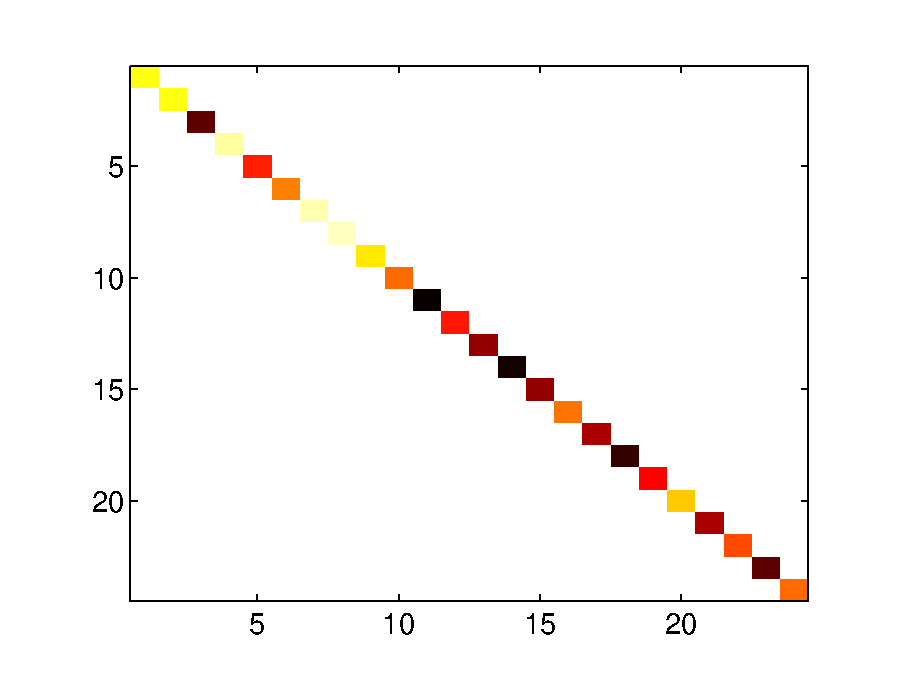
\includegraphics[trim=1.3cm 0 1cm
0.5cm, clip, width=0.45\columnwidth]{figures/covariance_path.eps} }
\subfigure[hidden state of a pose gesture.]{
\includegraphics[trim=1.3cm 0
1cm 0.5cm, clip, width=0.45\columnwidth]{figures/covariance_pose.eps} }
\caption{Visualization of normalized covariance matrices of MoG for different
hidden states. The darker the color, the larger the variance.}
\label{fig:covariance}
\end{figure}

It is possible that a gesture with a distinct path also has the same hand pose
as another gesture with distinct hand pose, for instance, some user may prefer
to do the Circle gesture with a point hand pose. In this case, the gesture
will be recognized as the Circle gesture because it matches both the hand
pose and the path and thus the Circle gesture would have a higher likelihood
after considering a few consecutive frames.

Since there is only one hidden state for $s_{\text{pose}}$, its transition
probability is 1. Its termination probability is estimated according to the
expected duration of the gesture. The self-arc on a state in an HMM defines a 
geometric distribution over waiting time \cite{murphy02}. In the case of a
single state HMM, the probability of remaining in state $s_{\text{pose}}$ for
exactly $d$ steps is $P(d) = p(1-p)^{d - 1}$, where $p = P(END|s_\text{pose})$
is the termination probability for $s_{\text{pose}}$. This means the expected
number of steps remaining in state $s_{\text{pose}}$ is $\frac{1}{p}$. I assume
that the minimum duration of a path gesture is one
second (30 frames). The termination probability $P(END|s_\text{pose})$ is then set to
be less than $\frac{1}{30}$.

I also use one hidden state to model the rest position in a similar way.

\section{Real-time Gesture Recognition}
I train one HMM, $\underline{\theta}_g$, for each gesture (path or pose) $g\in
\{1\ldots G\}$, then combine them into a one-level flattened HMM, assuming uniform transition probabilities among gestures.

\subsection{Combined HMM}
I use the superscript $c$ to denote the model
parameters in the combined HMM. Let $K_{g}$ be the number of hidden states for
gesture $g$. The total number of hidden states in the combined HMM, $K^c$, is then
\begin{align*}
K^c = \sum_g K_{g}
\end{align*}
The model for each path gesture starts with a hidden state for the pre-stroke,
then 1 or 2 hidden states for the nucleus, followed by a hidden state for the
post-stroke. Each pose gesture has a hidden state for the nucleus. The combined HMM has a sequential labeling for these models� hidden states,
with the hidden state label for the pre-stroke of the second gesture model following
the hidden state label for post-stroke of the previous gesture, etc.
Formally, the new hidden states labels are in $\{1\ldots K^c\}$, and
the hidden states from $(\text{base}_i + 1)$ to $(\text{base}_g + K_{g})$
belongs to gesture $g$ where $base_g$ is the base index
\begin{align*}
\text{base}_g = \sum_{j=1}^{g-1}K_{j}
\end{align*}
Figure~\ref{fig:combined-hmm} gives an example of the labeling scheme in
the combined HMM. This scheme allows me to easily map a hidden state label back
to its corresponding gesture and phase.

\begin{figure}[tbh]
\centering
\includegraphics[width=0.9\columnwidth]{figures/combined_hmm.png}
\caption{Combined HMM. The red lines are examples of new transitions. Not all
possible transitions are shown so that the diagram is not cluttered.}
\label{fig:combined-hmm}
\end{figure}

The non-trivial part in creating the combined HMM is computing the new 
transition probabilities. The initial state probability in the combined
HMM, $t^c(s)$, for $s\in\{1\ldots K^c\}$ is
\begin{align*}
t^c(s) = \frac{t(s)}{\sum_{s'=1}^{K^c} t(s')}
\end{align*}
The probability of an $s$ to $s'$ transition
in the combined model is the sum over all paths from $s$ to
$s'$ for $s, s'\in\{1\ldots K^c\}$~\cite{murphy02}. In our model, 
\begin{align}
t^c(s'|s) = t(s' | s) (1-t(\text{END}|s)) +
t(\text{END}|s)t^c(s')
\label{eq:combined-transition}
\end{align}
where $t(s'|s)$ is the transition probability in the individual gesture HMM if
$s$ and $s'$ are from the same gesture; otherwise it is zero. Note that
$t(s'|s)$ is normalized such that $\sum_{s'}t(s'|s) = 1$ without taking into
account the termination probability $t(\text{END}|s)$ (as the end state is not
an actual hidden state), hence it is necessary to multiply $t(s'|s)$ by $
(1-t(\text{END}|s))$ in Equation~\ref{eq:combined-transition} to get the actual
unnormalized probability.

As the pre-strokes and post-strokes for different gestures can be similar, I
allow sharing of the pre-strokes and post-strokes by adding a small probability
(0.01) among pre-stroke hidden states and among post-stroke hidden states.

Finally, we need to make sure that the new transition matrix is stochastic,
i.e., 
\begin{align*}
\sum_{s' = 1}^{K^c} t^c(s'|s) = 1
\end{align*}
by normalizing $t^c(s'|s)$.

\subsection{Online Inference}
Once we have a combined model, I use fixed-lag smoothing \cite{murphy02} to do
online inference on the flattened HMM for real-time gesture recognition.
Fixed-lag smoothing is a modified forward-backward algorithm. Unlike online
filtering, which estimates the belief state at current time $t$ using forward
pass only, we estimate the state at $t - l$, given all the evidence up to the
current time $t$, i.e., compute $\gamma_{t - l}(s) \eqdef P(S_{t -
l} = s|\underline{x}_{1:t})$, where $l > 0$ is the lag. Introducing lag time is
a tradeoff between accuracy and responsiveness. Using some future evidence to
smooth the estimate can increase the accuracy while adding some delay. However
if the delay is small, it might be unnoticeable.
In the Experiment Evaluation section (Section~\ref{sec:evaluation}), we show
details about the relationship between $L$ and the recognition performance.

Fixed-lag smoothing can be implemented efficiently. We compute forward
probabilities $\alpha_t(s) \eqdef P(S_t = s|\underline{x}_{1:t})$
normally\footnote{It is more common (see e.g.,~\cite{Rabiner90}) to define
$\alpha_t(s) = P(S_t = s, \underline{x}_{1:t})$; the difference is discussed in
Section~\ref{sec:hmm-infernece}.} and keep a history window of
$\alpha_{t - l}\ldots\alpha_t$.
At every time frame, we compute backward probabilities $\beta_{t-l}(s)\eqdef
P(\underline{x}_{t-l+1:t}|S_{t-l}=s)$ from current time $t$ to $t - l$, i.e.,
form $l=0$ to $l$.
Then we can compute
\begin{align}
\gamma_{t - l} = \alpha_{t - l} \cdot \beta_{t - l}
\end{align}  
The time complexity at each time frame is $O((K^c)^2l)$. Note that at time $t$,
the belief state at $t - l$ is committed, while the belief state from $t - l + 1$ to $t$
will still be revised later.

We can then compute the most likely hidden state at $t - l$:
\begin{align}
\hat{s} = \arg\max_s \gamma_{t - l}(s)
\end{align}
We map the most likely hidden state to the gesture label it
belongs to (including the rest position) and the gesture phase. 

Gesture events are detected at the boundary of a phase change: start pre-stroke,
start gesture nucleus and start post-stroke. In this way
we achieve simultaneous segmentation and recognition. The gesture event
information, together with the gesture label for the nucleus phase, are sent to the application level.

\begin{figure}[t]
\centering
\includegraphics[trim=0 5mm 0
5mm, clip, width=\columnwidth]{figures/hidden_labeled.jpg}
\caption{Most likely hidden states using fixed-lag smoothing. Different colors indicate different hidden states. Yellow indicates rest position.}
\label{fig:visual_hidden}
\end{figure}

Figure~\ref{fig:visual_hidden} shows a visualization of the
most likely hidden states based on online fixed-lag smoothing inference
with $l = 5$ on a test sequence from the YANG dataset.
This is based on an input sequence of 6 gestures. The first 3 gestures are
Circle and the last 3 gestures are Horizontal Wave gestures. Notice that in
the first segment, at the beginning, the most likely hidden state is the
pre-stroke for Horizontal Wave, but since a response is not required at this
time, the wrong estimate does not matter. After a few more frames, the estimates are
updated to have the correct most likely gesture label and the system
responds correctly when it detects the start of the post-stroke of Circle
gesture.

\section{Gesture Spotting}
Identifying gesture phases allows us to distinguish gestures from non-gestures.
As every gesture must have a nucleus, any hand movement that does not have a
nucleus phase can be identified as non-gesture. 

For example, when performing offline recognition on the ChAirGest dataset, I use
MoG models for rest and non-rest positions to find non-rest segments (i.e.,
segments with hand movement) in a test sequence, and for a non-rest segment, use
the Viterbi algorithm to find the most probable hidden state sequence $\hat{s}_1\ldots\hat{s}_T$ using
the mostly likely gesture model $\underline{\theta}_{\hat{g}}$
(see~\cite{yin13} for details).
Again, each hidden state can by classified into a pre-stroke
($s_\text{pre-stroke}$), nucleus ($s_\text{nucleus}$), or post-stroke
($s_\text{post-stroke}$) state.
The start and the end time for a gesture nucleus are the first and the last time
frame $t$ where $\hat{s}_t\in s_{\text{nucleus}}$ respectively. 

\begin{figure}[tbh]
\centering
\subfigure[Gesture label result.
The pre-stroke and post-stroke phases are indicated by two orange colors (see the color bar).]{
\includegraphics[trim={4cm 1cm 0cm 0.6cm}, clip,
width=1\columnwidth]{figures/gesture.eps}\label{fig:gesture-label}
}
\subfigure[Most probable hidden states.
Colors 1-3 indicate the pre-stroke hidden states, colors 4 - 9
indicate the nucleus hidden states, colors 10 - 12 indicate the post-stroke
hidden states, and color 14 indicates the rest state.]{
\includegraphics[trim={2.5cm 0cm 0.2cm 0cm}, clip,
width=1\columnwidth]{figures/hiddenstates_labeled.jpg} \label{fig:hiddenstates}
}
\caption{Visualization of gesture recognition result. A non-rest segment
without a nucleus phase (see $t\sim 30700$ in \subref{fig:hiddenstates}) is not
identified as a gesture (no label reported at the same time in
\subref{fig:gesture-label}.}
\end{figure}

Figure~\ref{fig:gesture-label} shows the recognition result visualization for
one test sequence. The first row is the ground truth with different colors
indicating different gesture phases or the rest position.
The second row is my segmentation and recognition result.
Figure~\ref{fig:hiddenstates} shows the color-coded most probable hidden states
for the same sequence.
If a non-rest segment does not contain hidden states belonging to the nucleus
phase, it is ignored (see the blue bar at $t\sim 30700$ in Figure~\ref{fig:hiddenstates}).
In this way, we can spot the actual gestures while filtering out other movements.

Using a thresholding method on the loglikelihood of a
given segment may not be robust because the maximum loglikelihood of a non-gesture
segment among all gesture HMMs can be greater than that of a gesture segment.
The HMM formulation (Equation~\ref{eq:hmm}) implies that the longer the sequence the smaller the
likelihood (and hence the loglikelihood) because there are more probability
terms which are all smaller than 1 in the product terms. For example, the
loglikelihood of the fifth non-rest segment (a non-gesture) in
Figure~\ref{fig:hiddenstates} has a maximum loglikelihood of -296.6, while the
first non-rest segment (a gesture) has a maximum loglikelihood of -785.6. 
Even if we normalize the loglikelihoods by the segment lengths, the normalized
loglikelihood for the non-gesture (-14.8) is still greater than that of the
gesture (-17.9). As non-gestures are often shorter than gesture sequences, it
would hard to set a good threshold.
 
My gesture phase based method can be used in addition to a thresholding method
with a relative conservative threshold, i.e., a threshold that may cause false
positives but no false negatives so that the gesture phase based method can be used to further
filter out false positives.

\section{Concatenated HMM versus LDCRF}
LDCRF gives per frame classification in an unsegmented sequence. Where
there are ground truth labels for gesture phases (e.g., the ChAirGest
dataset), we can also use LDCRF to do embedded training of the gesture
phases. For a given non-rest segment, 

different hidden states for different pre-stroke and post-stroke phases
for different gestures, increases computation time significantly since it increases quadratically with number of hidden states.
Constrain transition

Compare temporal data modeling: HMM and CRF. 
\chapter{Online Recognition Evaluation}\label{sec:evaluation}
The previous sections reported evaluation results most pertinent
to the sections under discussion. This chapter presents results
for the overall online recognition performance.

\section{Evaluation Protocol}
I evaluate the online gesture recognition performance using the YANG
dataset and the hybrid performance
metrics proposed in Section~\ref{sec:metrics}. The evaluation is based on the
assumption that all the path gestures are
discrete flow gestures, and pose gestures are continuous flow
gestures.
The survey results shown earlier in Section~\ref{sec:preferences} show that it
is important to allow users to quickly define and train their own gestures. Hence,
I evaluate my system using user dependent training and testing. For each user
in the dataset, I use the first 2 sessions of recording (6 samples per gesture)
as training examples, and the last 2 sessions as testing examples. The first 2
sessions have ``Rest'' prompts which help to do automatic segmentation on the
training data. All the results reported are the average test results from 10
users.

Figure~\ref{fig:recog-result} shows a visualization of the recognition result on
a test sequence. The figure highlights the challenges in the test sequences:
there are 21 gestures in each continuous unsegmented sequence; 
gestures sometimes follow one another immediately.

\begin{figure}[thb]
\centering
\includegraphics[trim=43mm 15mm 42mm 10mm, clip,
width=\columnwidth]{figures/recog_result.png}
\caption{Comparison between recognition result using online inference
and ground truth.
The colors correspond to different gestures. For discrete flow gestures
(Swipe Left/Right, Circle, Horizontal Wave), one color segment with a fixed
length is shown at the time of response. For continuous flow gestures, the
recognized gesture is shown at each frame indicating frame-by-frame responses.}
\label{fig:recog-result}
\end{figure}

\section{Effect of the Number of Principal Components}
PCA reduces the dimensionality of the feature vectors, and hence, reduces the
computational complexity. I use cross-validation to find the
best number of principal components that accounts for the
variation in the data while keeping the dimension at the
minimum. Figure~\ref{fig:pca} shows how the recognition $F_1$ scores depends on
the number of principal components used for the HOG descriptor.
The best average score is obtained with 15 principal components.

\begin{figure}[tbh]
\centering
\includegraphics[width=\columnwidth]{figures/f1_pca.png}
\caption{Graph showing how $F_1$ scores for discrete flow gestures, continuous
flow gestures and the average scores change with the number of principal
components used for the HOG descriptor.}
\label{fig:pca}
\end{figure}

\section{Compare Different Topologies}
In this section, I compare my unified framework with a common HMM-based approach
used in previous works~\cite{sharma00, Starner95}, which use the same
topology for all gestures.

Table~\ref{tab:result} compares the results between the two methods.
The third column is the result from treating the two \textit{forms} of gestures
in the same way, i.e., all gestures have the same left-right Bakis topology for their
nucleus phases. The fourth column is the result from using a left-right Bakis
topology for path gestures and a single state topology for pose gestures. To
ensure a fair comparison, all hidden states have 3 mixtures of Gaussians. As Table~\ref{tab:result}
shows, having different HMM topologies for the two \textit{forms} of gestures
significantly increases the recall and $F_1$ score for pose gestures.

\begin{table}[tbh]
\centering
\begin{tabular}{|l|l|p{3cm}|p{3cm}|}
\hline
& & \textbf{Same topology for two forms of gestures} & \textbf{Different
topologies for two forms of gestures} \\
\hline
\multirow{4}{4cm}{Path \& discrete flow gestures} 
& Precision & \textbf{0.84 (0.16)} & 0.82 (0.16) \\
\cline{2-4}
& Recall & 0.87 (0.17) & 0.87 (0.18)\\
\cline{2-4}
& $F_1$ & \textbf{0.85 (0.16)} &  0.84 (0.16)\\
\cline{2-4}
& Responsiveness (s) & 0.6 (0.3) & 0.6 (0.3) \\
\hline
\multirow{4}{4.5cm}{Pose \& continuous flow gestures}
& Precision & \textbf{0.65 (0.14)} & 0.63 (0.11) \\
\cline{2-4}
& Recall & 0.41 (0.15) & \textbf{0.65 (0.09)} \\
\cline{2-4}
& $F_1$ & 0.50(0.14) & \textbf{0.64 (0.10)} \\
\hline
\textbf{Average} & $F_1$ & 0.675 (0.150) & \textbf{0.740 (0.130)} \\
\hline
\end{tabular}
\caption{Results from using different topologies. The numbers in parentheses are
standard deviations. The results are based on using 3 mixtures of Gaussians
for all hidden states, and lag time
$l = 8$ frames.}
\label{tab:result}
\end{table}

For gestures with arbitrary movement (e.g., pose gestures), it is difficult to
use embedded training to accurately align pre-stroke, nucleus and post-stroke
phases, because training sequences can have very different lengths, and so do
the testing sequences.
Figure~\ref{fig:palm-hidden} shows the estimates of
the most likely hidden states for a Palm Up gesture sequence when the same
left-right topology are used for both \textit{forms} of gestures is used.
The main (center) part of the gesture, which should be the nucleus of the gesture, is identified
as the post-stroke. This is why it is important to have different topologies and
different training strategies for the two forms of gestures.

\begin{figure}[tbh]
\centering
\includegraphics[width=0.3\linewidth]{figures/palm_hidden_label.png}
\caption{Estimated hidden states for a Palm Up gesture using the
left-right model the same as path gestures. Different colors correspond to
different hidden states.}
\label{fig:palm-hidden}
\end{figure}

\section{Effect of Different Numbers of Mixtures}
The previous section shows that using different topologies for path and pose
gestures give better
recognition performance. So using this model, I investigate the effects
of the number of mixtures ($k$) in the MoG emission probabilities.

First, I set $k$ be the same for both forms of gestures.
Fig.~\ref{fig:mixtures} shows that the $F_1$ score increases as the number of
mixtures increases until $k=3$.
After that, we start to see the effect of overfitting.

\begin{figure}[tbh]
\centering
\includegraphics[trim=10mm 5mm 10mm 15mm,
clip, width=\columnwidth]{figures/f1_nM.png}
\caption{F1 scores versus number of mixtures.}
\label{fig:mixtures}
\end{figure}

I then experimented with using different $k$'s for path and pose gestures. For
path gestures, I
set $k^\text{path} = 3$, and use a different number of
mixtures, $k^{\text{pose}}_g\in \{3\ldots6\}$, for each pose gesture $g$. Each
$k^{\text{pose}}_g$ is chosen according to the Bayesian Information Criterion
(see Section~\ref{sec:pose-gesture}).
Using this method, I am able to improve precision, recall and $F_1$ scores for
both forms of the gestures even further (see
Table~\ref{tab:different-mixtures}).

\begin{table}[tbh]
\centering
\begin{tabular}{|p{4.5cm}|l|p{4cm}|}
\hline
& & \textbf{Use different topologies and numbers of mixtures} \\
\hline
\multirow{4}{4cm}{Path \& discrete flow gestures} 
& Precision & \textbf{0.94 (0.05)} \\
\cline{2-3}
& Recall    & \textbf{0.93 (0.08)} \\
\cline{2-3}
& $F_1$ & \textbf{0.93 (0.06)} \\
\cline{2-3}
& Responsiveness (s) & 0.6 (0.2)  \\
\hline
\multirow{3}{4cm}{Pose \& continuous flow gestures}
& Precision & \textbf{0.68 (0.10)} \\
\cline{2-3}
& Recall & \textbf{0.69 (0.08)} \\
\cline{2-3}
& $F_1$ & \textbf{0.68 (0.09)}  \\
\hline
\textbf{Average} & $F_1$ & \textbf{0.805 (0.075)}\\
\hline
\end{tabular}
\caption{Results from using different numbers of mixtures of Gaussians
for the emission probabilities ($l = 8$ frames).}
\label{tab:different-mixtures}
\end{table}

%Compare user dependent vs user independent result

\section{Effect of Different Lag Times}
Figure~\ref{fig:lag} shows how the $F_1$ scores change with respect to the lag
time ($l$) in fixed-lag smoothing. The performance increases as $l$ increases, and
plateaus at $l=8$ frames which is about 0.3s at 30 FPS. This shows that more
evidence does help to improve the estimates until a limit, and we do not need to
sacrifice too much delay to reach the limit. Our result also shows that the
responsiveness score (RS, defined in Equation~\ref{eqn:rs}) stays around 0.6--0.7
seconds as $l$ is increased.

\begin{figure}[!tbh]
\centering
\includegraphics[trim=0 5mm 0 15mm, clip,
width=\columnwidth]{figures/f1_lag.png}
\caption{$F_1$ score versus lag time $l$.}
\label{fig:lag}
\end{figure}

\section{Training Time}
The HMM-based unified framework is fast to train. The average
computation time for training the model for one user is about 5s with 7 gestures and 6 training examples per
gesture. 

Because of the fast training process, the system is easily extensible. New
gestures can be added by recording 3-6 repetitions of the gesture using the Kinect; the system will train an HMM model for the gesture
and add it to the existing combined HMM. This process, including the recording
time, takes only a few minutes.

\section{User Independent Evaluation}
Our survey (Section~\ref{sec:preferences}) indicated that users
generally prefer a system to have a predefined gesture set and then add or
change gestures later according to their own preferences. This means that having
a user independent base model will be useful as well. If the system has user
provided training examples for certain gestures, it uses the
user dependent models for those gestures; otherwise it backs off to the base
model. This adaptation strategy is similar to~\cite{yin13-making}.

To evaluate the user independent model, I did a 10-fold cross-validation where
in each fold, the data from one user's last 2 sessions are used for testing and
the data from the remaining 9 users' first 2 sessions are used for training.
Table~\ref{tab:user-independent} shows the average, best and worst results among
the users. We can see that there is large variation among the users. Users
who want to do the gestures differently need to train their user
dependent models. For example, the results based on user dependent model for user PID-02
is much better than the user independent model.

\begin{table}[tbh]
\centering
\begin{tabular}{|p{3cm}|l|l|p{1.9cm}|p{1.9cm}||p{2cm}|}
\hline
& & \textbf{Average} & \textbf{Best (PID-01)} & \textbf{Worst (PID-02)} &
\textbf{User dep. (PID-02)} \\
\hline
\multirow{4}{3cm}{Path \& discrete flow gestures} 
& Precision & 0.72 (0.18) & 1.00 & 0.35 & 0.96 \\
\cline{2-6}
& Recall    & 0.72 (0.16) & 1.00 & 0.72 & 1.00\\
\cline{2-6}
& $F_1$ & 0.70 (0.16) & 1.00 & 0.47 & 0.98 \\
\cline{2-6}
& Responsiveness (s) & 0.6 (0.3)  & 0.6 & 0.4 &  0.4\\
\hline
\multirow{3}{3cm}{Pose \& continuous flow gestures}
& Precision & 0.59 (0.12) & 0.79 & 0.49 & 0.67\\
\cline{2-6}
& Recall & 0.56 (0.16) & 0.77 & 0.21 & 0.67\\
\cline{2-6}
& $F_1$ & 0.56 (0.13)  & 0.78 & 0.29 & 0.67\\
\hline
\textbf{Average} & $F_1$ & 0.63 (0.15) & 0.89 & 0.38 & 0.83\\
\hline
\end{tabular}
\caption{User independent model 10-fold cross validation results ($l = 8$
frames). The last column is the user dependent result for user PID-02 for
comparison.}
\label{tab:user-independent}
\end{table}

\section{Discussion}
Our overall best performance for the YANG dataset is reported in
Table~\ref{tab:different-mixtures}. The performance for the pose and
continuous flow gestures is relatively low compared to that of the path and
discrete flow gestures. Most
confusions are among the 3 pose gestures, i.e., Point, Palm Up, Grab (see
Figure~\ref{fig:recog-result} for example).
There are big variations in the recognition results for the pose gestures among users: the highest $F_1$ score for pose gestures is 0.81
and the lowest is 0.58. For the ones with low $F_1$ scores, confusion occurs
when there is significant motion blur (see Figure~\ref{fig:point_grab}). These
correspond to the users who move relatively fast when doing the pose gestures.
This suggests that with the frame rate of the Kinect sensor used (30Hz for
the Kinect version One), users may need to perform pose gestures relatively
slowly in order to get better recognition results, or a better (higher rate)
sensor is needed.

\begin{figure}[tbh]
\centering
\includegraphics[width=\linewidth]{figures/point_posture_full_image.png}
\caption{This frame is mistakenly classified as Grab while the true gesture
is Point. Motion blur is significant.}
\label{fig:point_grab}
\end{figure}
\begin{savequote}[120mm]
Each gesture is created at the moment of speaking and highlights what is
relevant and the same entity can be referred to by gestures that have changed
their form.
\qauthor{David McNeill, \textit{Hand and mind: what gestures reveal about
thought}}
\end{savequote}
\chapter{Gesture Interaction}
\section{Continuous and Discrete Gestures}
How to handle continuous and discrete gestures in an unified probabilistic
framework. Use hand poses to distinguish continuous and discrete gestures.
Unlike \cite{Oka02} et al., hand poses are selected based on naturalness.

\section{Gesture and Speech}
Traditionally, gestures are used to augment speech in interaction, as pioneered
by Bolt's ``Put That There'' system \cite{Bolt80}. Our previous user study
\cite{yin10thesis} show that speech also can augment gestures.

We use an off-the-shelf speech 
recognizer, and investigate how to combine both speech and gesture to make
the interaction more natural and effortless. Specifically, we will explore how speech and gestures complement each other in certain scenarios.

Two types of events: gesture and speech.

\begin{lstlisting}[caption=Gesture event JSON object]
{"gesture": <gestureName>, 
 "type": <"StartPreStroke" | "StartGesture" | "StartPostStroke">,
 "stage": <"PreStroke" | "Gesture" | "PostStroke">,
 "rightX": <rightHandXWorldCoordinate>,
 "rightY": <rightHandYWorldCoordinate> } 
\end{lstlisting}

\begin{lstlisting}[caption=Speech event JSON object]
{"speech": <speechTag>}
\end{lstlisting}

Number of hidden states for gestures with dynamic paths should at lest be 3.

\section{Gesture Controlled Presentation}
Server client architecture

Multimodal input server sends recognized gesture and speech events over a
WebSocket\footnote{http://en.wikipedia.org/wiki/WebSocket}. Any client
application can subscribe to the input events by connecting to the server
socket. The events are serialized in JSON format\footnote{http://www.json.org/}. 

\begin{savequote}
Language is a part of social behavior. What is the mechanism whereby the social
process goes on? It is the mechanism of gesture\ldots
\qauthor{George Herbert Mead, \textit{Mind, self, and society}}
\end{savequote}
\chapter{Conclusion}
I developed a real-time continuous gesture recognition system for natural
human computer interaction. The
unified probabilistic framework for handling two forms of gestures is a novel
approach, and the evaluation shows promising results: an
average online recognition $F_1$ score of 0.805 using the hybrid performance
metric, on a challenging dataset with unsegmented gestures of different forms.
The system also achieves real-time performance at 30FPS. Using the framework, I
developed a gesture controlled presentation application similar to the one described at the beginning of this paper. All the code is open-source
and is available
online\footnote{\url{http://groups.csail.mit.edu/mug/projects/gesture_kinect/index.html\#code}}.

Another novel approach is using embedded training and hidden state information
to detect gesture phases, allowing the system to respond more promptly. On
average, for discrete flow gestures, the system responds 0.6s before the hand comes to
rest. 

I collected a new dataset that includes two forms of gestures, a
combination currently lacking in the community, and plan to make it
public. I also proposed a hybrid performance metric
that is more relevant to real-time interaction and different types of gestures.

\section{Limitations}
Currently, the system only handles single-hand gestures, it will not be hard to
add two-hand gestures. The only difference will be the feature vector which
should be a concatenation of features from both hands. The recognition module
would remain the same.

The number of hidden states per gesture needs to be specified by the user or the
application developer in the gesture definition file. In the future work, we
will make the system automatically learn the number of hidden states through
cross-validation and by grouping similar frames~\cite{song13}.

The performance for pose gestures is lower than that
for path gestures. Two factors contribute to this problem: the limitation in
both the pixel and the depth resolutions of the Kinect sensor, and motion blur.
It would be interesting to test with the new version of the Kinect sensor which
uses a time-of-flight depth sensor and is reported to have a higher resolution. Other feature descriptors
(e.g., histograms of optic flows) and encoding methods (e.g, sparse
coding~\cite{lee07}) can be explored as well.

The performance of a user independent model is relatively low. This is expected
because there is large variation among users. Even though, users can
quickly define and train their own models, an relatively accurate base
model is always valuable. Hence, more work can be done to improve the base
model, e.g., using mixture of HMMs~\cite{keskin12}.

\section{Future Work}
In addition to work that address the limitations. There is future research to
consider to push the frontier of natural human computer interaction further.

\textbf{Sensors} In this thesis, I considered the Kinect and the IMU as
input sensors. The gesture controlled presentation application currently
only uses the Kinect data. We can explore even more combinations of sensors
by including the Leap Motion Controller and smartwatches. Each sensor has
strengths of their own, so by combining them we can get the best system
overall. The Leap Motion Controller is mostly used as an environmental sensor,
but we can also explore its use case a wearable sensor. Its high accuracy in
finger tracking may help improve recognition performance for pose gestures.

\textbf{User adaptation} This is a hot topic in both machine learning and
HCI, and is applicable to many domains such as speech recognition and
touch screen keyboard input~\cite{yin13-making}. Currently, the system
uses a binary decision to do user adaptation: if a user-trained model is
present, the system will use that model; otherwise it uses the base
model. It would be more convenient if the system learns the user
dependent model implicitly when the user is using the system, and uses
soft decision to combine the base model and user dependent model, e.g., weighted
combination.

\textbf{Interactive training} Due to large variation in users performing
gestures and difference in user preference, the gesture recognition system would
benefit from having an easy to use interface for fast training. Many machine
learning related research assumes the availability of training data. Creating
interfaces that are easy for users to provide training examples, either in a
separate session, or when using the system and provide feedback to the system
for wrong recognition would be an interest interdisciplinary topic in machine
learning and HCI.

\appendix
\chapter{Review of F-measure}\label{app:fmeasure}
In statistical analysis of binary classification, the F-measure is a measure of
test's accuracy, combining both the precision and the recall of the test.
Precision is the fraction of correct results from all the returned results
(i.e., the number of correct results divided by the number of all returned
results), and recall is the fraction of correct results from all the results
that should be returned (i.e., the number of correct results divided by the
number of results that should have been returned)~\cite{f1score14}. Note that
both precision and recall have the same numerator.

The general formula for F-measure is
\begin{align*}
F_\beta &= (1 + \beta^2)\cdot\frac{\text{precision}\cdot
\text{recall}}{(\beta^2\cdot\text{precision}) + \text{recall}}\\
&= \frac{1 + \beta^2}{\frac{1}{\text{precision}}+\frac{\beta^2}{\text{recall}}}
\end{align*}
which is the weighted harmonic mean of precision and recall. The $F_1$ score
($\beta=1$) is the most commonly used one where precision and recall have
equal weight:
\begin{align*}
F_1 = 2\cdot\frac{\text{precision}\cdot
\text{recall}}{\text{precision} + \text{recall}}
\end{align*}
Two other commonly used F measures are the $F_2$ measure, which weighs recall
higher than precision, and the $F_{0.5}$ measure, which puts more emphasis on
precision than recall.


%\chapter{Review of Kalman Filter}\label{app:kalman}
This chapter is based on the OpenCV book~\cite{Opencv}. The Kalman filter is an
algorithm that uses a series of measurements observed over time, containing
noise and other inaccuracies, and produces estimates of unknown variables that
tend to be more precise than those based on a single measurement
alone~\cite{kalman14}.
Let $\underline{x}_t$ be an $d$-dimensional vector of state components of a
system.
Assuming no external control, the a priori estimate $
\underline{x}_t^-$ of the state is
given by:
\begin{align*}
\underline{x}_t^- = F\underline{x}_{t - 1} + \underline{w}_t,
\end{align*}
where $F$ is the $d$-by-$d$ \textit{transfer matrix} characterizing the
dynamics of the system, and $\underline{w}_t$ is the \textit{process noise}
associated with random events or forces that directly affect the actual state of
the system. We assume that the components of $\underline{w}_k$ have Gaussian
distribution $N(\underline{0}, Q_t)$ for some $d$-by-$d$ covariance matrix $Q_t$.

Using $P_t^-$ to denote the error covariance, the a priori estimate for this
covariance at time $t$ is obtained from the value at time $t - 1$ by:
\begin{align*}
P_t^- = FP_{t - 1}F^T + Q_{t - 1}
\end{align*}

In general, we make measurement $\underline{z}_t$ that may or may not be the
direct measurements of the state variable $\underline{x}_t$. The measurement
$\underline{z}_t$ is an $m$-dimensional vector given by:
\begin{align*}
\underline{z}_t = H_t\underline{x}_t + \underline{v}_t,
\end{align*}
where $H_t$ is an $m$-by-$d$ matrix and $\underline{v}_k$ is the measurement
error.

The \textit{Kalman gain}, $K_t$, is an $d$-by-$m$ matrix,  
\begin{align*}
K_t = P_t^-H_t^T(H_tP_t^-H_t^T + R_t)^{-1}
\end{align*}
It tells us how to
weight new information against what we think we already know.
The updated value for $\underline{x}_k$ when a new measurement is available is:
\begin{align*}
\underline{x}_t = \underline{x}_t^- + K_t(\underline{z}_t^- -
H_t\underline{x}_t^-)
\end{align*}
The update value for $P_t$ is:
\begin{align*}
P_t = (I - K_tH_t)P_t^-
\end{align*}



\chapter{Principal Component Analysis Optimizations}\label{app:pca}
Principal Component Analysis (PCA) computes a new basis to re-express the
dataset.
The new basis is a linear combination of the original basis, and all the new basis vectors are orthonormal
and are in the directions of largest variations~\cite{shlens2005}. This appendix
explains some optimizations I did to speed up PCA computation.

\section{No Scaling}

Assume we have $n$ data points and each data point is represented by a feature
vector with dimension $d$. Let matrix $X$ be the ``centered'' data (i.e., every
feature has mean 0), where columns are data points and rows are features (i.e,
a $d\times n$ matrix), then $n\Sigma = XX^T$, where $\Sigma$ is the covariance
matrix of the data and $n$ is the number of data points. The principal components of the data are the eigenvectors of
$\Sigma$.

Since $XX^T$ and $\Sigma$ are real symmetric matrices, their eigenvectors can be
chosen such that they are real, orthogonal to each other and have norm one. Let
$Q_X\Lambda_X Q_X^T$ be the  eigendecomposition of $XX^T$ and $Q\Lambda Q^T$ be
the eigendecomposition of $\Sigma$, and $Q_X$ and $Q$ have unit column
vectors, then we have
\begin{align*}
nQ\Lambda Q^T &= Q_X\Lambda_X Q_X^T  \\
\Lambda &= \frac{1}{n}\Lambda_X \\
Q &= Q_X
\end{align*}

This shows that PCA is invariant to the scaling of the data, and will return the
same eigenvectors regardless of the scaling of the input~\cite{pca14}. Only the
eigenvalues will be scaled by the same factor if the input is scaled. 

The total variance in the data is defined as the sum of the variances
of the individual components, i.e., the sum of eigenvalues of $\Sigma$. Let
$\lambda_1, \lambda_2, \ldots, \lambda_n$ be the eigenvalues of $\Sigma$
(sorted in descending order), i.e., the diagonal entries of $\Lambda$. Variation
explained by $k$ principal components is then given by
\begin{align}
\frac{\sum_{i=1}^{k} \lambda_i}{\sum_{i=1}^{n}\lambda_i}
\end{align}
We can use the diagonal entries from $\Lambda_X$ to compute the variation
explained because the scaling factor will be canceled out.

\section{Transpose $X$}
If $d$ is much larger than $n$, it is more
efficient\footnote{\url{http://onionesquereality.wordpress.com/2009/02/11/face-recognition-using-eigenfaces-and-distance-classifiers-a-tutorial/}}
to compute $X^TX$ which is a $n\times n$ matrix instead of $d\times d$. If we find the eigenvectors of this matrix, it would return $n$ eigenvectors, each of dimension $n$.

Let $Q_{X^T}\Lambda_{X^T}Q_{X^T}^T$ be the eigendecomposition of $X^TX$. Let
$v_i$ be an eigenvector of $X^TX$ (i.e., $v_i$ is a column vector of $Q_{X^T}$),
and $u_i$ be an eigenvector of $XX^T$ (i.e., $u_i$ is a column vector of
$Q_{X}$). We can show that
\begin{align*}
(XX^T)^2  = XQ_{X^T}\Lambda_{X^T}Q_{X^T}^TX^T = Q_X\Lambda_X^2 Q_X^T
\end{align*}
This means that $u_i = s_iXv_i$ where $s_i$ is a scaling factor that normalizes
$Xv_i$. Let $\lambda_i^v$ and $\lambda_i^u$ be the eigenlavues corresponding to
$v_i$ and $u_i$.
\begin{align*}
X^TXv_i &= \lambda_i^v v_i \\
XX^TXv_i &= \lambda_i^v Xv_i \\
XX^Tu_i &= \lambda_i^v u_i = \lambda_i^u u_i\\
\end{align*}
This proves that $\lambda_i^u = \lambda_i^v$.

The above shows that we can obtain $u_i$ and $\lambda_i^u$ from $v_i$ and
$\lambda_i^v$.

\chapter{Review of Dynamic Bayesian Network}\label{app:dbn}
This part is mainly based on the Ph.D. thesis by Murphy \cite{murphy02}.

A dynamic Bayesian network (DBN)~\cite{dean89} is a way to extend Bayes nets to
model probability distribution over semi-infinite collection  of random variables. An
HMM is a stochastic finite automaton, where each state generates (emits) an observation. If we let $S_t$ represent the hidden state at time $t$, the
transition model between states can be characterized by a conditional
multinomial distribution: $A(i, j) = P(S_t = j | S_{t-1} = i)$, where $A$ is a
stochastic matrix.

\section{Inference}
Normalize $\alpha$, so that $\alpha_t(i) = P(X_t = i | y_{1:t})$ which always
sums to one over $X_t$. Sum of $\beta_t = P(y_{t+1:T}|X_t)$ over $X_t$ need not
be one.

\section{Filtering}
The most common inference problem in online analysis is to recursively estimate
the belief state using Bayes's rule:

\begin{align*}
P(S_t | x_{1:t}) & \propto P(x_t | S_t, x_{1:t-1})P(S_t | x_{1:t-1}) \\
         & = P(x_t | S_t) \left[\sum_{s_{t - 1}}
           P(S_t | s_{t - 1})P(s_{t - 1} | x_{1:t - 1})\right]
\end{align*}

This task is traditionally called ``filtering'', because we are filtering out
the noise from the observations. We can find this value using the forward
algorithm.

\section{Classification}
The likelihood of a model, $M$, is $P(x_{1:t}|M)$. This can be used to classify
a sequence as follows:
\begin{align*}
C^*(x_{1:T}) = \arg \max_{C} P(x_{1:T} | C)P(C)
\end{align*}
\chapter{Hidden Markov Models}\label{app:hmm}
An HMM is an example of a state-space model. It is a stochastic
finite automaton, where each state generates (emits) an
observation~\cite{murphy02}. 

\section{Inference}\label{sec:hmm-infernece}
The main inference algorithm for HMMs is the forward-backward algorithm. We
compute $\alpha$ recursively in the forward pass as follows:
\begin{align*}
\alpha_t(s) &= P(S_t=s|\underline{x}_{1:t}) \\
            &= \frac{P(\underline{x}_{1:t-1})P(S_t=s,
            \underline{x}_{1:t})}{P(\underline{x}_{1:t})P(\underline{x}_{1:t-1})}\\
            &= \frac{1}{c_t}P(S_t=s,
\underline{x}_t|\underline{x}_{1:t-1})
\end{align*}
where
\begin{align*}
P(S_t=s,\underline{x}_t|\underline{x}_{1:t-1}) &=
\frac{P(S_t=s,\underline{x}_{1:t})}{P(\underline{x}_{1:t-1})} \\
&=
\frac{P(S_t=s,\underline{x}_{1:t-1})P(S_t=s,\underline{x}_{1:t})}{P(\underline{x}_{1:t-1})P(S_t=s,\underline{x}_{1:t-1})}\\
&= P(S_t=s|\underline{x}_{1:t-1})P(\underline{x}_t|S_t=s) \quad \text{(Markov
property)}\\
&= \sum_{s'}P(S_t=s, S_{t-1}=s'|\underline{x}_{1:t-1})P(\underline{x}_t|S_t=s)
\\
&= \left[\sum_{s'}P(S_t=s |
S_{t-1}=s')P(S_{t-1}=s'|\underline{x}_{1:t-1})\right] P(\underline{x}_t|S_t=s)\\
&= \left[\sum_{s'}P(S_t=s |
S_{t-1}=s')\alpha_{t-1}(s')\right] P(\underline{x}_t|S_t=s)
\end{align*}
and
\begin{align*}
c_t=P(\underline{x}_t|\underline{x}_{1:t-1})=\sum_s P(S_t=s,
\underline{x}_t|\underline{x}_{1:t-1})
\end{align*}

Without the normalization term $c_t$, we would be computing
$\alpha_t(s)=P(S_t=s, \underline{x}_{1:t})$ which is the original definition of
the forward probability. Normalization prevents underflow, and also gives a more
meaningful quantity (a filtered state estimate)~\cite{murphy02}. We keep track
of the normalizing constants so that we can compute the likelihood of the
sequence:
\begin{align*}
P(\underline{x}_{1:T}) =
P(\underline{x}_1)P(\underline{x}_2|\underline{x}_1)P(\underline{x}_3|\underline{x}_{1:2})\ldots
P(\underline{x}_T|\underline{x}_{1:T-1})    = \prod_{t=1}^T c_t
\end{align*}

In the backward pass, we compute $\beta_t(i)\eqdef
P(\underline{x}_{t+1:T}|S_t=i)$, the sum of probabilities of all paths starting
with state $s$ at position $t$ and going to the end of the sequence. Combining
forward and backward passes produces the final answer 
\begin{align*}
\gamma_t(i)\eqdef
P(S_t=i|\underline{x}_{1:T})\propto \alpha_t(s)\beta_t(s)
\end{align*}

\section{Termination Probability}\label{sec:term}
Suppose $s\in \{1, 2, \ldots, K\}$, we add an special state END, so 
$s\in \{1, 2, \ldots, k, END \}$. We also add a special observation at the end
of the sequence $x_{1:T}$ to get $(x_{1:T}, x_{END})$. 
The model takes the following form:
\begin{align*}
P(x_{1:T}, x_{END}, s_{1:T}, END;\underline{\theta}) = 
    t(s_1)t(END|s_T)\prod_{t = 2}^T t(s_t | s_{t-1})\prod_{t = 1}^T e(x_t|s_t)
\end{align*} 
We define the following
\begin{align*}
e(x_{END} | END) &= 1 \\
e(x_{END} | s) &= 0 \text{ for } s\neq END \\
e(x_i | END) &= 0 \text{ for } i \neq END \\
t(s | END) &= 0 \quad \forall s \\
\alpha_t(END) &= 
\begin{cases}
\sum_{s'\in\{1\ldots K\}}\hat\alpha_{t-1}(s')\times t(END|s'), & \text{if } t ==
T + 1
\\
0, & \text{if } t\leq T
\end{cases} \\
\beta_{T + 1}(s) &= 1 \quad \forall s \\
\beta_T(s) &= \beta_{T + 1}(END)\times t(END | s) = t(END | s) \\
\beta_t(END) &= 0 \text{ for } t \leq T
\end{align*}

We want to find $t(END | s)$ for $s\neq END$. The EM update for $t(END|s)$ is
\begin{align*}
t(END|s) &= \frac{\sum_{i = 1}^n \overline{\text{count}}(i, s\rightarrow
END;\underline{\theta}^-)} {\sum_{i = 1}^n\sum_{s'} \overline{
\text{count}}(i, s\rightarrow s';\underline{\theta}^-)} 
\end{align*}
\begin{align*}
\overline{\text{count}}(i, s\rightarrow END;\underline{\theta}) &= P(S_T = s,
S_{T + 1} = END | x_{i, 1:T}, x_{END}; \underline{\theta});\\
    &\propto \alpha_T(s)\times t(END|s)\times \beta_{T +
    1}(END)\\
    &= \alpha_T(s)\times t(END|s)\\
    &= \alpha_T(s)\times \beta_T(s) \propto \gamma_T(s)
\end{align*}
We do not need to compute the constant of proportionality explicitly
because we normalize $\gamma_t(s)$ at each time step.

Finally, the likelihood of the sequence is
\begin{align*}
P(x_{1:T}, x_{END}; \underline{\theta})
    &= \prod_{i = 1}^T c_i \sum_{s\in \{1\ldots K\}}\alpha_T(s)\times
    t(END|s)
\end{align*}

\section{Learning}
\subsection{Baum-Welch Training}
The Baum-Welch algorithm uses the well know Expectation Maximization (EM)
algorithm to find the maximum likelihood estimate of the parameters of a
HMM model given a set of observed feature vectors~\cite{baum-welch14}.

For discrete output, the update for the emission probability at each iteration
is
\begin{equation*}
e(x|s) = \frac{\sum_{i=1}^n \overline{\text{count}}(i, s\leadsto x;
\underline{\theta}^-)}{\sum_{i=1}^n \sum_x \overline{\text{count}}(i,
s\leadsto x;
\underline{\theta}^-)}
\end{equation*}
where $\overline{\text{count}}(i, s\leadsto x;
\underline{\theta})$ is the expected number of times the state $s$ is
paired with paired with the emission $x$ in the training sequence $i$ for
parameters $\underline{\theta}$.

For continuous output with Gaussian emission probability, the updates are 
\begin{align*}
\underline{\mu}_s &= \frac{\sum_{i=1}^n\sum_{t=1}^T P(S_t = s |
\underline{x}_{i, 1:T};\underline{\theta}^-)\underline{x}_{i,
t}}{\sum_{i=1}^n\sum_{t=1}^T P(S_t = s | \underline{x}_{i,
1:T};\underline{\theta}^-)} \\
&= \frac{\sum_{i=1}^n\sum_{t=1}^T \gamma_j(s)\underline{x}_{i,
t}}{\sum_{i=1}^n\sum_{t=1}^T \gamma_t(s)} \\
\Sigma_s &= \frac{\sum_{i=1}^n\sum_{t=1}^T \gamma_t(s)(\underline{x}_{i,
t} - \underline{\mu}_s^-)(\underline{x}_{i, t} -
\underline{\mu}_s^-)^T}{\sum_{i=1}^n\sum_{t=1}^T \gamma_t(s)}
\end{align*}
The $^-$ superscript denotes parameters from the previous iteration.

For continuous output with mixture of Gaussians emission probability, the update
are
\begin{align*}
\underline{\mu}_{s,q} &= \frac{\sum_{i=1}^n\sum_{t=1}^T P(S_t = s, Q_t=q |
\underline{x}_{i, 1:T};\underline{\theta}^-)\underline{x}_{i,
t}}{\sum_{i=1}^n\sum_{t=1}^T P(S_t = s, Q_t=q | \underline{x}_{i,
1:T};\underline{\theta}^-)} \\
\Sigma_{s,q} &= \frac{\sum_{i=1}^n\sum_{t=1}^T p(S_t = s, Q_t=q |
\underline{x}_{i, 1:T};\underline{\theta}^-)(\underline{x}_{i, t} -
\underline{\mu}_s^-)(\underline{x}_{i, t} -
\underline{\mu}_s^-)^T}{\sum_{i=1}^n\sum_{t=1}^T p(S_t = s, Q_t=q |
\underline{x}_{i, 1:T};\underline{\theta}^{t-1})}\\
P(S_t = s, Q_t=q |
\underline{x}_{i, 1:T};\underline{\theta}^-) &=
\gamma_t(s)P(Q_t=q|S_t=s, \underline{x}_{i,t})\\
&=\gamma_t(s)\frac{P(Q_t=q|S_t=s)N(\underline{x}_{i, t};\mu_{s,q},
\Sigma_{s, q})}{e(\underline{x}_{i, t}|s)}
\end{align*}

% \begin{eqnarray}
% Var(X) &= E[(X - \mu)^2]
% \end{eqnarray}
\subsection{Viterbi Training}\label{sec:viterbi}
Instead of summing over all possible paths as in Baum-Welch training, Viterbi
training only considers the single most likely path computed using the Viterbi
algorithm. In each iteration, the Viterbi path for each training sequence is
computed, and the model parameters are updated. For single Gaussian emission
probability, the update at iteration $t$ is
\begin{align*}
t^t(s'|s) &=\frac{\sum_{i=1}^n \text{count}(i, s\rightarrow s';
\underline{\theta}^{t-1})}{\sum_{i=1}^n \sum_{s'} \text{count}(i,
s\rightarrow s';
\underline{\theta}^{t-1})}\\
\underline{\mu}_s^t &=
\frac{\sum_{i=1}^n\sum_{j=1}^m\underline{x}_{i,j}}{\sum_{i=1}^n\sum_{s'}
\text{count}(i, s\rightarrow \underline{s'})} \quad \text{s.t. } S_j = s
\end{align*}
where $ \text{count}(i, s\rightarrow s';
\underline{\theta}^{t-1})$ is the number of times the transition $s\rightarrow
s'$ is seen in the most likely path for sequence $i$.

Viterbi training is much faster than Baum-Welch training, but does not work
quite as well. However, it can be used in the initialization step to provide
better start values for Baum-Welch training.

\section{Embedded Training}
Embedded training simultaneously updates all of the HMMs in a system using all
of the training data. In HTK~\cite{young1994} for speech recognition, it is
suggested to perform one iteration of EM update for embedded training after
individual phone HMMs are trained.
This is because repeated re-estimation may take an impossibly long time to converge. Worse still, it can
lead to over-training since the models can become too closely matched to the
training data and fail to generalize well on unseen test data.

% \section{Multi-stream data}
% We treat continuous features and discrete features as two separate and
% independent streams of data.
% 
% \begin{align}
% e(\underline{x}|s) = e^D(\underline{x}^D|s) e^C(\underline{x}^C|s)
% \end{align}

\chapter{Review of Conditional Random Fields}\label{app:crf}
This chapter is based on~\cite{sutton06}. Let variables $\mathbf{y}$ be the
attributes of the entities that we wish to predict, with input variables
$\mathbf{x}$ representing the observation about the entities. Conditional random
fields~\cite{lafferty01} is simply a conditional distribution $p(\mathbf{y}|\mathbf{x})$ with an
associated graphical structure. 

In a CRF with a general graphical structure, we can partition the factors of the
graph into $\mathcal{C}=\{C_1, C_2, \ldots, C_p\}$ where each $C_p$ is a 
\textit{clique template} whose parameters are tied.
The clique template $C_p$ is a set of factors which has a corresponding set of sufficient
statistics $\{f_{pk}(\mathbf{x}_p, \mathbf{y}_p)\}$ and parameters
$\underline{\theta}_p\in \mathcal{R}^{K(p)}$ where $K(p)$ is the number of
feature functions in $C_p$.
The CRF can be written as
\begin{align*}
p(\mathbf{y}|\mathbf{x}) = \frac{1}{Z(\mathbf{x})}\prod_{C_p\in
\mathcal{C}}\prod_{\Psi_c\in C_p}\Psi_c(\mathbf{x}_c,
\mathbf{y}_c;\underline{\theta}_p)
\end{align*}
where each factor is parameterized as
\begin{align*}
\Psi_c(\mathbf{x}_c, \mathbf{y}_c;
\underline{\theta}_p) =
\exp\left\{\sum_{k=1}^{K(p)}\lambda_{pk}f_{pk}(\mathbf{x}_c,
\mathbf{y}_c)\right\}
\end{align*}
and the normalization function is
\begin{align*}
Z(\mathbf{x})
&= \sum_{\mathbf{y}}\prod_{C_p\in\mathcal{C}}\prod_{\Psi_c\in
C_p}\Psi_c(\mathbf{x_c}, \mathbf{y_c}; \underline{\theta}_p)\\
&= \sum_{\mathbf{y}}\exp\left\{\sum_{C_p\in\mathcal{C}}\sum_{\Psi_c\in
C_p}\sum_{k=1}^{K(p)}\lambda_{pk}f_{pk}(\mathbf{x}_c,
\mathbf{y}_c)\right\}
\end{align*}

The conditional log-likelihood is given by
\begin{align*}
\ell(\underline{\theta}) = \sum_{C_p\in\mathcal{C}}\sum_{\Psi_c\in
C_p}\sum_{k=1}^{K(p)}\lambda_{pk}f_{pk}(\mathbf{x}_c, \mathbf{y}_c) - \log Z(\mathbf{x})
\end{align*}

The partial derivative of the log-likelihood with respect to a parameter
$\lambda_{pk}$ associated with a clique template $C_p$ is
\begin{align*}
\frac{\partial\ell}{\partial\lambda_{pk}}
&= \sum_{\Psi_c\in C_p}f_{pk}(\mathbf{x}_c, \mathbf{y}_c) -
\frac{1}{Z(\mathbf{x})}\frac{\partial Z(\mathbf{x})}{\partial\lambda_{pk}}\\
&= \sum_{\Psi_c\in C_p}f_{pk}(\mathbf{x}_c, \mathbf{y}_c) -
\frac{1}{Z(\mathbf{x})}\sum_{\mathbf{y}}\exp\left\{\sum_{C_p\in\mathcal{C}}\sum_{\Psi_c\in
C_p}\sum_{k=1}^{K(p)}\lambda_{pk}f_{pk}(\mathbf{x}_c,
\mathbf{y}_c)\right\}\sum_{\Psi_c\in C_p}f_{pk}(\mathbf{x}_c, \mathbf{y}_c) \\
&= \sum_{\Psi_c\in C_p}f_{pk}(\mathbf{x}_c, \mathbf{y}_c) -
\frac{1}{Z(\mathbf{x})}\sum_{\mathbf{y}}p(\mathbf{y}, \mathbf{x})\sum_{\Psi_c\in
C_p}f_{pk}(\mathbf{x}_c, \mathbf{y}_c) \\
&= \sum_{\Psi_c\in C_p}f_{pk}(\mathbf{x}_c, \mathbf{y}_c) -
\frac{1}{Z(\mathbf{x})}\sum_{\Psi_c\in C_p}\sum_{\mathbf{y}}p(\mathbf{y},
\mathbf{x})f_{pk}(\mathbf{x}_c, \mathbf{y}_c) \\
&= \sum_{\Psi_c\in C_p}f_{pk}(\mathbf{x}_c, \mathbf{y}_c) -
\frac{1}{Z(\mathbf{x})}\sum_{\Psi_c\in C_p}\sum_{\mathbf{y'_c}}p(\mathbf{y'_c},
\mathbf{x})f_{pk}(\mathbf{x}_c, \mathbf{y'}_c) \\
&= \sum_{\Psi_c\in C_p}f_{pk}(\mathbf{x}_c, \mathbf{y}_c) -
\sum_{\Psi_c\in C_p}\sum_{\mathbf{y'_c}}f_{pk}(\mathbf{x}_c, \mathbf{y}_c)p(\mathbf{y'_c}
| \mathbf{x})
\end{align*}

\section{Linear-Chain CRF}\label{sec:linear-crf}
In linear-chain CRF, each feature function has the form $f_k(y_t, y_{t-1},
\underline{x}_t)$.
We have one feature $f_{ij}(y, y', \underline{x}) =
\mathbbm{1}(y=i)\mathbbm{1}(y'=j)$ for each transition $(i, j)$ and one feature
$f_i(y, y', \underline{x}) = \underline{x}$ for each state.
Let $M$ be the total number of hidden states, and $d$ be the dimension of the
observation $\underline{x}$. The number of model parameters is $O(M^2 + dM)$.
The total training cost is $O(TM^2NG)$ where $T$ is sequence length, N is the
number of training examples and G is the number of gradient computations
required by the optimization procedure. Hence if the number of states is large,
the computation can be expensive~\cite{sutton06}.

The forward-backward algorithm for linear-chain CRF is identical to the HMM
version except that the transition weights $\Psi_t(j, i, \underline{x}_t)$ are
defined differently.

The Viterbi recursion for linear-chain CRF can be computed similarly as in HMMs
as well
\begin{align*}
\delta_t(s) = \max_{s'\in \mathcal{S}}\Psi_t(s, s',
\underline{x}_t)\delta_{t-1}(s')
\end{align*}

Like in HMMs, the vectors $\alpha_t$, $\beta_t$ and $\delta_t$ are normalized to
prevent underflow.

\section{LDCRF}
LDCRF has a linear chain graphical structure as well. The objective function to
learn the parameter $\underline{\theta}^*$ is:
\begin{align*}
l(\underline{\theta}) = \sum_{i=1}^n \log P(y_{i,
1:T}|\underline{x}_{i, 1:T}, \underline{\theta}) -
\frac{1}{2\sigma^2}||\underline{\theta}||^2
\end{align*}
where
\begin{align*}
\log P(y_{i,
1:T}|\underline{x}_{i, 1:T}, \underline{\theta}) &= \log \sum_{h_{1:T}:\forall
h_t\in \mathcal{H}_{y_t}}P(h_{1:T}|\underline{x}_{1:T}, \underline{\theta}) \\
&= \log \sum_{h_{1:T}:\forall
h_t\in \mathcal{H}_{y_t}} \frac{1}{Z(\underline{x}_{1:T})}\exp \left(\sum_k
\lambda_k f_k(h_{1:T}, \underline{x}_{1:T})\right) \\
&= \log \sum_{h_{1:T}:\forall
h_t\in \mathcal{H}_{y_t}} \exp \left(\sum_k
\lambda_k f_k(h_{1:T},
\underline{x}_{1:T})\right) - \log Z(\underline{x}_{1:T})
\end{align*}

The gradient of $\log P(y_{i,
1:T}|\underline{x}_{i, 1:T}, \underline{\theta})$ with respect to the
parameter $\lambda_k$ is
\begin{align*}
&\frac{\sum\limits_{h_{1:T}:\forall
h_t\in \mathcal{H}_{y_t}} \exp \left(\sum\limits_k
\lambda_k f_k(h_{1:T},
\underline{x}_{1:T})\right)f_k(h_{1:T},
\underline{x}_{1:T})}{\sum\limits_{h_{1:T}:\forall
h_t\in \mathcal{H}_{y_t}} \exp \left(\sum\limits_k
\lambda_k f_k(h_{1:T},
\underline{x}_{1:T})\right)} - \frac{\sum
\limits_{h_{1:T}}\exp \left(\sum\limits_k
\lambda_k f_k(h_{1:T},
\underline{x}_{1:T})\right)f_k(h_{1:T},
\underline{x}_{1:T})}{\sum\limits_{h_{1:T}}\exp \left(\sum\limits_k
\lambda_k f_k(h_{1:T},
\underline{x}_{1:T})\right)}\\
=&\sum_{h_{1:T}:\forall
h_t\in \mathcal{H}_{y_t}}P(h_{1:T}|y_{1:T},
\underline{x}_{1:T},\underline{\theta})f_k(h_{1:T},
\underline{x}_{1:T}) - \sum_{h_{1:T}}P(h_{1:T}|
\underline{x}_{1:T},\underline{\theta})f_k(h_{1:T},
\underline{x}_{1:T})
\end{align*}
\chapter{Notation and Abbreviations}\label{app:notation}
We adopt the standard convention that random variables are denoted as captial
letters, and instantiations of random variables (values) are denoted as
lower-case letters. We use underlines for vector-valued quantities to
distinguish them from scalar-valued ones. So $x$ refers to a scalar, while
$\underline{x}$ refers to a vector. We use caligraphic letters to denote sets.

\begin{table}[tbh]
\centering
\begin{tabular}{|l|l|}
\hline
\thead{Symbol}  & \thead{Meaning} \\
\hline
$S_t$     & Hidden state variable at time $t$ \\
\hline
$X_t$     & Observation (output) at time $t$ \\
\hline
$T$       & Length of sequence \\
\hline
$\underline{x}_{1:T}$ & Sequence of observation \\
\hline
\end{tabular}
\caption{Notation for general state-space models.}
\end{table}

\begin{table}[tbh]
\centering
\begin{tabular}{|l|l|}
\hline
\thead{Abbreviation} & \thead{Meaning} \\
\hline
ATSR & Accurate temporal segmentation rate \\
\hline
CRF & Conditional random fields \\
\hline
HCI & Human computer interaction \\
\hline
HMM & Hidden Markov model\\
\hline
HOG & Histogram of oriented gradients \\
\hline
PCA & Principal component analysis \\
\hline
SVM & Support Vector Machine \\
\hline
\end{tabular}
\end{table}

\bibliographystyle{abbrv}
\bibliography{main}
\end{document}
